\documentclass[
  fontsize=12pt,
  titlepage=firstiscover,
  paper=letter,
oneside,
  cleardoublepage=plain,
  parskip=half-,
  DIV=10,
  parindent,
  appendixprefix,
  chapterprefix,
  listof=totoc,
]{scrbook}

\usepackage[utf8]{inputenc}

\usepackage[acronym, toc, numberedsection=nolabel, section=chapter]{glossaries}
\setacronymstyle{short-long}
\makeglossaries
\newacronym{os}{OS}{Operating System}
\newacronym{bpf}{BPF}{Berkeley Packet Filter}
\newacronym{ebpf}{eBPF}{Extended \glsentryshort{bpf}}
\newacronym{cbpf}{cBPF}{Classic \glsentryshort{bpf}}
\newacronym{btf}{BTF}{\glsentryshort{bpf} Type Format}
\newacronym{jit}{JIT}{Just-In-Time}
\newacronym{core}{CO-RE}{Compile Once, Run Everywhere}
\newacronym{dac}{DAC}{Discretionary Access Control}
\newacronym{acl}{ACL}{Access Control List}
\newacronym{mac}{MAC}{Mandatory Access Control}
\newacronym{mls}{MLS}{Multi-Level Security}
\newacronym{lsm}{LSM}{Linux Security Modules}
\newacronym{krsi}{KRSI}{Kernel Runtime Security Instrumentation}
\newacronym{usdt}{USDT}{User Statically Defined Tracepoints}
\newacronym{pid}{PID}{Process ID}
\newacronym{tid}{TID}{Thread ID}
\newacronym{tgid}{TGID}{Task Group ID}
\newacronym{uts}{UTS}{Unix Timesharing System}
\newacronym{uid}{UID}{User ID}
\newacronym{gid}{GID}{Group ID}
\newacronym{euid}{EUID}{Effective \glsentrylong{uid}}
\newacronym{egid}{EGID}{Effective \glsentrylong{gid}}
\newacronym{tcb}{TCB}{Trusted Computing Base}
\newacronym{cots}{COTS}{Commercial Off-The-Shelf}
\newacronym{ipc}{IPC}{Inter-Process Communication}
\newacronym{ip}{IP}{Internet Protocol}
\newacronym{toctou}{TOCTTOU}{Time of Check to Time of Use}
\newacronym{isa}{ISA}{Instruction Set Architecture}
\newacronym{fpga}{FPGA}{Field-Programmable Gate Array}
\newacronym{abi}{ABI}{Application Binary Interface}
\newacronym{api}{API}{Application Programming Interface}
\newacronym{aslr}{ASLR}{Address Space Layout Randomization}
\newacronym{kaslr}{KASLR}{Kernel \glsentryshort{aslr}}
\newacronym{mmu}{MMU}{Memory Management Unit}
\newacronym{tlb}{TLB}{Translation Lookaside Buffer}
\newacronym{vm}{VM}{Virtual Machine}
\newacronym{lxc}{LXC}{Linux Containers}
\newacronym{cpu}{CPU}{Central Processing Unit}
\newacronym{gui}{GUI}{Graphical User Interface}
\newacronym{oci}{OCI}{Open Container Initiative}
\newacronym{cgi}{CGI}{Common Gateway Interface}
\newacronym{vfs}{VFS}{Virtual Filesystem}

\usepackage{findlay}
\usepackage{langs}
\usepackage{listings-rust}
\usepackage{epigraph}
\usepackage{circledsteps}
\usepackage{subfig}

\RequirePackage{geometry}

\RequirePackage{setspace}
\doublespacing \AfterTOCHead{\singlespacing}

\recalctypearea

\addtokomafont{disposition}{\rmfamily}





\setcapindent{0pt}

\newcommand{\bpfbox}{\textsc{BPFBox}}
\newcommand{\bpfcontain}{\textsc{BPFContain}}

\addbibresource{refs.bib}

\title{A Practical, Lightweight, and Flexible Confinement Framework in eBPF}
\author{William P.\ Findlay}
\date{August, 2021}

\hyphenation{App-Armor}

\renewcommand*{\figureformat}{\figurename~\thefigure }
\renewcommand*{\tableformat}{\tablename~\thetable }

\renewcommand{\lstlistlistingname}{List of Code Listings}

\newlist{rqenum}{enumerate}{1}
\setlist[rqenum]{label=\textbf{RQ\arabic*}, ref=\textbf{RQ\arabic*}}
\crefname{research question}{Research Question}{Research Questions}
\crefalias{rqenumi}{research question}

\begin{document}



\makeatletter
\begin{titlepage}
    \newgeometry{margin=0.8in}
    \begin{center}
      \vspace*{1cm}
      {\LARGE\bfseries \@title}

      \vspace{1cm}
      by
      \vspace{1cm}

      {\itshape\large \@author\/}

      \vfill

      A thesis submitted to the Faculty of Graduate and Postdoctoral Affairs\\
      in partial fulfillment of the requirements for the degree of

      \vspace{3cm}
      {\bfseries Master of Computer Science}
      \vspace{3cm}


      {\@date}
      \vspace{0.5cm}

      Carleton University\\
      Ottawa, Ontario
      \vspace{0.5cm}

      \copyright{}~2021 \@author \end{center}
\end{titlepage}
\makeatother
\cleardoublepage

\renewcommand*{\titlepagestyle}{plain}

\frontmatter

\vspace*{6em}
\begin{center}
\textit{To my parents and grandparents, for believing in me\\even when I didn't believe in myself.}
\end{center}
\vspace*{\fill}

\chapter*{Abstract}\addcontentsline{toc}{chapter}{Abstract}\begingroup
\small
Confining operating system processes is essential for preserving least-privilege access to
system resources, hardening the system against successful exploitation by malicious
actors. Classically, confinement on Linux has been accomplished through a variety of
disparate confinement primitives, each targeting a different aspect of process behaviour
and each with its own set of policy semantics. This has led to difficulties in realizing
practical confinement goals, due to the complexities, inter-dependence relationships, and
semantic gaps that arise from recombining existing confinement primitives in unintended
ways. Linux containers are a particularly poignant example of this phenomenon, with
existing container security policies often being overly complex and overly permissive in
practice.

To better isolate user processes and achieve practical confinement goals, we argue that
novel confinement mechanisms are needed to bridge the semantic gap between security policy
and enforcement. We hypothesize that a new Linux kernel technology, eBPF, enables the
creation of precisely such a confinement mechanism. eBPF programs can be dynamically
loaded into the kernel by a privileged process and are checked for safety before they run
in kernelspace.  This approach affords an opportunity to create an adoptable,
container-specific confinement mechanism without tying the kernel down to one specific
implementation.  Further, an eBPF-based confinement solution can be loaded and unloaded at
runtime, without updating or even restarting the operating system kernel; this property
enables rapid prototyping and debugging, similar in spirit to how we debug userspace
applications in practice.

In this thesis, we present the design and implementation of two novel confinement
solutions based on eBPF, \bpfbox{} and its successor, \bpfcontain{}. We discuss issues in
the Linux confinement space that motivated the creation of \bpfbox{} and \bpfcontain{},
discuss policy examples, and present the results of a performance evaluation and informal
security analysis. Results from this research indicate that \bpfbox{} and \bpfcontain{}
incur modest overhead despite their increased flexibility over existing Linux security
solutions.  We also find that there is significant opportunity to improve \bpfbox{} and
\bpfcontain{} and to introduce future security mechanisms based on eBPF\@.

\endgroup
\cleardoublepage









\chapter*{Prior Publication}\addcontentsline{toc}{chapter}{Prior Publication}\begingroup
\small
A publication and pre-print have arisen as a direct result of the research in this thesis.
While these works represent joint contributions of all authors, any sections reproduced in
this thesis represent the sole work of the thesis author, with editorial and positioning
contributions by co-authors. Each work is listed below.

\Cref{c:bpfbox} contains text and ideas from our paper \enquote{\bpfbox{}: Simple Precise
Process Confinement in \gls{ebpf}}~\cite{findlay2020_bpfbox}, co-authored with Anil
Somayaji and David Barrera, and published at the Cloud Computer Security Workshop (CCSW)
2020 as part of the ACM CCS conference.

\Cref{c:bpfcontain} contains some text and ideas from our paper \enquote{\bpfcontain{}:
Fixing the Soft Underbelly of Container Security}~\cite{findlay2021_bpfcontain},
co-authored with David Barrera and Anil Somayaji. An early draft of this work is available
on the ArXiV pre-print database, although it differs substantially from the version
presented in this thesis.
\endgroup
\cleardoublepage

\begingroup
\hypersetup{linkcolor=black}
\tableofcontents
\begin{singlespace}
\listoffigures
\listoftables
\lstlistoflistings
\end{singlespace}
\endgroup

\mainmatter



\chapter{Introduction}\label{c:introduction}












Virtualization is not confinement. Put simply, that which we can \textit{see} is not the
same thing as that which we can \textit{do}. To security experts, this may be an obvious
statement; however, not every user of an information technology system is a security
expert, nor should they be. Unfortunately, these two disparate yet related concepts are
often conflated, leading to dangerous security assumptions in practice. In particular, we
tend to assume that a virtualized system is the same thing as a secure system, which may
not necessarily be the case. Confinement is critically important to maintaining the
\textit{principle of least-privilege}~\cite{schneider03_least_privilege}, a quintessential
property of a truly secure system~\cite{van_oorschot2020_tools_jewels}. Despite playing
a critical role in systems security, the state of confinement on Linux is ill-suited to
meet the practical needs end users.

Existing Linux confinement mechanisms are complex, and often target specific use cases
beyond simple confinement. This results in a motley collection of isolation primitives
being used to lock down basic application functionality. Namespaces and cgroups virtualize
system resources while Linux security modules, \texttt{seccomp(2)}, discretionary access
controls, and more are used to restrict access. The need to combine these mechanisms
begets unintuitive inter-dependence relationships that lead to additional complexity and
security policies that are both painful to write and difficult to audit. In turn, these
difficulties weaken the ultimate authority of the system administrator, shifting the
burden of confinement onto distribution vendors or application authors.

Linux containers~\cite{docker_security, lxc_security, lin2018_container_security,
sultan2019_container_security} are a motivating example of this phenomenon. Intuitively,
a user might be motivated to use a container to \textit{contain things}. The reality of
container confinement does not match this intuition. Containers are nothing more than
a group of related processes (or even a single process) united by a shared view of system
resources (based on Linux virtualization primitives). Despite their name, containers in
general do a very poor job of actually containing anything. In particular, security
defaults in container management engines like Docker~\cite{docker_security} or
\gls{lxc}~\cite{lxc_security} rely on a myriad of unrelated confinement primitives, many
of which were designed to holistically lock down entire systems. Misuse of these
primitives results in a complex entanglement of related policies that ultimately must be
simplified down to their basest elements. The result is containers that \enquote{just
work}, albeit operating under highly coarse-grained policies that provide little
protection in practice~\cite{sultan2019_container_security, lin2018_container_security}.

This thesis argues that the key to implementing lightweight confinement policies that
work well in the context of containers lies in simplifying and unifying the underlying
confinement framework, and bridging the semantic gap between confinement policies and the
applications or containers they are designed to protect. In the past, this may have been
a difficult problem to solve. After all, existing confinement mechanisms are designed for
general-purpose use cases, and the precise definition of what constitutes
\enquote{container semantics} varies depending on the needs of the container deployment
and the design of the container management engine. We posit that the key to designing
a confinement mechanism that meets these goals is the ability to dynamically modify and
extend the kernel's security monitor, building a security framework that is easy to deploy
and simple to extend and modify. A new Linux technology, \gls{ebpf}, now enables us to
fill this technological gap.

Specifically, \gls{ebpf}~\cite{gregg2019_bpf, starovoitov2014_ebpf} enables a privileged
userspace process to safely and dynamically add simple hooking and filtering logic to key
components of the kernel. By designing and deploying a specific set of \gls{ebpf}
programs, we can adjust the kernel's security semantics, without necessarily tying it down
to a specific \enquote{one-size-fits-all} confinement solution. This enables us to build
application- or container-specific policies that scale well and meet the needs of
end users.

To improve the status quo of confinement on Linux, we present two research prototypes,
\bpfbox{} and its successor \bpfcontain{}. The former is a novel application sandboxing
framework, and the latter extends that framework to work well in the context of container
security. Both research systems are implemented using \gls{ebpf}, the first such systems
of their kind. In this thesis, we present a motivating re-framing of the confinement
problem, examine the design and implementation of \bpfbox{} and \bpfcontain{}, and show
that they improve application and container security without a significant impact on
system performance.



\section{Research Questions}\label{s:intro-rqs}

In this thesis, we consider the following research questions.

\begin{rqenum}
  \item \label{rq1} What difficulties in the current state of Linux confinement lead to the semantic
        gaps between policies and the entities they are designed to lock down? How can we design
        a novel confinement mechanism to rectify these difficulties?

  \item \label{rq2} Can \gls{ebpf} be used to implement a full-featured confinement framework?
        What would such a framework look like and how could it be made to model container semantics?

  \item \label{rq3} What levels of security and performance can we expect from a confinement mechanism
        designed around \gls{ebpf}? What improvements to \gls{ebpf} would be required for
        a complete solution?
\end{rqenum}

\section{Motivation}\label{s:motivation}

\subsection{Contextualizing the Problem}\label{ss:contextualizing-the-problem}

Containers are \textit{everywhere}. In the cloud, containers form the backbone of
cloud-native computation. Kubernetes~\cite{kubernetes} clusters drive the microservices
that power scalable web applications. In devops, Docker~\cite{docker_security} containers
often form the backbone of continuous integration workflows, providing reproducible
environments for development, testing, and debugging. On the desktop, containerized
package managers like Snap~\cite{snap} and FlatPak~\cite{flatpak} offer self-contained,
isolated software bundles, facilitating a smooth software installation process (mostly)
free of dependency management concerns.

Despite a steadily increasing prevalence, containers face major adoptability challenges in
deployments\footnote{E.g., Cloud-Native deployments~\cite{brady2020_docker_cloud}.} where
they are expected to outright replace virtual machines. Unlike virtual machines, which are
abstracted away from the host and interact with a hypervisor, containers interact directly
with the host operating system kernel. This means that, while much more lightweight than
hypervisor-based virtualization, containers are inherently less isolated from each other
and from the host system in general~\cite{sultan2019_container_security,
lin2018_container_security, mullinix2020_security_measures, bui2015_docker_analysis}.  In
order to have truly secure containers, we must take great care to ensure that a container
is properly \textit{confined}. In practice, this means restricting the processes that run
within the container from performing certain actions that can negatively impact or damage
the system.  As we have already discussed, virtualization primitives alone are not enough
to achieve proper isolation. These primitives \textit{must} be combined with confinement
mechanisms and these confinement mechanisms \textit{must} be applied properly. Otherwise,
we risk overprivilege, resulting in potential violations of our security model.

Container security issues are widely studied in the
literature~\cite{sultan2019_container_security, lin2018_container_security,
mp2016_hardening, mullinix2020_security_measures, bui2015_docker_analysis}.  Despite the
fact that containers run directly on the host operating system and share a single kernel
with other native processes, security is generally treated as an afterthought in the
design of container management engines. If we truly want containers to be as secure as
virtual machines, we must rethink the way we secure container deployments. Security must
be prioritized from the ground up but must not get in the way of functionality. Existing
container frameworks accomplish the second goal but not the first.

Docker, for instance, applies a default AppArmor policy revoking access to only the most
sensitive kernel interfaces like procfs and sysfs and disabling the ability to mount new
filesystems. Beyond these basic controls, the container has full permission to access all
filesystem resources, has access to several POSIX capabilities, and may unmount any
filesystem~\cite{docker_apparmor, docker_default_apparmor}. Even worse, a kernel that does
not support AppArmor or that is not properly configured is left totally bereft of this
protection to begin with. Docker complements its default AppArmor profile with a set of
sensible seccomp rules, revoking access to many privileged system calls. While such
a policy \textit{does} help to harden the container, it remains
overly-generalized~\cite{sultan2019_container_security} and does not uniquely capture the
needs of every container deployment. Users who wish to grant additional permissions to
their container are left with the choice of either writing and auditing custom AppArmor
and seccomp policies or outright disabling protections altogether with the
\texttt{--privileged} flag.

Docker is but the most prominent example among many. In general, all existing container
management frameworks rely on a patchwork of isolation mechanisms, each enforcing its own
confinement policy and each with varying degrees of generalization. As a result, these
policies are often difficult to reason about, and thus are difficult to effectively audit.
A vulnerability in any individual mechanism or a misconfiguration in any individual policy
opens the container or the host system itself up to attack. Blanket defaults are often
ineffective for specific use cases and result in situations where the end user is forced to
either abandon all hope of security or muddle through the configuration of multiple policy
enforcement mechanisms.

\subsection{Why Design a New Confinement Framework?}\label{ss:why-new}

The process confinement problem dates back half a century~\cite{lampson1973_confinement}.
Since the advent of multi-processing and multi-tenant systems in the 1960s and
1970s~\cite{vyssotsky1965_multics, corbato1965_multics, ritchie1974_unix} with Multics and
Unix, security experts have been concerned with designing systems in such a way that two
running programs minimally interfere with one another. Since then, an abundance of tools
and frameworks, some more practical than others, have been proposed to limit the damage
that untrusted software can do to the system as
a whole~\cite{shu2016_security_isolation_study}. These are covered in more depth in
\Cref{c:background}. For now, we focus on why it might be prudent to design yet another
confinement framework amidst this veritable ocean of prior work.

The Linux kernel already provides a number of confinement primitives. Seccomp allows for
a process to confine itself by filtering the system calls it can make. Mandatory access
control solutions based on \gls{lsm} hooks can be configured to define and enforce
powerful per-application policies, protecting system resources from unwanted access. Unix
\gls{dac}~\cite{ritchie1974_unix, van_oorschot2020_tools_jewels, jaeger2008_os_security,
shu2016_security_isolation_study} restricts access to system resources according to
resource owners, groups, permission bits, and access control lists. When applied to
container security, the common problem faced by these security mechanisms is that they are
being applied to solve a problem for which they were not originally designed. To solve
this problem, we seek to design a unifying security abstraction for containers and apply
this abstraction to enforce per-container policy in kernelspace.

From the kernel's perspective, a containerized process is just like any
other~\cite{sultan2019_container_security}. While it may be virtualized under one or more
namespace and process control groups, there is no precise definition of what exactly
constitutes a \textit{container}. This lack of a solid abstraction widens the semantic gap
between traditional policy enforcement mechanisms and security policy designed to protect
containers. In defining a new policy enforcement mechanism focused specifically on
containers, we have an opportunity to narrow this semantic gap, simplify the resulting
policies, and eliminate the need to combine several security mechanisms together to do
a job that could be accomplished by just one. Since our proposed solution is based on
\gls{ebpf}, it requires no modification of the kernel and can be dynamically loaded at
runtime.  This means that we can provide such a unified abstraction without sacrificing
forward or backward compatibility with alternative approaches.

\subsection{Why eBPF?}\label{ss:why-ebpf}

An \gls{ebpf}-based confinement mechanism provides several advantages over traditional
confinement models.  Firstly, \gls{ebpf} is \textit{lightweight}. \gls{ebpf} programs can monitor
many aspects of system behaviour, from userspace function calls to kernelspace function
calls, system calls, security hooks, and the networking stack. Data from these events can
be aggregated in real time in kernelspace, providing an extensible, performant, and
flexible framework for modelling relationships and enforcing policy decisions based on
these relationships.  A single security mechanism based on \gls{ebpf} can combine the advantages
of several disparate mechanisms that would ordinarily need to be combined together to
provide full protection. This notion is the antithesis of the way container security is
currently done on Linux. Rather than combining namespaces, cgroups, seccomp, and mandatory
access control together, \gls{ebpf} provides the opportunity to design a single framework
providing the advantages of each.

A second advantage of \gls{ebpf} for writing a security framework is that it is
\textit{dynamic}. \gls{ebpf} programs can be loaded into the kernel dynamically and attached to
multiple events. Instrumenting a system event with \gls{ebpf} can be done at runtime,
\textit{without} the need to modify the kernel in any way.  Similarly, \gls{ebpf} maps, the
canonical runtime data store for \gls{ebpf} programs, can be loaded, unloaded, modified, and
queried at runtime from both userspace and kernelspace, providing a rich substrate for
a dynamic model of system behaviour. These properties culminate in the ability to design
a flexible security mechanism without tying the kernel down to any one particular
abstraction. In the context of container security, this is a particularly important goal,
as containers are traditionally a \textit{userspace} concept, glued together with various
abstractions provided by the kernel.

\textit{Production safety} is a third advantage provided by \gls{ebpf}. All \gls{ebpf} programs go
through a verification process before they are loaded into the kernel. The \gls{ebpf} verifier
analyzes the program, asserting that it conforms to a number of safety requirements, such
as program termination\footnote{This property is enforceable due to the fact that \gls{ebpf}
programs are not Turing complete~\cite{gregg2019_bpf}.}, memory safety, and read-only
access to kernel data structures. While itself not formally verified, the \gls{ebpf} verifier
facilitates the adoption of new \gls{ebpf} programs into production use cases, since an \gls{ebpf}
program is far less likely to adversely impact a production system than other methods of
extending the kernel (e.g.\ kernel patches and loadable kernel modules). In fact, \gls{ebpf} is
already being used in production at large datacenters by Facebook, Netflix, Google, and
others to monitor server workloads for security and performance
regressions~\cite{gregg2019_bpf}. These factors make \gls{ebpf} a promising choice for
designing an \textit{adoptable} security mechanism.

In summary, \gls{ebpf} offers unique and promising advantages for developing novel security
mechanisms. Its lightweight execution model coupled with the flexibility to monitor and
aggregate events across userspace and kernelspace provide the ability to control and audit
nearly any aspect of the running system. \gls{ebpf} maps, shareable across programs and between
userspace and the kernel offer a means of aggregating data from multiple sources at
runtime and using it to inform policy decisions across domains. A security mechanism based
on \gls{ebpf} can be dynamically loaded into the kernel as needed, and \gls{ebpf}'s safety guarantees
combined with its increasing adoption in production use cases provide strong adoptability
advantages. This means that a security mechanism based on \gls{ebpf} can be both adoptable and
effective.


\section{Contributions}\label{s:contributions}

This thesis offers several contributions to the fields of computer science, computer security, and
confinement. These contributions are as follows.
\begin{itemize}
  \item We present a novel framing of the confinement problem
  (\Cref{c:confinement-problem}) in the context of Linux, arguing that inherent complexity
  and misuse of existing primitives has led to semantic gaps in confinement. We argue that
  these gaps, in turn, impact security by encouraging the adoption of overly-generic
  polices that impact each other in unforeseen ways.

  \item We present the design and implementation of two \gls{ebpf}-based confinement
  engines, \bpfbox{} (\Cref{c:bpfbox}) and \bpfcontain{} (\Cref{c:bpfcontain}). The former
  is a prototype for \gls{ebpf}-based confinement and the latter extends \bpfbox{},
  improving its security and introducing a model for container-specific confinement.
  \bpfbox{} and \bpfcontain{} are the first high-level, \gls{ebpf}-based confinement
  frameworks of their kind.

  \item We evaluate (\Cref{c:evaluation}) \bpfbox{} and \bpfcontain{} in the context of
  their performance overhead and security. Specifically, we present results from
  benchmarks along with an informal security analysis. We also discuss how extensions on
  top of \bpfbox{} and \bpfcontain{} could improve their performance and security in the
  future.



\end{itemize}

\section{Outline}\label{s:outline}

The rest of this thesis proceeds as follows. \Cref{c:background} presents detailed
background information on virtualization, confinement, operating system security, and
\gls{ebpf}.  \Cref{c:confinement-problem} presents a novel framing of the confinement
problem, outlining the motivation and design goals for \bpfbox{} and \bpfcontain{}, and
presenting a threat model for confinement.  \Cref{c:bpfbox} describes the design and
implementation of the initial \bpfbox{} prototype and documents its original policy
language. \Cref{c:bpfcontain} describes the design and implementation of \bpfcontain{},
discusses how it has evolved from \bpfbox{}, and highlights opportunities for future
extensions that can make \bpfcontain{} more useful for confining containers.

\Cref{c:evaluation} presents an evaluation of the \bpfbox{} and \bpfcontain{} prototypes
from the perspective of performance and security. We present benchmarking data comparing
both systems with AppArmor, a popular \glsentryfull{lsm} implementation of mandatory
access control. We also present a security analysis of \bpfbox{} and \bpfcontain{},
highlighting areas of weakness and specific aspects of \bpfbox{} upon which \bpfcontain{}
improves. \Cref{c:case-studies}  presents policy examples for \bpfbox{} and \bpfcontain{}
and provides a detailed comparison, highlighting the strengths and weaknesses of each.
\Cref{c:discussion} concludes with a high-level discussion on \bpfbox{} and \bpfcontain{},
including limitations and opportunities for future work.


\chapter{Background and Related Work}\label{c:background}
This chapter presents technical background information required to understand this thesis
and discusses related work from the perspective of industry and academia.
\Cref{s:process-security-model} presents technical background on historical models for
process-level confinement, with a particular emphasis on Multics, Unix, and Unix
derivatives.  \Cref{s:security-extensions} focuses on subsequent extensions to the Unix
security model and covers related work in the confinement space. \Cref{s:virtualization}
examines process-level virtualization technologies in Unix-like operating systems.
\Cref{s:containers-bg} discusses the differences between hypervisor- and container-based
virtualization, container security, and presents related work in the container security
space. Finally, \Cref{s:ebpf-bg} presents a detailed history of \glsentryshort{ebpf},
describes its architectural components and features, and discusses use cases in security
and beyond.

\section{Classic Unix Process Security Model}\label{s:process-security-model}

This section reviews foundational concepts in \gls{os} (particularly Unix-like \gls{os}s
and Linux) security. In particular, we discuss the \textit{reference monitor concept},
\textit{virtual memory and user processes}, and \textit{discretionary access control} and
how these concepts interact to form the backbone of process-level security in Unix.  The
goal of this section is to help the reader build a mental model of how operating systems
isolate and protect processes and system resources at the most fundamental level. Readers
familiar with these \gls{os} security concepts can skip this section in favour of
\Cref{s:security-extensions} which examines more advanced security mechanisms and
discusses related work.

\subsection{The Reference Monitor}\label{ss:refmon}

The \textit{reference monitor concept}, first introduced in the landmark 1972 Anderson
Report~\cite{anderson1972_report}, was among the earliest complete descriptions of a full
access control mechanism and remains influential in operating system design to date. The
reference monitor is an abstract model for a secure reference validation mechanism built
into the operating system. The model partitions the system into \textit{subjects} (users,
processes, etc.) and \textit{objects} (system resources).  Subjects request access to
objects and the reference monitor checks this access against a known list of allowed
accesses, parameterized by the subject, object, and requested access. The software
implementation of a reference monitor is known as the \textit{security kernel.}
\Cref{fig:refmon} depicts the reference monitor concept as it was first presented by
Anderson~\cite{anderson1972_report}.

\begin{figure}[htbp]
  \centering
  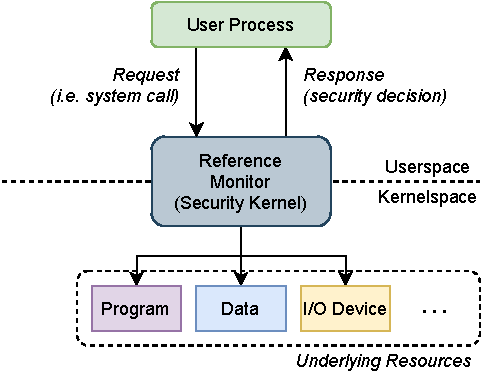
\includegraphics[width=0.6\linewidth]{figs/background/refmon.pdf}
  \caption[The reference monitor concept]{
    The reference monitor concept as outlined in the Anderson Report. Redrawn and adapted
    from Anderson~\cite{anderson1972_report}. User processes make requests (e.g.\ via
    system calls to the operating system). The \gls{os} kernel invokes the reference
    monitor, which is implemented in software as a security kernel. The reference monitor
    queries its security policy taking the subject, object, and other parameters as input.
    As output, it returns a security decision (i.e.\ whether the requested access should be
    \textit{allowed} or \textit{denied}).
  }\label{fig:refmon}
\end{figure}

While the majority of modern operating systems do not include a security kernel as
described by Anderson, the reference monitor architecture has informed the design of
modern access control mechanisms and models the reference validation process that occurs
when the kernel is servicing userspace requests (i.e.\ system
calls)~\cite{van_oorschot2020_tools_jewels}. In order for such a design to be considered
valid, Anderson enumerates three key properties: (i) Tamper Resistance; (ii) Complete
Mediation; and (iii) Verifiability. These properties facilitate reasoning about the
security of modern access control mechanisms, even if they do not strictly adhere to the
reference monitor model.

\paragraph*{Tamper Resistance}

In order for the reference monitor to be considered \textit{tamper resistant}, an unauthorized
party must not be able to alter the reference monitor's code or modify any data
(e.g.\ memory, persistent storage) that the reference monitor relies on to enforce correct
reference validation~\cite{anderson1972_report}. This property follows from the fact that
unauthorized tampering with the reference monitor totally invalidates any security
guarantees.

\paragraph*{Complete Mediation}

The property of \textit{complete mediation} means that the reference monitor should be
invoked on all security sensitive events. It should be impossible for an attacker to
bypass the reference monitor in any way. Any software that is not subject to reference
validation should be considered a part of the reference
monitor~\cite{anderson1972_report}.

\paragraph*{Verifiability}

\textit{Verifiability} refers to the ability to reason about or prove the correctness of
the reference monitor (i.e. that the first two properties hold). Formal verification methods
are the best way of achieving verifiability, although this may not necessarily be practical
for highly complex systems. For this reason, it is recommended to design the reference monitor
in such a way that verifiability is maximized~\cite{anderson1972_report}.

\subsection{Virtual Memory and Memory Protection}\label{ss:virtual-memory}

Virtual memory~\cite{denning1970_virtual} is a mechanism for mapping \textit{virtual}
memory addresses to \textit{physical} machine addresses. First introduced in the 1950s,
the original goal of virtual memory was to make it easier for programmers to manipulate
memory without worrying about the underlying details of storage
configuration~\cite{denning1970_virtual}. With the advent of multi-processing systems,
virtual memory took on a new role\,---\,separation of memory resources between distinct
user processes. This separation is a fundamental notion for secure multi-processing; two
user processes should not be able to interfere with each other's memory, and a user
process should not be able to interfere with the \gls{os} kernel, resident in ring
0 memory.

By partitioning memory into virtual address spaces, virtual memory forms the most
fundamental isolation barrier between user processes. To accomplish this goal, a hardware
mechanism, the \gls{mmu}, translates virtual addresses to physical addresses using
a \textit{page table} maintained by the operating system in main memory. To accelerate the
translation of memory addresses, processors cache this mapping in a specialized
cache area called the \gls{tlb}.  In Unix, each user process gets its own virtual address
space by default, maintained in a per-process page table. Where necessary, this isolation
may be voluntarily broken using memory sharing mechanisms provided by the \gls{os} kernel
(e.g.\ multi-threading or shared memory mappings). The kernel also gets its own address
space which maps the entirety of physical memory.

While virtual memory can help isolate user processes from each other and user process from
the kernel, additional protection mechanisms are required to strengthen this isolation. To
this end, the \gls{cpu} \gls{isa} generally defines memory protection bits that can be applied
to physical pages and enforced in the \gls{mmu}. For instance, individual pages can be
marked as readable, writable, and/or executable depending on how the memory is to be used.
How these protections are used is generally up to the operating system; for instance,
modern operating systems often enforce a policy where pages marked writable are not
allowed to be marked executable and vice versa (this is often referred to as W$\oplus$X).
This helps to prevent basic buffer overflow attacks. Another important
protection mechanism employed by the operating system is \gls{aslr}, which slightly
randomizes virtual address space mappings, making them unpredictable and thus more difficult for
attackers to exploit consistently. A similar mechanism, \gls{kaslr}, protects the kernel.
The \texttt{grsecruity} patch suite~\cite{grsecruity} offers additional memory protection for the
Linux kernel, hardening the boundary between userspace and kernelspace and applying
additional mitigations to prevent return oriented programming attacks.

Additional protections are afforded by \textit{memory protection rings}, a concept first
introduced by Multics~\cite{vyssotsky1965_multics, corbato1965_multics} in the mid-1960s.
In the original design, 64 protection rings were defined in hardware, numbered from 0--63.
A task running in a higher-numbered protection ring would be unable to access any memory
marked with a lower-numbered protection ring, effectively isolating sensitive code and
data from unprivileged tasks. Modern \glspl{cpu} carry forward this notion of protection
rings, although a typical modern processor only defines far fewer protection rings in
practice. For instance, x86 only implements four protection rings in total. Modern
\gls{os}s, including Linux, generally only use \textit{two} of these rings, ring 0 and
ring 3 (on x86 processors) for kernelspace and userspace respectively.  \Cref{fig:rings}
depicts this design. Lee \etal~\cite{lee2018_lotr} have proposed using the remaining two
rings for finer-grained isolation on x86.

\begin{figure}[htbp]
  \centering
  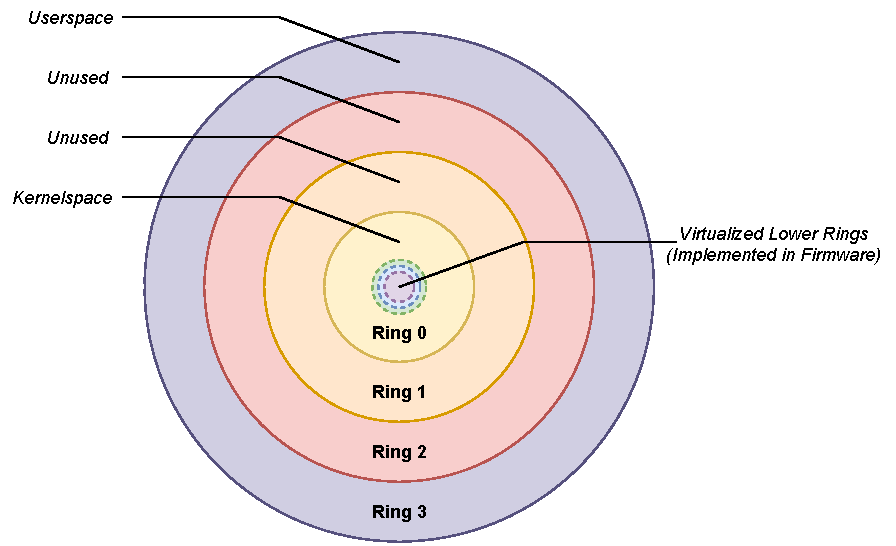
\includegraphics[width=0.8\linewidth]{figs/background/rings.pdf}
  \caption[Protection rings on modern \glsentryshortpl{cpu}]{
    A visualization of protection rings on x86 \glsentryshortpl{cpu}. Ring 3 contains
    \textit{userspace}, the address space of ordinary applications that run in user mode.
    Ring 0 contains \textit{kernselspace}, the kernel's address space. Code running in
    ring 0 is said to run in \textit{supervisor mode}. Rings 1--2 are generally unused by
    \glsentryfull{cots} operating systems. \glsentryshortpl{cpu} often implement \enquote{lower}
    rings (-1, -2, etc.) by virtualizing ring 0 in firmware. These are typically reserved
    for the hypervisor and other hardware-backed features like Intel's System Management
    Mode~\cite{tereshkin2009_introducing}.
  }\label{fig:rings}
\end{figure}

\subsection{Discretionary Access Control}\label{ss:dac}

\textit{\glsentryfull{dac}} comprises the most basic form of access
control in many operating systems, including Linux, other Unix-like operating systems, and
Microsoft Windows. First formalized in the 1983 US Department of Defense
standard~\cite{orange_book}, a discretionary access control mechanism partitions and
labels system objects (i.e.\ resources such as files) by the subjects (i.e.\ actors such as
users and user processes) that \textit{own} them. The corresponding resource owner then
has full authority to decide which subjects have access to its owned objects. This notion
of ultimate authority over a subject's owned objects constitutes the primary difference
between discretionary access control and mandatory access control, which is covered in
\Cref{ss:mac}.

Classically, Unix-like systems have implemented discretionary access control in the form
of \textit{permission bits} and \textit{access control lists}. Each process on the system
runs under a specific user and group ID, which uniquely identify the user and group of the
process respectively, where each group is a collection of one or more users. Permission
bits and access control lists denote access permissions according to the user ID and group
ID of the process requesting the resource. These permissions can in turn be overridden by
the \textit{superuser} or \textit{root}~\cite{van_oorschot2020_tools_jewels,
jaeger2008_os_security}.

\subsubsection*{Permission Bits}

Permission bits in Unix are special metadata associated with a file that determine
coarse-grained access to the file according to a subject's \gls{uid} and \gls{gid}.
Permission bits are divided into three sections: \textit{User}, \textit{Group}, and
\textit{Other}. The \textit{User} bits apply to subjects whose \gls{uid} matches the
resource owner's \gls{uid}, while the \textit{Group} bits consider the \gls{gid} instead.
In all other cases (i.e.\ when neither the \gls{uid} nor the \gls{gid} matches), the
\textit{Other} bits determine the allowed access. To determine which access should be
allowed, permission bits encode a coarse-grained \textit{access vector}, specifying read,
write, and execute access on a file or directory (in the case of a directory, execute
access implies the ability to \texttt{chdir(2)} into that directory).

While convenient, permission bits are generally insufficient to provide legitimate
security guarantees to modern systems~\cite{van_oorschot2020_tools_jewels,
jaeger2008_os_security}. In particular, permission bits encode coarse-grained permissions
and apply these permissions in a coarse-grained, all-or-nothing, manner. For instance,
consider the use case of granting read-only access to another user. Specifying such access
as part of the \textit{Other} bitmask implies granting access to any user on the system.
Specifying access to a particular \textit{Group} is slightly better, but the resource
owner has no direct control over which other users belong to this group, now or in the
future. Thus, we cannot say with certainty that we may specify such access without
violating our security assumptions.

\subsubsection*{Access Control Lists}

\Glspl{acl} offer a slightly more granular alternative to permission bits,
at the expense of increased complexity~\cite{jaeger2008_os_security,
van_oorschot2020_tools_jewels}. Unlike permission bits, which rely on three coarse-grained
subject categories (\textit{User}, \textit{Group}, and \textit{Other}), an access control
list defines a set of subjects and their corresponding permissions for every object. It
may be helpful to think of this as breaking up the \textit{Other} category into distinct
subjects rather than granting or revoking blanket access to all other users on the system.

Capability lists, complementary to access control lists, define a set of objects and
allowed access patterns for every subject. A capability list for a given subject can be
derived by taking the set of all access control lists for every object and vice
versa~\cite{van_oorschot2020_tools_jewels}. Together, the set of all access control lists
(or capability lists) forms an \textit{access matrix}, describing the \gls{dac} policy over
the entire system. \Cref{fig:acl} depicts this relationship.

\begin{figure}[htbp]
  \centering
  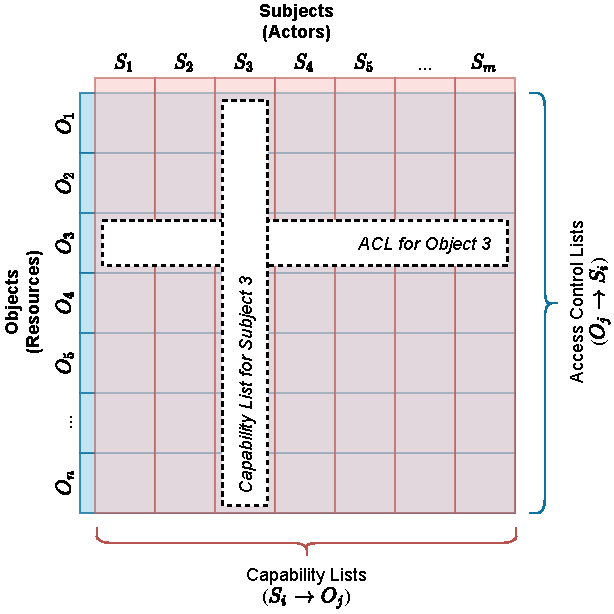
\includegraphics[width=0.8\linewidth]{figs/background/acl.pdf}
  \caption[The access matrix]{
    The access matrix and the relationship between \glspl{acl} and capability
    lists~\cite{anderson1972_report, van_oorschot2020_tools_jewels,
    jaeger2008_os_security}. \glspl{acl} define the set of subjects that have specific
    access rights on a particular object. Capability lists conversely define the access
    rights that a specific subject has on a set of objects. Note that an \gls{acl} may be
    derived by taking the set of all capability lists and vice versa. Taken together,
    these form the access matrix.
  }\label{fig:acl}
\end{figure}

\subsubsection*{The Superuser and Setuid}

To facilitate system administration, many \gls{dac} schemes incorporate the notion of
a \textit{superuser} or \textit{administrator role} into their model. In Unix and
Unix-like operating systems, the superuser or \textit{root} user is denoted by the
\gls{uid} of zero. Any process running with the \gls{euid} of zero is said to be
\textit{root-privileged}. These root-privileged processes can then override the system's
\gls{dac} policy, bypassing permission bits and access control entries on system objects.

In many cases, a program requires additional privileges in order to function. For
instance, a \texttt{login} program would require the ability to read security-sensitive
password entries in \texttt{/etc/shadow}. To achieve such functionality, Unix provides
special \texttt{setuid} and \texttt{setgid} permission bits that implicitly set the
effective user and group IDs of a process to those of the file owner.
A sufficiently-privileged process may also change its own \gls{euid} or \gls{egid} at
runtime using the \texttt{setuid(2)} and \texttt{setgid(2)} family of system calls. The
example login program, for instance, could use these system calls to drop its privileges
to those of the user being logged in. While necessary under the Unix \gls{dac} model,
setuid and setgid binaries have long been the target of exploitation, particularly for
privilege escalation attacks~\cite{dittmer2014_setuid, van_oorschot2020_tools_jewels,
jaeger2008_os_security}.

\subsubsection*{User and Group Assignment}

To alleviate concerns with discretionary access control, systems often take the approach
of assigning a unique user and/or group to a specific application. Such applications are
typically security sensitive, such as a privileged daemon or network-facing service. This
technique achieves a dual purpose: firstly, the application can lock down any resources it
owns, simply by restricting any access to its own \gls{uid}; secondly, the resulting
process no longer needs to run under the same \gls{uid} as its parent. This effectively
limits the amount of outside resources that the application can access (so long as
permission bits are correctly configured).

The Android operating system takes this model a step further, assigning a unique \gls{uid}
and \gls{gid} to every application on the system, with optional \gls{uid} sharing between
applications that come from the same vendor. Under this model, no process' \gls{uid} ever
corresponds to a human user. While this arguably improves security, Barrera
\etal~\cite{barrera2012_android} found weaknesses in Android's \gls{uid} sharing model
that can reduce its security to the trustworthiness of an app's signing key.

\subsubsection*{DAC Security Assumptions and Attacks}

Although discretionary access control provides a convenient and intuitive user-centric
model for object ownership and permissions, it makes some dangerous assumptions about
security that can totally invalidate the model in
practice~\cite{shu2016_security_isolation_study}. In particular, \gls{dac} assumes that all
processes are benign and contain no exploitable vulnerabilities. The mere existence of
malware and exploitable vulnerabilities (e.g.\ memory safety vulnerabilities) immediately
invalidates this assumption. For instance, consider an honest but vulnerable piece of
software running under a given \gls{uid} $X$. An attacker exploiting a vulnerability in
this application could perform arbitrary operations on any files owned by $X$. Similarly,
a Trojan horse\footnote{A Trojan horse is a piece of ostensibly benign software that
is designed to perform some malicious action or actions in addition to its ordinary
functionality~\cite{van_oorschot2020_tools_jewels}.}~\cite{shu2016_security_isolation_study,
van_oorschot2020_tools_jewels} can perform arbitrary malicious operations on $X$'s files
without needing to exploit any vulnerability. The fundamental issue with Unix \gls{dac} is
that these files need not necessarily have \textit{anything} to do with the program in
question.

Another fundamental issue with Unix \gls{dac} lies in the ultimate authority of the root
user. Any process running with \gls{euid}=0 is immediately part of the system's
\gls{tcb}\footnote{The \textit{trusted computing base} is the set of all hardware
and software that must be trusted in order for the system to be considered trusted.
Typically, this includes system hardware, the operating system itself, and a small subset
of userspace programs~\cite{jaeger2008_os_security}.}. The same applies to any executable
marked as setuid root. Processes that run with root privileges are prime targets for
attacker exploit, since a successful attack can effectively compromise the entire system.
For instance, confused deputy attacks~\cite{hardy1988_confused_deputy,
shu2016_security_isolation_study} can exploit privileged processes by tricking them into
performing some undesired action. The coarse granularity of Unix \gls{dac} renders it
particularly vulnerable against such attacks.

\subsubsection*{Proposals for Alternative Schemes}

Both industry and academia have long recognized that weaknesses in the Unix discretionary
access control model must be addressed. Many have turned to mandatory access
control~\cite{spencer1999_flask, smalley2001_selinux, wright2002_lsm, cowan2000_apparmor,
schaufler_smack, schreuders2012_towards, hu2013_fsf, harada2004_tomoyo, salaun_landlockio,
singh2019_krsi} (c.f.\ \Cref{ss:mac}) to solve the fundamental issues in \gls{dac}, while
others have proposed improvements or alternative schemes for implementing discretionary
access control~\cite{mao2009_trojan_resistant_dac, solworth2004_layered_dac,
dranger2006_dac_complexity, dittmer2014_setuid, tsafrir2008_setuid, chen2002_setuid}. This
subsection focuses specifically on the latter.

Mao \etal~\cite{mao2009_trojan_resistant_dac} proposed IFEDAC (Information Flow Enhanced
\glsentryshort{dac}) as an alternative \gls{dac} model that is resistant to Trojan horse
attacks.  The insight behind their work was that \gls{dac}'s primary weaknesses lie in the
inability to distinguish requests involving multiple actors. Their mechanism proposes to
track information flows between subjects and use these flows to infer a list of subjects
that have influenced a request.

Under the traditional Unix \gls{dac} model, only the \gls{uid} and \gls{gid} of the
process are considered when making access control decisions; under IFEDAC, the \gls{uid}
and \gls{gid} of the owner of the underlying executable would also be considered, along
with any other parties that may have influenced the state of the running process. This
approach is similar in spirit to taint tracking mechanisms~\cite{livshits2012_dynamic}
(c.f.\ \Cref{ss:taint-tracking}). To enable programs to function correctly, IFEDAC enables
the user to define \textit{exception policy} that specifies exceptions to IFEDAC
enforcement. Mao \etal~recommend that application authors and OS vendors should be
responsible for distributing such policies~\cite{mao2009_trojan_resistant_dac}.

Dranger, Solworth, and Sloan~\cite{solworth2004_layered_dac, dranger2006_dac_complexity}
presented a three-layered model of \gls{dac} mechanisms. The \textit{base layer} defines
the general access control model, while the \textit{parameterization layer} parameterizes
it according to deployment needs.  Finally, the \textit{local initialization layer}
comprises the set of subjects and objects along with their associated protections. The
authors showed that their model was generalizable and that it could be used to implement
any \gls{dac} mechanism.

Dittmer and Tripunitara~\cite{dittmer2014_setuid} examined the implementation and common
usage patterns of the POSIX setuid and setgid \gls{api} across multiple Unix-like operating
systems. They identified weaknesses in systems that do not implement the latest POSIX
standard revisions and suggested that mismatched semantics between various implementors
can be a source of developer error. Finally, they presented an alternative \gls{api} that
partitions \gls{uid} changes into permanent and temporary categories. Tsafrir
\etal~\cite{tsafrir2008_setuid} and Chen \etal~\cite{chen2002_setuid} identified the same
fundamental issues and proposed the adoption of similar mechanisms.






\section{Extensions to the Unix Security Model}\label{s:security-extensions}

Having examined the classical components of an operating system security framework, we now
turn our attention to recent extensions on top of the Unix security model, with
a particular emphasis on Linux and other free and open source Unix-like operating systems.
This section presents a selection of key developments on top of the original Unix security
model which have developed over time, with a particular emphasis on process-level
confinement.





\subsection{POSIX Capabilities}

POSIX capabilities~\cite{posix_capabilities, corbet2006_capabities_a,
corbet2006_capabities_b} are highly related to Unix \gls{dac} in the sense that they were
originally designed to break up the multitude of privileges associated with the
\textit{root} user into more manageable pieces. In this sense, POSIX capabilities (when
properly used) are more conducive to the principle of least-privilege. A process need not
necessarily possess full root-level access to the system when only a small subset of those
privileges are actually required.

Originally specified in the (now withdrawn) 1003.1e POSIX standard, POSIX capabilities
were only ever (partially) implemented on Linux~\cite{anderson2017_comparison}. Other
Unix-like operating systems prefer alternative methods of restricting privileges, many of
which are discussed in \Cref{ss:syscall-filtering}. POSIX capabilities specify three
\textit{capability sets} for a given process: the \textbf{bounding set}, the
\textbf{inheritable set}, and the \textbf{effective set}. The bounding set determines the
set of all capabilities that a process is ever allowed to possess. The inheritable set
determines the set of all capabilities that can be inherited across \texttt{execve} calls.
Finally, the effective set determines the set of capabilities that a process can use
(i.e.\ which capabilities a process currently possesses).

Linux exposes POSIX capabilities through extended filesystem attributes, much the same way
that \glspl{acl} are implemented~\cite{corbet2006_capabities_b}. These file-based
capabilities function in a similar manner to the setuid bit, implicitly setting the
bounding, inheritable, and effective capability sets on execution. In addition so
supporting capabilities as extended filesystem attributes, the kernel also supports
dropping specific capabilities from each of the three sets through the \texttt{ptrctl(2)}
system call. This enables a higher-privileged process (e.g.\ running as root) to drop
elevated privileges while retaining those it needs to function. As of Linux 5.12, the
kernel supports 41 capabilities in total, including the all-encompassing
\texttt{CAP\_SYS\_ADMIN}~\cite{linux_capability_h}.

It is worth mentioning that the term \enquote{POSIX capabilities} does \textit{not}
describe capabilities as they are broadly defined by operating system security
researchers~\cite{anderson2017_comparison}. In particular, Dennis and Van
Horn~\cite{dennis1966_semantics} first defined the notion of capabilities as a means of
restricting access to \textit{pointers}, guarding references to system objects. Unlike the
capabilities defined by Dennis and Van Horn, POSIX capabilities are not associated with
any given system object. Dennis and Van Horn's capabilities more closely resemble that of
the access matrix introduced by Anderson~\cite{anderson1972_report} and similar mechanisms
have been implemented in other systems such as FreeBSD's
Capsicum~\cite{watson2010_capsicum} and the CHERI architecture~\cite{watson2015_cheri,
davis2019_cheriabi}. These are discussed in more detail in \Cref{ss:syscall-filtering}.

\subsection{Mandatory Access Control}\label{ss:mac}

In contrast with \gls{dac}, \textit{\gls{mac}} does not delegate permission assignment to
the resource owner~\cite{spencer1999_flask, van_oorschot2020_tools_jewels,
jaeger2008_os_security}. In the context of Unix, this means that \gls{mac} both overrides
traditional discretionary access controls \textit{and} applies access controls to all
users on the system, including root. Historical implementations of \gls{mac} have focused
primarily on \gls{mls}, an access control scheme that revolves around the \textit{secrecy}
of objects and \textit{access level} of subjects~\cite{bell2005_blp}. In a nutshell,
\gls{mls} prevents a subject from reading data with a higher secrecy level or writing data
with a lower secrecy level, preventing breaches in confidentiality and
integrity~\cite{jaeger2008_os_security}.

\subsubsection*{Historical Approaches}

Multics~\cite{vyssotsky1965_multics, corbato1965_multics} was the first operating system
to pioneer the use of an \gls{mls} access control scheme. Memory in Multics was
virtualized into \textit{segments}, each with a \textit{segment descriptor} that outlined
protections that should be applied to that memory. To define an \gls{mls} policy, these
protections included a secrecy level, enforced according to the subjects secrecy level.
These \gls{mls}-style protections were complementary to discretionary \gls{acl}s defined
for every segment along with memory protection rings (the first of their kind), enforced
in hardware~\cite{jaeger2008_os_security}.

While \gls{mls} is primarily applicable to military contexts, \gls{mac} has since evolved
into mainstream use through the advent of alternative implementations. The Flask
microkernel~\cite{spencer1999_flask} introduced a practical architecture for \gls{mac}
policy enforcement that was both scalable and effective. The non-discretionary components
of the Flask security model were hugely influential in the design and implementation of
subsequent \gls{mac} enforcement mechanisms, most notably
SELinux~\cite{smalley2001_selinux, loscocco2001_selinux}.

The basic notion behind flask is straightforward; the security architecture is divided
into a security server, responsible for storing security policy, and a object manager that
serves requests to userspace applications. When an application requests a resource, the
object manager queries security policy from the security server and decides whether or not
to serve the request based on the resulting enforcement decision. By designing Flask to be
modular in this way, Spencer \etal~achieved a separation of concerns between policy
enforcement and policy decision-making, vital for scalability~\cite{spencer1999_flask,
smalley2001_selinux, loscocco2001_selinux}.

\subsubsection*{Linux Security Modules, SELinux, and AppArmor}

The NSA first introduced SELinux (Security Enhanced Linux)~\cite{smalley2001_selinux,
loscocco2001_selinux} as a Linux kernel patch, with the goal of providing an
implementation of the Flask security architecture~\cite{spencer1999_flask} for the Linux
kernel. Reluctant to restrict users to just one security architecture, the kernel
community eventually agreed that a generic security framework would provide more value
than a single implementation, allowing for multiple upstream security implementations that
could be selected based on the downstream use case. This effort culminated in the
introduction of the \textit{Linux Security Modules} (\gls{lsm})~\cite{wright2002_lsm} framework.

The \gls{lsm} framework consists of a set of security hooks, placed in strategic locations
throughout the kernel~\cite{wright2002_lsm}. Hooks can roughly be divided into
\textit{enforcement} hooks and \textit{bookkeeping} hooks. Enforcement hooks serve as
checkpoints for security enforcement over specific access categories, while bookkeeping
hooks enable a security module to maintain stateful information about subjects and objects
on the system.  \gls{lsm} hooks are not considered to be static, and often change between
kernel versions as new hooks are implemented and both new and existing hooks placed into
various kernel functions~\cite{zhang2021_lsm_file_overhead}. The eventual goal of the
\gls{lsm} framework is to provide complete mediation over kernel security events, however
this is an evolving process and no formal verification exists to prove the security of
\gls{lsm} hooks~\cite{ganapathy2005_lsm}. \Cref{fig:lsm} depicts the basic \gls{lsm} architecture.

\begin{figure}[htbp]
  \centering
  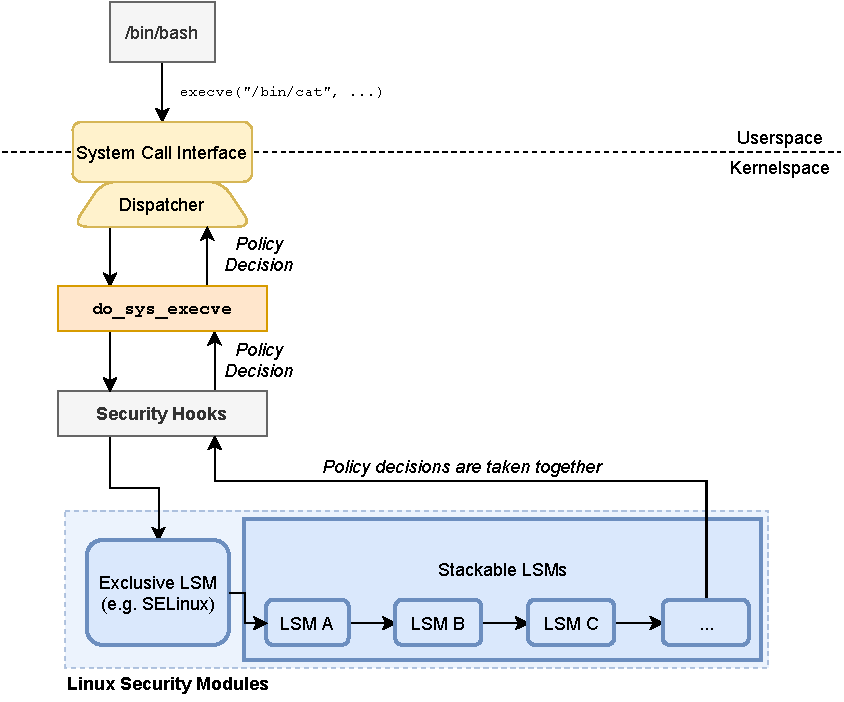
\includegraphics[width=0.8\linewidth]{figs/background/lsm.pdf}
  \caption[The \glsentryshort{lsm} architecture]{
    The \gls{lsm} architecture. A single \textit{exclusive} \gls{lsm} may be loaded at a time,
    and complemented by zero or more \textit{stackable} \gls{lsm}s. When userspace
    requests a privileged operation (e.g.\ through a system call), this operation causes one
    or more security hooks to be invoked. These hooks in turn call into the respective
    hook implementations provided by each loaded \gls{lsm}. Each hook returns a policy
    decision, and these decisions are then taken together to arrive at a final decision.
  }\label{fig:lsm}
\end{figure}

After the introduction of the \gls{lsm} framework, SELinux was refactored into a Linux
security module~\cite{smalley2001_selinux} and subsequently merged into the mainline
kernel. SELinux supports three major types of mandatory access control: (i) role-based
access controls; (ii) type enforcement; and (iii) an optional \gls{mls} policy.
Fundamentally, SELinux policies are based on a notion of subject and object labelling.
A security policy assigns a specific label to subjects and objects, and then specifies
access patterns between these labels.

In an effort to simplify the SELinux policy language, a \textit{reference policy} was
introduced by PeBenito in 2006~\cite{pebenito2006_refpol}, providing a framework for
creating and managing reusable policy templates which can be integrated into new and
existing security policies. SELinux reference policies can be augmented with boolean
options, called \textit{tunables} that provide coarse-grained control over policy
behaviour to system administrators. Sniffen~\cite{sniffen06_guided} implemented a guided
policy generation system that walks application authors through the process of writing
SELinux policy. This framework was further augmented by
MacMillan~\cite{macmillan07_madison}, culminating in the eventual introduction of the
\texttt{audit2allow}~\cite{audit2allow} command line utility for automated policy
generation. Despite these usability improvements, the SELinux policy language is generally
considered to be quite arcane~\cite{schreuders2012_towards}, rendering it difficult for
non-expert users to write and audit security policy.

Since the introduction of SELinux, several alternative \gls{lsm}s have been proposed, many
of which have subsequently been merged into the mainline Linux kernel. AppArmor
(originally called SubDomain)~\cite{cowan2000_apparmor} takes an alternative approach to
SELinux, enforcing security policy based on \textit{pathnames} rather than security
labels.  AppArmor policies, called \textit{profiles}, are assigned on a per-executable
basis. Rather than being labelled, AppArmor policies identify system objects directly
(e.g.\ through pathnames, \gls{ipc} categories, or network \gls{ip} addresses). Each system
object is associated with a particular access pattern, which determines the privileges for
a given AppArmor profile. Similar to SELinux, AppArmor offers a suite of userspace tooling
for automated and semi-automated policy generation based on enforcement
logs~\cite{aa_easyprof, aa_genprof, aa_logprof}.

\subsubsection*{Alternative Linux Security Modules}

Recognizing usability issues in the complexity of SELinux and AppArmor policies,
Schaufler~\cite{schaufler_smack} introduced SMACK (Simplified Mandatory Access Control
Kernel) to offer a simplified label-based enforcement scheme that focuses on expressing
a minimal set of permissions. Like SELinux, SMACK relies on labelling filesystem objects
using extended filesystem attributes. Policies then attach simple access specifiers to
these labels, based on canonical Unix permissions like \texttt{read}, \texttt{write}, and
\texttt{execute}. Some default labels are provided, which grant or revoke blanket
permissions for common tasks such as system daemons or the \texttt{init} process.

Schreuders \etal~\cite{schreuders2012_towards} designed FBAC-LSM (Functionality-Based
Access Control \gls{lsm}) with a similar goal of simplifying policy definition. Unlike
SMACK, which is based on labelling, FBAC-LSM specifies policy in terms of desired
\textit{functionality}. Specifically, FBAC-LSM policies define a set of high-level
functionalities that an application should exhibit. All other functionalities are
prohibited. Schreuders \etal~evaluated FBAC-LSM in terms of its usability and found that
it compares favourably against AppArmor and SELinux~\cite{schreuders2012_towards}.

Hu \etal~\cite{hu2013_fsf} proposed FSF (File System Firewall), which applies
firewall-like semantics to filesystem objects. Their goal was to create a more usable,
file-specific access control mechanism. FSF policies are defined in policy files,
comprised of simple rules that specify a file along with some combination of
\texttt{read}, \texttt{write}, and \texttt{execute} access. \textit{Redirection rules} are
primary differentiating factor between FSF and conventional file-based access controls.
Taking inspiration from similar functionality in network firewalls, a redirection rule can
be used to convert one file access into another, transparently to the target application.
Hu \etal~conducted a user study comparing their prototype to Unix \gls{dac} and SELinux
and found that FSF performed favourably in policy comprehensibility and accuracy.

The TOMOYO~\cite{harada2004_tomoyo} \gls{lsm} takes an alternative approach, emphasizing
policy generation and building generation functionality into the \gls{lsm} directly.
Rather than involving userspace helpers, TOMOYO generates policy by inferring
per-application profiles through the \gls{lsm} hooks they invoke. Programs can
additionally discard their privileges through a TOMOYO-specific system call, similar to
the notion of dropping privileges under the POSIX capabilities model. Like AppArmor,
TOMOYO relies on pathnames to identify resources rather than assigning security labels.
Users have the option to edit generated policies as required, but the intent is to require
as little user involvement as possible~\cite{harada2004_tomoyo}.

The Landlock~\cite{salaun_landlockio, salaun_landlock_patch} \gls{lsm} was recently
introduced into the mainline Linux kernel as a contemporary alternative to
\texttt{seccomp(2)} (covered in \Cref{sss:seccomp}). Landlock was originally intended to
allow unprivileged userspace processes to load highly restricted \gls{ebpf} programs into
the kernel to define security filtering logic~\cite{salaun_landlock_patch}. However, due
to concerns related to the security of unprivileged \gls{ebpf}, this functionality was
later reworked into a set of simple access rules and no longer has any association with
\gls{ebpf}~\cite{salaun_landlockio}. Under Landlock, a process creates a \textit{ruleset}
using the \texttt{landlock\_create\_ruleset(2)} system call, adds rules to that ruleset,
then confines itself by committing to that ruleset. Developers may add this confinement
logic directly into their software or may write specialized userspace wrappers to apply
generic confinement to applications.

Singh~\cite{singh2019_krsi} introduced the KRSI (Kernel Runtime Security Instrumentation)
framework for attaching \gls{ebpf} programs to \gls{lsm} hooks with the goal of defining
dynamic audit and policy enforcement filters. While similar in spirit to the original
Landlock proposal~\cite{salaun_landlock_patch}, KRSI differs fundamentally in that it
remains a \textit{privileged} \gls{lsm}; only root-privileged processes may load
\gls{ebpf} \gls{lsm} programs into the kernel. \bpfcontain{} and \bpfbox{} are both based
on the KRSI framework. \Cref{ss:bpf-programs-bg} examines the KRSI framework in more
detail.





\subsection{System Call Filtering and Capabilities}\label{ss:syscall-filtering}

Since system calls define the canonical interface for communication between userspace
processes and the operating system kernel~\cite{jaeger2008_os_security}, they are
a natural fit for defining the protection interface of a confinement mechanism. In
particular, \textit{system call filtering} is a widely-used technique for application
sandboxing and self-confinement~\cite{anderson2017_comparison}. Indeed, \gls{lsm}s,
covered in the previous section, can be thought of as a form of system call filtering,
although security hooks are placed manually within system call implementations and do not
necessarily conform to the same semantics as the underlying system
calls~\cite{wright2002_lsm}.

Related to this notion of system call filtering are \textit{capabilities}\footnote{Here,
the term \enquote{capabilities} is a disparate term from \enquote{POSIX capabilities,}
covered in \Cref{ss:dac}.}, which guard access to a particular reference, associating
privileges with a handle to a given object on the system. For instance, the
\texttt{open(2)} system call returns a \textit{file descriptor}, which constitutes
a reference to a particular filesystem object. A capability associated with this file
descriptor would then allow specific operations on the file descriptor, applying
a default-deny policy to all other operations.

\subsubsection*{System Call Tracing}
\label{sss:ptrace}

In Unix, ptrace~\cite{ptrace, padala2002_ptrace} (short for process trace) is a mechanism
provided by the kernel that allows one process (the tracer) to attach itself to another
(the tracee), tracing and possibly manipulating nearly any aspect of its execution, system
calls, memory, and registers. Originally designed as a debugging interface~\cite{ptrace,
padala2002_ptrace}, ptrace has also been applied to implement system call
filtering~\cite{goldberg96_janus, wagner1999_janus, jain2000_filtering}. However, ptrace
has fallen out of favour, particularly in production use cases, due to its immensely high
overhead (on the order of several thousand percent~\cite{zinke2009_overhead}) and
propensity to introduce undefined behaviour when tracing even moderately complex
software~\cite{swiecki2017_promises}. Due to its invasive nature, a tracer process must
either be the direct parent of a tracee or must have sufficient privileges to trace the
child process\,---\,on Linux, this translates to either the \texttt{CAP\_SYS\_PTRACE}
capability or the all-encompassing \texttt{CAP\_SYS\_ADMIN}.

Janus~\cite{goldberg96_janus, wagner1999_janus} was an early exploration of how
\texttt{ptrace} could be applied to confine applications by filtering system calls.  The
original Janus prototype was designed for Oracle Solaris using its ptrace interface,
exposed through the \texttt{procfs} virtual filesystem~\cite{goldberg96_janus}.
A subsequent port of Janus was released for Linux~\cite{wagner1999_janus}, although it
required invasive modifications to Linux's ptrace implementation, dubbed ptrace++ by the
authors. Janus worked by attaching to the target process using ptrace, then tracing system
calls made by the target process and categorizing them into groups based on functionality.
A Janus policy could allow or deny specific categories of system call, confining the
application in a coarse-grained manner. The tracer process, called the \textit{supervisor
process}, would then be able to kill the offending process or inject failure into the
offending system call when it detected a policy violation.  Jain and
Sekar~\cite{jain2000_filtering} implemented a similar system call monitor, adding the
ability to modify system call arguments and using a different policy language design.

Provos' Systrace~\cite{provos2003_systrace} uses ptrace to analyze per-process system
calls and generate a system-call-level policy. Unlike Janus~\cite{goldberg96_janus,
wagner1999_janus} and Jain~\etal~\cite{jain2000_filtering}, Systrace supports intrusion
detection, policy generation, and audit logging, providing a mechanism to automatically
analyze process behaviour. Systrace also supports one highly unconventional feature, which
Provos calls \textit{privilege elevation}. The notion behind privilege elevation is to
allow a program to escalate its privileges selectively for specific system call access
patterns, preventing the need for coarse-grained privilege escalation such as setuid root.

Somayaji and Forrest~\cite{somayaji2000_ph} implement an intrusion detection system, pH
(process Homeostasis), based on system call sequences, although it does not rely on ptrace
and analyzes system call sequences instead of individual call patterns. Rather than as
a confinement solution, pH was strictly designed as a behavioural anomaly detection
system, although this approaches confinement as profile accuracy improves.
Findlay~\cite{findlay2020_ebph} (the author of this thesis) later ported pH to use
\gls{ebpf} to analyze system call sequences.

\subsubsection*{OpenBSD Pledge and Unveil}
\label{sss:pledge}

OpenBSD's \texttt{pledge(2)} and \texttt{unveil(2)} system calls form the backbone of its
built-in sandboxing framework. A pledge~\cite{pledge} consists of a list of
\textit{promises}, high-level descriptions of what behaviours a program expects to exhibit
in the future, similar in spirit to Janus' high-level categories~\cite{goldberg96_janus,
wagner1999_janus}. The pledge system call takes two space-separated lists of promises, one
to be applied immediately and another to be applied upon making an \texttt{execve(2)}
call. To prevent privilege escalation, subsequent calls to \texttt{pledge(2)} take the
union of existing promises and new promises, precluding a process from escaping its
initial bounding set~\cite{pledge}.

Promises vary in granularity; the most coarse-grained promise, \texttt{stdio}, allows
a total of 69 distinct system calls, enabling the full suite of C standard library
stdio-family calls. Others, like \texttt{chown}, are more conservative, enabling only one
(albeit in this case very powerful) system call. In total, \texttt{pledge(2)} includes 33
distinct promises, as of OpenBSD 6.9~\cite{pledge}. Due to its coarse granularity and lack
of concern for specific system objects, pledge has been criticized as being
overly-permissive~\cite{anderson2017_comparison}.

Unlike pledge, \texttt{unveil(2)}~\cite{unveil, corbet2018_unveil} operates on specific
filesystem paths, making a promise about the kinds of operations the process will perform
on file descriptors associated with these paths. Specifically, unveil is concerned with
four kinds of permissions: read, write, execute, and create/delete. Unveiling a directory
unveils all files and directories underneath, recursively. Although this approach is
finer-grained than pledge, it is file-specific and offers a trade-off between granularity
and usability. The official manual page for unveil~\cite{unveil} recommends that
developers use it at the granularity of directories, despite the fact that this may result
in overpermission in practice. For instance, consider a hard link to the root of the
filesystem placed by an attacker within some unveiled directory. The unveiling process
would now have full access to the entire filesystem, constituting a sandbox escape.

\subsubsection*{Linux Seccomp and Seccomp-bpf}\label{sss:seccomp}

In Linux, the primary facility for direct system call filtering is
\texttt{seccomp(2)}~\cite{anderson2017_comparison, seccomp, prctl, edge2015_seccomp}.
Unlike OpenBSD's pledge and unveil~\cite{pledge, unveil}, seccomp filters directly over
system calls, without any blanket categorization. Initially, seccomp was highly limited,
restricting a process to only four system calls: \texttt{read(2)} and \texttt{write(2)}
for reading and writing open file descriptors, \texttt{sigreturn(2)} for handling signals,
and \texttt{exit(2)} to enable self-termination. Using any other system call would result
in an immediate SIGKILL delivered from the kernel, forcefully ending the offending
process.

Later, seccomp was extended to enable processes to define custom
allowlists\footnote{Allowlist and denylist are the new politically correct terms (in
addition to being more semantically meaningful) for whitelist and blacklist
respectively.}, denylists, and enforcement actions using classic \gls{bpf}
filters~\cite{edge2015_seccomp}. This new incarnation was dubbed seccomp-bpf.  While
allowing for much finer-grained confinement policy than pledge and unveil, seccomp-bpf has
its own limitations which can result in ineffective (and possibly dangerous) policies. In
seccomp-bpf, filters are defined over system call numbers and (optionally) arguments.
Unless the developer takes great care to correlate system call numbers with the specific
target architecture, the resulting policy may allow and deny incorrect system calls,
resulting in broken policies that break applications in the best case and expose security
vulnerabilities in the worst case.

Another innate problem with seccomp arises due to its fine granularity. Paradoxically,
avoiding system call categorization can expose vulnerabilities, due to system call
equivalence classes. For instance, the \texttt{openat(2)} system call can perform the same
functionality as the \texttt{open(2)} system call, with slightly different \gls{api} semantics.
A seccomp-bpf filter allowing one system call but denying the other is now totally broken
and vulnerable to sandbox escape.  Similarly, argument checking on pathnames or file
descriptors can be vulnerable to \gls{toctou} race conditions in practice, rendering such
policies ineffective~\cite{anderson2017_comparison}.

A final consideration for seccomp-bpf is that the development of seccomp-bpf policies
requires knowledge of the relatively arcane \gls{cbpf} syntax. This problem is somewhat
alleviated by the existence of library wrappers~\cite{libseccomp} around seccomp-bpf
functionality, although the usability of these solutions remains somewhat questionable,
particularly given the many pitfalls of seccomp-bpf policy
authorship~\cite{anderson2017_comparison}.

\subsubsection*{FreeBSD Capsicum and CHERI Capabilities}
\label{sss:capsicum}

Unlike the system call filters presented earlier in this section, FreeBSD's
\texttt{capsicum(2)} \cite{watson2010_capsicum, anderson2017_comparison} is a true
implementation of capabilities as they were originally described by Dennis and Van
Horn~\cite{dennis1966_semantics}. Specifically, capsicum capabilities are an extension on
top of Unix file descriptors, the canonical reference to files and file-like objects such
as network sockets and character devices. Capsicum adds an unforgeable access token to
each file descriptor, granting the corresponding process specific access rights over that
file descriptor. Whereas alternatives like seccomp-bpf~\cite{seccomp} and
pledge~\cite{pledge} restrict access at the system-call-level, Capsicum restricts access
at the resource-level and enforces this access within the system call layer.

To confine processes, Capsicum exposes a special \texttt{cap\_enter(2)} system call which
causes a process to enter \textit{capability mode}. A process in capability mode no longer
has access to global namespaces (e.g.\ the \gls{pid} namespace) and may only make a subset of
system calls which do not directly access these global namespaces. Other system calls are
constrained so that they may only operate under the context of an open capability
descriptor (a file descriptor which has been extended with capability
information)~\cite{watson2010_capsicum}. The end-result is an expressive and fine-grained
self-confinement framework for FreeBSD applications, which comes at a small usability cost
compared with coarser-grained alternatives like \texttt{pledge(2)}~\cite{pledge}.

In 2015, Watson \etal~designed CHERI~\cite{watson2015_cheri} as an extension to the MIPS
\gls{isa} enabling the capability-based protection of memory pages. Under CHERI, the
operating system kernel and userspace runtime extend the traditional memory model with
capabilities using the CHERI \gls{isa}. This enables generic capability-based protection at
the level of memory pages. While powerful, this extension requires dedicated hardware
support. Watson \etal~implemented their prototype on an \gls{fpga}~\cite{watson2015_cheri}
and later extended the FreeBSD \gls{abi} to work with CHERI capabilities~\cite{davis2019_cheriabi}.



\subsection{Taint Tracking}\label{ss:taint-tracking}

\textit{Taint tracking}~\cite{livshits2012_dynamic} describes the notion of tracking
changes to memory containing application data as it is mutated, copied, and moved by the
underlying application. Such data is considered \textit{tainted} when it is modified by
some external source in such a way as the data can no longer be trusted.  For instance,
a buffer might be populated by an external network connection or local user input. The
security benefits of such a mechanism are obvious. An active attack requires some user
input into a program in order to exploit a vulnerability; by tracking untrusted user input
and treating it as untrusted, developers can avoid attacker exploitation of sensitive code
paths. Beginning with Perl's \textit{taint mode}~\cite{hurst2004_perl}, taint tracking has
enjoyed a rich body of literature~\cite{livshits2012_dynamic, conti2010_taint,
bello2012_taint, ermolinskiy2010_towards, zavou2011_taint, yin2007_panorama,
zhu2011_taint_eraser, cheng2006_taint, clause2007_taint, chin2009_efficient} since its
inception.

In Perl's taint mode~\cite{hurst2004_perl}, a special command line flag triggers the
interpreter to flag untrusted user input and prevent it from being passed as input to
functions explicitly marked as \textit{unsafe}. To circumvent this restriction,
a developer could perform a pre-determined set of sanity checks on the data to
\textit{untaint} it. Rather than acting as an outright security mechanism, the goal was to
encourage developers to take care in processing untrusted data. Incorrect or insufficient
sanity checks on the data or running the Perl interpreter without the taint flag would
result in no additional security benefits whatsoever. After Perl, similar taint tracking
mechanisms have been added to other interpreters and language runtimes, including Ruby,
PHP, and Python~\cite{conti2010_taint}.

Conti, Bello, and Russo~\cite{conti2010_taint, bello2012_taint} implemented more advanced
taint tracking functionality for the Python programming language as a library that
developers could use directly. Their argument was that implementing such a taint mechanism
at the language-level rather than at the interpreter-level could enrich the traditional
taint-tracking approach with use-case-specific metadata and facilitate extensions to
support complex data types.

With the goal of creating a generic and reusable taint tracking mechanism, several
researchers have proposed application-transparent taint tracking. Many have turned to
virtualization or emulation runtimes~\cite{ermolinskiy2010_towards, zavou2011_taint,
yin2007_panorama} such as QEMU, KVM, or Xen, using built-in introspection features to
track the propagation of data within (and even between) running processes. Others have
proposed the adoption of static analysis or library
instrumentation~\cite{zhu2011_taint_eraser, cheng2006_taint, clause2007_taint} techniques
to reduce overhead and eliminate the need to run applications under expensive
virtualization monitors. Others have built taint tracking logic into existing language
runtimes, such as the Java Virtual Machine~\cite{chin2009_efficient}.



\section{Process-Level Virtualization}\label{s:virtualization}

We now step away from \textit{confinement} to focus on process-level
\textit{virtualization} primitives employed in Unix-like operating systems. Whereas
confinement primitives have the goal of restricting a process' behaviour, virtualization
primitives instead limit the process' ability to see the world around it. This property
should not be confused with \textit{isolation}. True isolation requires a mixture of both
virtualization and confinement mechanisms to restrict access to system resources and
prevent unwanted behaviour.

\subsubsection*{Chroots and Chroot Jails}

To virtualize the filesystem, Unix has classically supported the \texttt{chroot(2)} system
call~\cite{mcfearin2011_chroot_jails}, used to change the filesystem root (\enquote{\texttt{/}})
to some directory, specified as an argument. From the process' point of view, this
directory becomes its new filesystem root. However, chroot suffers from several issues
that render it totally ineffective as a security mechanism. Chroot escapes, path
traversals, spurious access to special filesystems and devices, and superuser privileges
all totally invalidate chroot as an isolation mechanism~\cite{mcfearin2011_chroot_jails}.

For instance, consider a call to \texttt{chroot("/my/new/root")}. Without a follow-up call
to \texttt{chdir(2)} to change the process' current working directory, a simple call to
\texttt{chdir("..")} is enough to escape the chroot jail. Even with the aforementioned
precautions, a process that has or is able to obtain superuser privileges can simply
create a new directory, re-invoke chroot, and perform the same escape as
before~\cite{mcfearin2011_chroot_jails}. Without the proper confinement mechanisms and
necessary precautions to prevent such escapes, chroot cannot be considered an effective
isolation technique. In fact, chroot escapes have been a source of many vulnerabilities
with container management engines like Docker in the past~\cite{combe2016_to_docker}.
McFearin~\cite{mcfearin2011_chroot_jails} proposed updates to the POSIX standard that fix
many of chroot's security flaws, but these have not been adopted.

\subsubsection*{FreeBSD Jails and Solaris Zones}

Kamp \etal~\cite{kamp2000_jails} presented FreeBSD's \texttt{jail(2)} as a more secure
alternative to \texttt{chroot(2)} jails. In particular, the jail system call is a heavily
extended wrapper around FreeBSD's chroot implementation. A call to jail begins by
allocating and populating a \texttt{prison} data structure that maintains metadata related
to the jailed process group, and finishes by simply invoking the standard chroot
implementation. Unlike chroot, Jails take care to avoid the standard pitfalls that may
result in a chroot escape and heavily limit the privileges of the root user within the
jail. In this respect, the jail system call can be seen as a hybrid between
a virtualization and confinement mechanism, approaching a full solution.

Jails take the approach of defining a clear security boundary around a collection of
processes, filesystem resources, and network resources~\cite{kamp2000_jails}. A process
existing within this boundary (i.e.\ a member of the jail) enjoys the standard set of Unix
permissions on resources within the jail. Access to resources outside of the jail is
forbidden, including access by the root user. Visibility is similarly restricted by
remapping namespaces in such a way as outside resources are effectively invisible.
Defining a clear protection boundary enables the jail to enforce sensible security policy
without burdening the administrator with the details of writing such
a policy~\cite{kamp2000_jails}.

Solaris Zones~\cite{price2004_zones} later arose as a commercial solution for
process-level virtualization. The goal was to implement namespace remapping and security
isolation for commercial server deployments in (possibly multi-tenant) Solaris
environments. The implementation details of Solaris' Zones are similar to those of
FreeBSD's Jails; a per-task data structure manages the associate between tasks and Zones,
allowing the kernel to perform the necessary remapping and security checks.

\subsubsection*{Linux Namespaces and Cgroups}

Unlike FreeBSD~\cite{kamp2000_jails} and Solaris~\cite{price2004_zones}, Linux takes
a different approach to process-level virtualization. In particular, Linux's
virtualization strategy consists of two separate mechanisms, \textit{namespaces} and
\textit{cgroups} (short for process control groups). These mechanisms, in turn, can be
further subdivided into specific types, targeting different kinds of system resources.
Notably, namespaces and cgroups are \textit{not} confinement mechanisms in and of
themselves. This property is in stark contrast with Jails and Zones, which were designed
to offer strong confinement guarantees over their respective security boundaries.
As the canonical process-level virtualization building blocks in Linux, namespaces and
cgroups form the backbone of Linux containers (c.f.\ \Cref{ss:container-security-bg}).

Linux namespaces~\cite{biederman2006_namespaces, linux_namespaces} limit the visibility of
system resource by providing a virtual remapping of global resource identifiers to
a process or process group. Such identifiers include process IDs, user IDs, filesystem
mounts, \gls{ipc} objects, and network interfaces, among others. Linux supports namespace
creation and entry via the \texttt{clone(2)} and \texttt{unshare(2)} system calls, for
isolating child processes and existing processes respectively. As of version 5.13, the
Linux kernel supports eight distinct namespaces, depicted in \Cref{tab:namespaces}. Other
namespaces have been proposed and/or planned for inclusion, including a security
namespace~\cite{sun2018_security_namespace} for virtualizing \gls{lsm} hooks.

\begin{table}
\begin{tabular}{lp{3in}}
    \toprule
    Namespace & Isolates \\
    \midrule
    \multirow{1}{*}{\glsentryshort{pid}} & \glspl{pid}\\
    \multirow{1}{*}{Mount} & Filesystem mountpoints\\
    \multirow{1}{*}{Net} & Networking stack\\
    \multirow{1}{*}{\glsentryshort{uts}} & Host and domain names\\
    \multirow{1}{*}{\glsentryshort{ipc}} & Inter-process communication objects\\
    \multirow{1}{*}{User} & \glspl{uid} and \glspl{gid}\\
    \multirow{1}{*}{Time} & System time\\
    \multirow{1}{*}{Cgroup} & Cgroup membership\\
    \bottomrule
\end{tabular}
\caption[Linux namespaces]{
  Linux namespaces (as of kernel version 5.13) and what they can be used to isolate~\cite{linux_namespaces}.
}
\label{tab:namespaces}
\end{table}

Complementary to namespaces, cgroups~\cite{cgroups, gao2019_houdini} divide processes into hierarchical
groups, performing resource accounting and restricting access to quantifiable resources
such as memory, \gls{cpu} clock cycles, block I/O, and device drivers. From a security
perspective, such restrictions are useful to prevent resource starvation attacks against
the host. However, Gao \etal~\cite{gao2019_houdini} found that this protection is
incomplete and often misleading, allowing up to 200$\times$ the allotted resource limits
by exploiting out-of-band resource consumption techniques. To interact with the cgroup hierarchy,
Linux exposes a virtual filesystem which encodes cgroup membership in its directory structure.
Cgroup membership visibility can be virtualized using the cgroup namespace~\cite{cgroups}.



\section{Containers and Virtual Machines}\label{s:containers-bg}



Classically, virtualization of a system has been accomplished by means of
a hypervisor~\cite{eder2016_hypervisor_container, sultan2019_container_security}.
Hypervisors implement an interface which overlays the underlying system hardware,
enabling one or more \textit{guest operating systems} to be installed on a single physical
host. These guest systems are then called \textit{virtual machines}. Due to the level of
indirection provided by the hypervisor and the guest operating system kernel, virtual
machines are generally considered to be quite \textit{strongly isolated} from each other,
but this isolation comes at the cost of much higher overhead, both in terms of storage and
performance~\cite{eder2016_hypervisor_container, sultan2019_container_security}.
\Cref{s:cp-rethinking} in \Cref{c:confinement-problem} discusses the differences between
virtual machines and containers in more detail and addresses some common misconceptions
about the levels of isolation they provide.





\textit{Containers} have emerged as a new unit of computation in recent years, providing
a more lightweight alternative to full hypervisor-based
virtualization~\cite{sultan2019_container_security, eder2016_hypervisor_container}.
Unlike virtual machines, containers run directly on the host operating system, rather than
directly atop a hypervisor, and share the host operating system kernel with each other and
with ordinary host processes. In fact, a container is nothing more than a discrete
collection of processes (sometimes only one process) that share some common isolation from
the rest of the system by way of virtualization and confinement primitives. These
primitives typically include namespaces and cgroups, along with optional confinement
mechanisms like seccomp-\gls{bpf} and Linux \gls{mac} policy. Since they directly share
the host \gls{os} kernel and do not require a guest operating system, containers are
significantly more lightweight and more performant than virtual machines, but at the cost of
weaker base isolation. \Cref{fig:virt} depicts the major differences between container and
hypervisor-based architectures.



\begin{figure}[htbp]
  \centering
  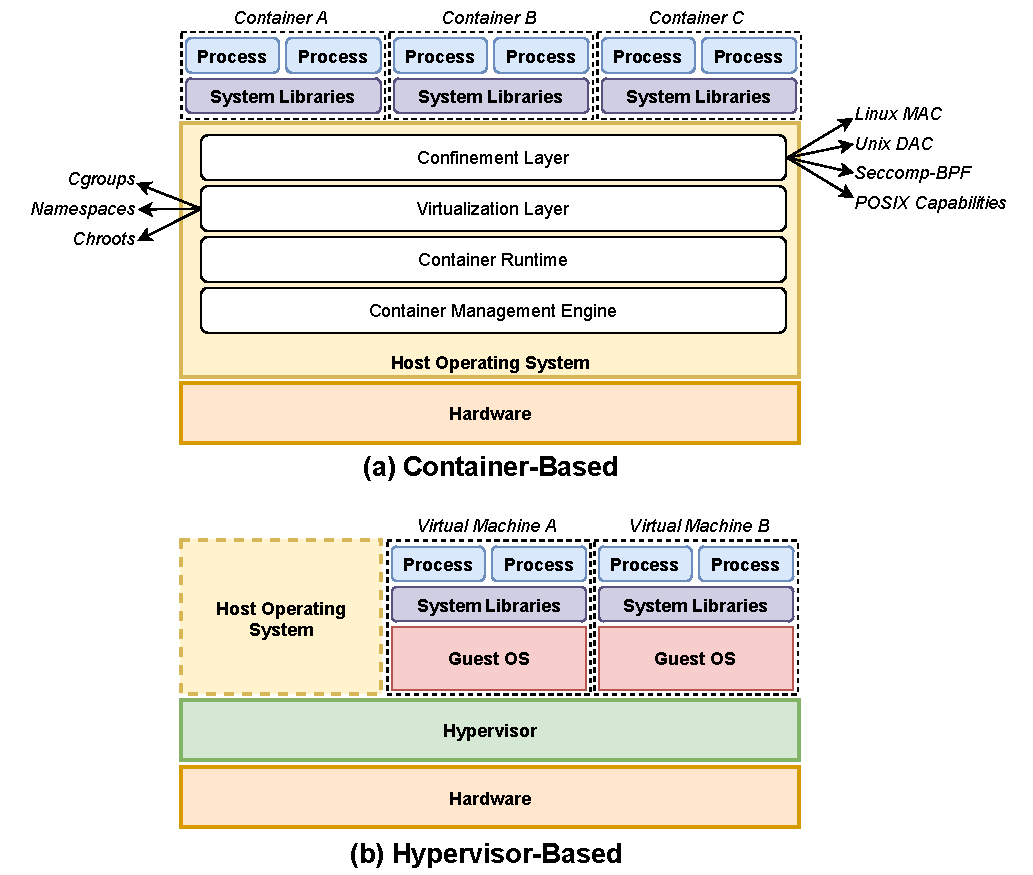
\includegraphics[width=1\linewidth]{figs/background/virtualization.pdf}
  \caption[A comparison of virtual machine and container architectures]{
    A comparison of virtual machine and container
    architectures~\cite{sultan2019_container_security, eder2016_hypervisor_container}.
    Containers \textbf{(a)} achieve virtualization using a thin layer provided by the host
    \gls{os} itself. They share the underlying operating system kernel and resources,
    requiring no guest \gls{os}. A hypervisor \textbf{(b)} virtualizes and controls the
    underlying hardware directly, but requires full guest operating systems on top of the
    virtualization layer.
  }\label{fig:virt}
\end{figure}



\subsection{Container Security}\label{ss:container-security-bg}

Due to the nature of containers as specialized process groups, any notion of container
security is necessarily tightly coupled with the underlying security primitives exposed by
the host operating system. These include the virtualization primitives discussed in
\Cref{s:virtualization}, and the confinement primitives discussed in
\Cref{s:process-security-model,s:security-extensions}. Whereas the primary attack surface
of a virtual machine is comprised of the interface exposed on top of hardware, the attack
surface of a container is comprised of the system calls that it uses to interact with the
host operating system kernel. Every system call is an opportunity to exploit a kernel
vulnerability; over-zealous resource-sharing is an opportunity to establish a covert
channel, or perform a confused deputy attack~\cite{hardy1988_confused_deputy} against
a privileged application. The cost to mount such attacks rapidly decreases as isolation
from the host operating system decreases.



\begin{figure}[htbp]
  \centering
  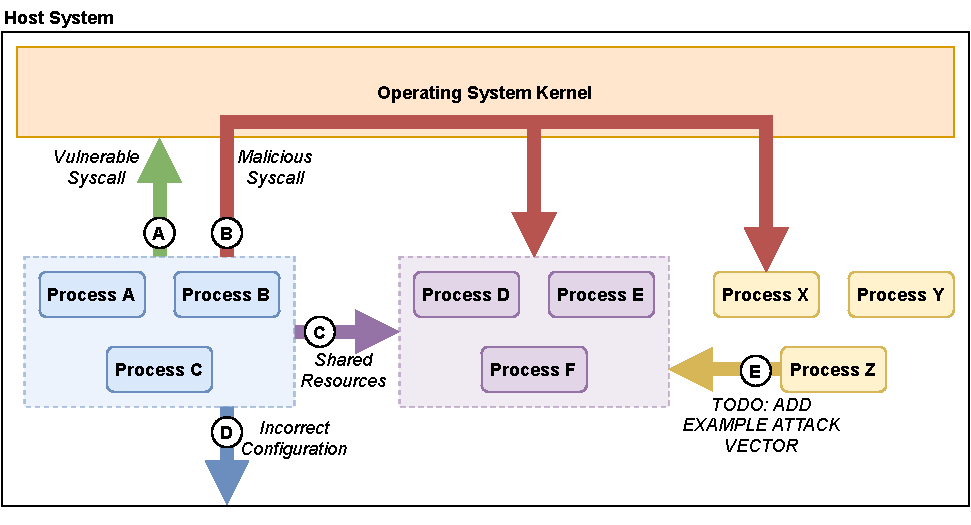
\includegraphics[width=0.8\linewidth]{figs/background/container_security.pdf}
  \caption[A sample threat model for container security]{
    A sample threat model for container security.
    \textbf{(A)} A container process attacks the host kernel directly.
    \textbf{(B)} A container process attacks another container process, passing through the host kernel's reference monitor.
    \textbf{(C)} A container process attacks a (privileged) host process, passing through the host kernel's reference monitor.
    \textbf{(D)} A host process attacks a container, passing through the host kernel's reference monitor.
  }\label{fig:containersec}
\end{figure}

\Cref{fig:containersec} depicts a high-level threat model for containers from the
perspective of the host operating system.  This model comprises a number of attack
vectors, each targeting a different part of the system. For instance, a malicious
container process can target the host kernel directly, providing input to a kernel
function through a system call (Item A in \Cref{fig:containersec}). This input can be
crafted to trigger a specific vulnerability in the host kernel, resulting in privilege
escalation, information disclosure, or denial of service.

A malicious container process can also target a process belonging to another container
(Item B in \Cref{fig:containersec}) or a (possibly privileged) host process (Item C in
\Cref{fig:containersec}). An attack could occur as a result of a misconfigured security
policy or some system resource shared by both processes. The end goal might be tampering
with the other process, or privilege escalation (for instance, via a Confused Deputy
attack~\cite{hardy1988_confused_deputy}). Finally, a host process can attack a container
process (Item D in \Cref{fig:containersec}). Goals in this case might include tampering
with a container belonging to another user of a multi-tenant system.

Not pictured in \Cref{fig:containersec} but important nonetheless is the case where
a process (containerized or otherwise) abuses a vulnerability in system hardware or
firmware (e.g.~a side channel attack on cache memory) to leak information about another
process (containerized or otherwise). Such attacks can totally bypass the operating
system's reference monitor and generally require trusted computing technologies or
hardware/software co-design to mitigate. As such, they are out of scope for this thesis.
Resource starvation attacks are also considered out of scope.



\subsubsection{Container Security in Industry}\label{sss:container-security-industry}

Existing container security on Linux is supported by a number of fundamental
virtualization and confinement mechanisms, covered in \Cref{s:process-security-model} and
\Cref{s:security-extensions}. Namespaces virtualize and limit the visibility of global
resource identifiers and cgroups virtualize and limit the available quantities of system
resources. Dropped POSIX capabilities allow the container to partition coarse-grained root
privileges into finer components. Seccomp-bpf filters limit the availability of system
calls to the container, while Linux \gls{mac} policies, enforced by an \gls{lsm} restrict
the container's access to system resources. Unix \gls{dac}, possibly accompanied by a new
user namespace, can limit the container's access as well, when properly configured.

\gls{lxc}~\cite{lxc_security} is a container runtime for Linux that directly exposes
low-level virtualization and confinement primitives. \gls{lxc} exposes namespaces and
cgroups to virtualize system resources and seccomp-bpf to filter system calls, reducing
the kernel's attack surface.

Docker~\cite{docker_security, bui2015_docker_analysis, combe2016_to_docker}, originally
based on \gls{lxc}, provides a high-level interface for creating, manipulating, and
running container images. Docker places containers in a new cgroup with sensible defaults
for resource virtualization. To isolate processes, the filesytem, and network interfaces,
Docker containers run in a new \gls{pid}, \gls{ipc}, mount, and net
namespace by default.  Similarly, Docker uses the \gls{uts} namespace for hostname
virtualization and the cgroup namespace to limit cgroup membership visibility. To
reduce the kernel's attack surface, Docker also includes a default seccomp-bpf profile
that blocks 51 system calls. Finally, Docker supports integration with the AppArmor
\gls{lsm} when it is enabled on the host, using a generic default profile that provides
modest protection~\cite{docker_apparmor, docker_default_apparmor}.

Unfortunately, Docker does not run in a new user namespace by default, making privilege
escalation from within a container significantly more likely~\cite{docker_security}.
However, it does offer the ability to opt-in to user namespace confinement with some
additional setup.  Docker also provides a \texttt{--privileged} flag which allows a user
to totally ignore all security defaults, essentially granting the container the same
access as a (often root-privileged) host process.



\subsubsection{Container Security in Academia}\label{sss:container-security-academia}

Sultan \etal~\cite{sultan2019_container_security} published a comprehensive review of
container security, including a threat model and comparison with full-virtualization
solutions like type I and type II hypervisors. Their work outlined four distinct cases and
presented a survey of existing security mechanisms targeting each case: (i)
a containerized attacking the container; (ii) a container attacking other containers;
(iii) a container attacking the host; and (iv) the host attacking a container. Their
recommendations included an increased adoption of trusted computing technologies to solve
case iv and that work towards a container-specific \gls{lsm} would be necessary to harden
against cases i--iii. \bpfcontain{}, one of the two research systems presented in this thesis,
represents a step towards such a container-specific \gls{lsm}.

Lin \etal~\cite{lin2018_container_security} presented a measurement study on container
security measures and attacks. They hand-crafted an exploit data set consisting of 233
exploits and used it to test the security defaults employed by Docker. Their findings
indicated that inter-dependence and mutual-influence among several disparate kernel
security mechanisms resulted in weaknesses in protection. Motivated by their findings,
they developed a simple kernel patch hardening the \texttt{commit\_creds()} function
against simple privilege escalation attacks mounted from containers.

Combe \etal~\cite{combe2016_to_docker} and Bui~\cite{bui2015_docker_analysis} presented
informal security analyses of Docker's default security configurations and Docker security
in general. Combe \etal~\cite{combe2016_to_docker} found that Docker configurations are
weak to supply-chain attacks involving malicious images and configurations on Docker Hub.
Additionally, they found that, while Docker's default configuration is relatively secure,
container misconfiguration, or the absence of security mechanisms such as AppArmor on the
host leaves the host vulnerable to attack. They also found that the default mandatory
access control policies employed by Docker were overly-permissive and far too generalized
to provide practical protection.

Bui~\cite{bui2015_docker_analysis} found that, while Docker does offer inadequate
protection against many sophisticated attacks, it still yielded security benefits over
running applications natively on the host. Bui recommends that containers be run under
virtual machines to add an additional layer of isolation from the host system. These
findings, however, demonstrate a lax attitude toward container security, opting to rely on
additional layers of indirection to provide real security guarantees and positing that at
least some protection is better than none at all.
Eder~\cite{eder2016_hypervisor_container} compared hypervisor- and container-based
virtualization and found that hypervisors are naturally more secure due to increased
levels of independence and isolation.

Babar \etal~\cite{babar2017_understanding}, and Mullinix
\etal~\cite{mullinix2020_security_measures} studied the container security mechanisms
underlying the Linux container infrastructure. Their findings separately indicate that
existing security mechanisms provided by the kernel are insufficient to offer full
protection from container vulnerabilities, particularly given the unique nature of the
attack surface exposed by the container running directly on the host operating system.

To address limitations imposed by container security defaults and alleviate concerns about
poor security practices in default configurations, many researchers have turned to
automatic policy generation~\cite{loukidis2018_dockersec, ghavamania2020_confine,
lei2017_speaker}.  Dockersec~\cite{loukidis2018_dockersec} uses a combination of static
analysis techniques on existing security profiles and a dynamic training process to
automatically infer AppArmor profiles for containers.  These inferred profiles provide
greater protection than the generic default profile since they are finer-grained and
tailored to the container's access patterns. In addition to generating \gls{mac} policy,
others have focused on generating seccomp-bpf policy to reduce the kernel's attack surface
from within a container. Confine~\cite{ghavamania2020_confine} uses static binary analysis
and library call instrumentation to generate seccomp-bpf policy for container images.
Their results showed that they were able to significantly reduce the attack surface for
kernel exploitation in many of the most popular Docker images.
SPEAKER~\cite{lei2017_speaker} partitions application containers into two distinct
phases\,---\,the setup and execution phase\,---\, and generates a unique seccomp-bpf
policy for each phase, enabling a tighter bound on confinement for each phase.

Others have focused on promoting self-confinement for containerized applications. Sun
\etal~\cite{sun2018_security_namespace} proposed the inclusion of a security namespace
into the kernel, allowing individual containers to load their own independent \gls{mac}
policy. This approach enables a clear separation of concerns between host policy and
container policy, and provides a clear path toward unprivileged self-confinement. The
approach is also generic enough to enable the use of alternative \gls{lsm}-based
confinement solutions on a per-container basis. \bpfcontain{}, for instance, might work
cooperatively with security namespaces for more efficient per-container confinement.

Vulnerability analysis of container images~\cite{shu2017_image_vuln, kwon2020_divds,
brady2020_docker_cloud} can be an effective technique for identifying weaknesses in
container deployments. Unlike policy generation, vulnerability analysis is a strictly
informative tool, allowing security experts to identify weaknesses in production
deployments and fix them. Shu \etal~\cite{shu2017_image_vuln} presented DIVA, a framework
for analyzing vulnerabilities in images deployed from Docker Hub. They aggregated data
from over 350,000 container images and found that images contained an average of 180
security vulnerabilities. Kwon and Lee~\cite{kwon2020_divds} proposed DIVDS, which
extends prior work by providing an interface to compare and allow specific image
vulnerabilities.  Brady \etal~\cite{brady2020_docker_cloud} applied similar vulnerability
scanning techniques to a continuous integration pipeline, flagging and fixing image
vulnerabilities during development.

\gls{ebpf} is seeing increasing prominence within the container security space. Besides
\bpfbox{} (c.f.\ \Cref{c:bpfbox}) and \bpfcontain{} (c.f.\ \Cref{c:bpfcontain}), other
projects have arisen over the past few years, albeit with a general focus on observability
rather than policy enforcement. Tracee~\cite{tracee} is a container observability tool
developed by Aqua Security that can watch system calls made by a container, along with
other security-sensitive events, and generate audit logs for further analysis.
Cilium~\cite{cilium} is a popular security daemon for the Kubernetes container
orchestration framework, with a focus on network security for distributed container
deployments. Cilium provides observability metrics through a configurable audit framework
and allows the end user to define network policy for telemetry, performance optimization,
and security.

\section{Extended BPF}\label{s:ebpf-bg}

\gls{ebpf} stands for \enquote{Extended \gls{bpf}}, though in reality it has very
little to do with Berkeley, packets, or filtering in its current
form~\cite{gregg2019_bpf}. In a nutshell, \gls{ebpf} is a Linux kernel technology that supports
dynamic system monitoring through the attachment of special \enquote{hooks} called \gls{bpf}
programs to specific kernel interfaces and userspace functions. In recent years, \gls{ebpf}'s
role has expanded, providing an interface to make extensions to the kernel as well as the
classic monitoring use case. In this section, we discuss the origins of \gls{ebpf}, its
components and how they work, its applications under the Linux kernel, and how it has
evolved over time.

\subsection{Origins of BPF\@: Efficient Packet Filtering and Beyond}\label{ss:origins-of-bpf-bg}

The original Berkeley Packet Filter, hereafter referred to as \gls{cbpf}\footnote{Throughout the rest of this thesis, we refer to extended \gls{bpf} using the terms
\enquote{\gls{ebpf}} and \enquote{\gls{bpf}} interchangeably. This is a matter of established
convention within the \gls{ebpf} community. Classic \gls{bpf} will be explicitly referred to by its
full name or the \gls{cbpf} acronym.}, arose out of a need to implement a more efficient packet
filtering mechanism for BSD Unix.  McCanne and Jacobson~\cite{mccanne1993_bpf} published
their work on \gls{cbpf} in 1993, marking an improvement over existing mechanisms in a number of
ways. Many of the reasons why classic \gls{bpf} was such an improvement over the status quo are
still relevant when discussing \textit{\gls{ebpf}}, and so we will briefly cover them here as
well.

In essence, classic \gls{bpf} is a \textit{register virtual machine} designed to take packets as
input and produce \textit{filtering decisions} as output. These filtering decisions could
then used to make decisions about whether a packet should be passed down to a more complex
pipeline for further analysis. The key insight behind \gls{cbpf} is that these filtering
decisions could be made more efficiently in \textit{kernelspace}, the part of the
operating system that runs in protection ring 0\footnote{Code that runs in ring 0 is said
to run with \textit{supervisor privileges} and is able to access all system memory. Ring
0 is the highest level of memory protection provided by the \gls{cpu}~\cite{jaeger2008_os_security}.}
and which is most commonly associated with any parts of the operating system that do not
run in \textit{userland} (i.e.\ the context of an ordinary user process). This provides
a considerable performance advantage over conventional approaches to network monitoring.
A typical network monitor runs in \textit{userspace}, meaning that packets need to be
copied over from kernelspace before they can be properly analyzed. This is an expensive
operation, requiring several context switches and potentially sleeping in the event of
a page fault~\cite{mccanne1993_bpf}.  By applying filtering logic in the kernel, this
expensive copying could be skipped for packets that would be discarded or ignored by the
network monitor anyway.

\begin{figure}[htbp]
  \centering
  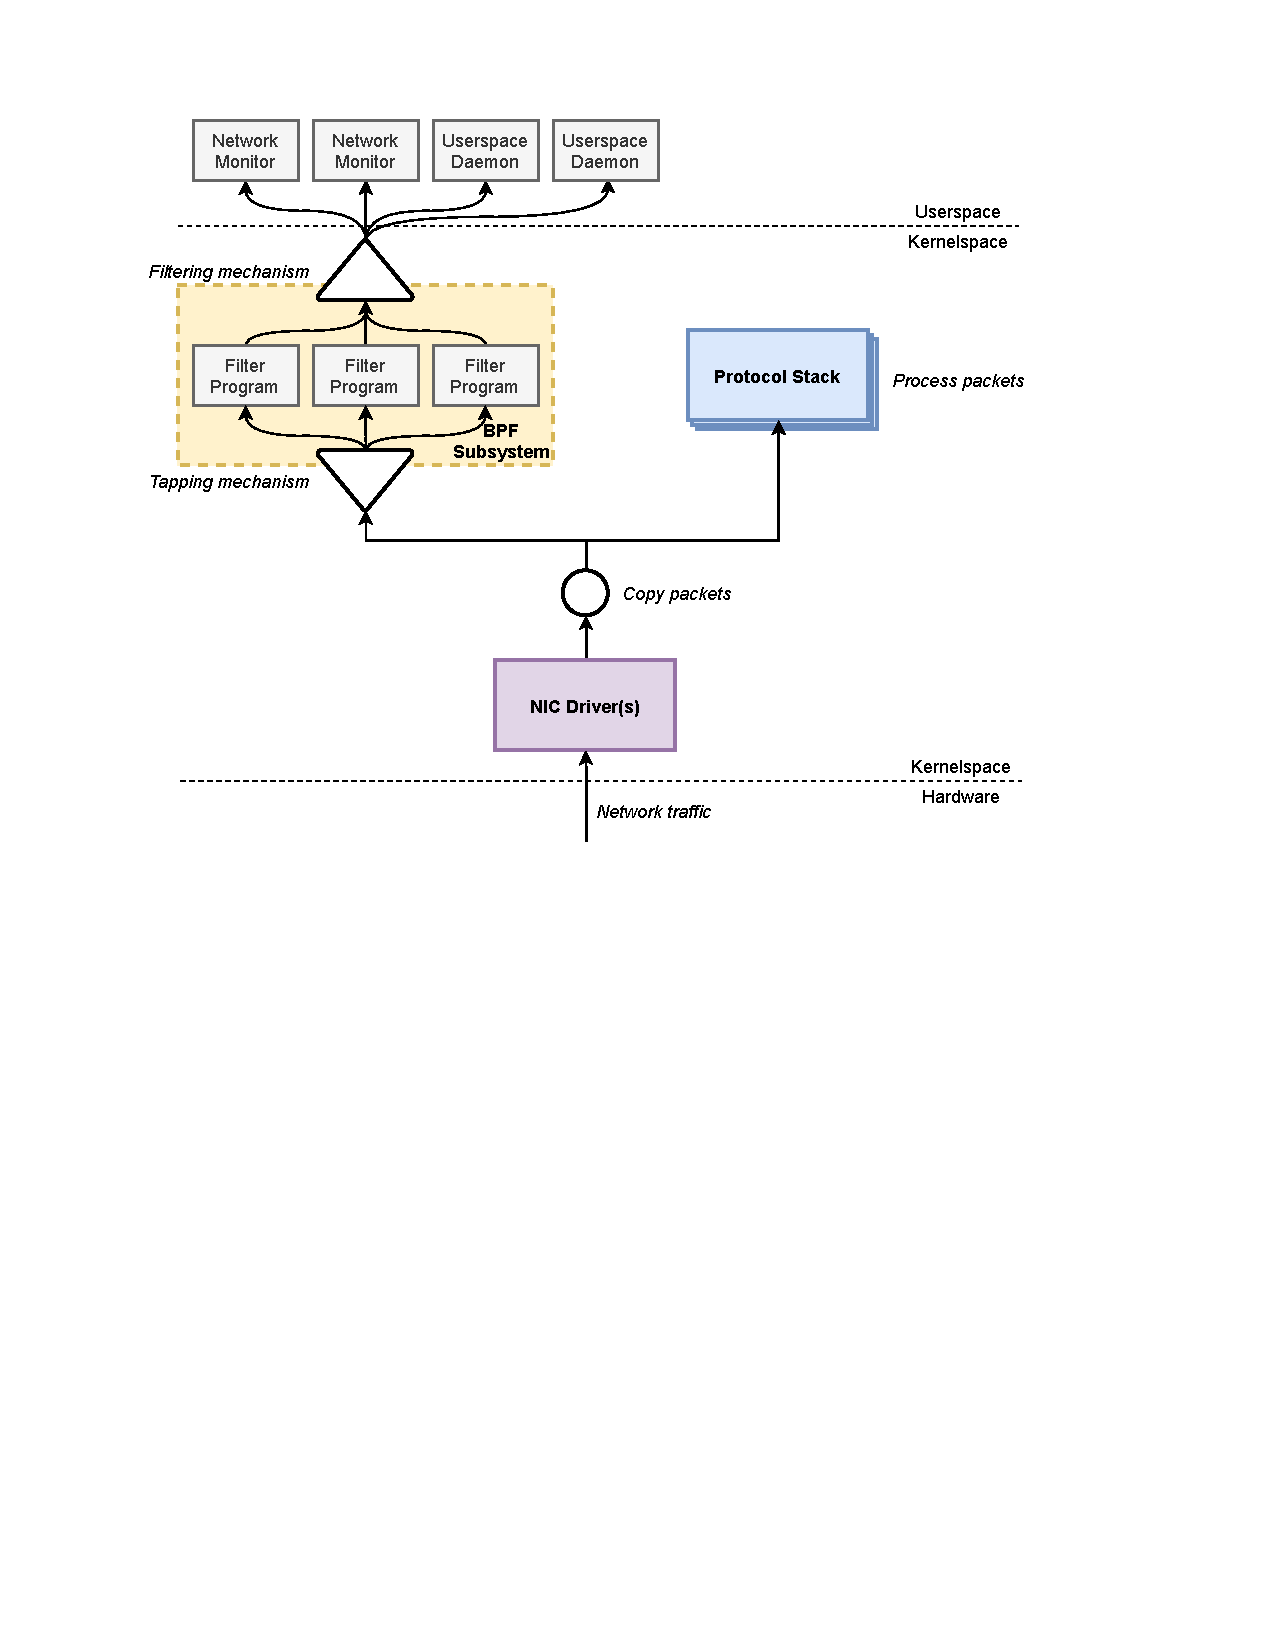
\includegraphics[width=0.8\linewidth]{figs/background/classic-bpf.pdf}
  \caption[The classic BPF architecture]{
    The classic \gls{bpf} architecture. Adapted from McCanne and Jacobson~\cite{mccanne1993_bpf}.
  }\label{fig:classic-bpf}
\end{figure}

Classic \gls{bpf} can be divided into two major components: a \textit{tap} mechanism and a set
of one or more \textit{filter} programs. The cBPF architecture is depicted in
\Cref{fig:classic-bpf}. \gls{cbpf} programs are expressed as a control-flow graph (CFG)
over a set of abstract registers, backed by physical registers on the \gls{cpu}. The tap
mechanism hooks into packets as they enter the networking stack, copying and forwarding
them to the filters. At runtime, the filter programs walk their control-flow graph, taking
the forwarded packets as input. As output, they return a filtering decision which controls
whether or not the packet should be forwarded to userspace~\cite{mccanne1993_bpf}.

Since its original introduction in 1993, classic \gls{bpf} has since been ported to
a number of Unix-like operating systems, including Linux~\cite{linux_bpf},
OpenBSD~\cite{openbsd_bpf}, and FreeBSD~\cite{freebsd_bpf}. Classic \gls{bpf} forms the
backbone of widely used traffic monitoring tools, most notably tcpdump~\cite{tcpdump,
mccanne1993_bpf}. In Linux, the \texttt{seccomp(2)} system
call~\cite{anderson2017_comparison} was enhanced to include classic \gls{bpf} filters,
allowing a user process to use classic \gls{bpf} programs to define allowlists and
denylists of system calls (c.f.\ \Cref{sss:seccomp}).

In 2014, Alexei Starovoitov and Daniel Borkmann~\cite{starovoitov2014_ebpf} first proposed
a total overhaul of the Linux \gls{bpf} engine. Their proposal, dubbed \gls{ebpf}, expanded the
classic \gls{bpf} execution model into a full-fledged virtual instruction set. In particular,
the extensions included a 512 byte stack, 11 registers (10 of which are general-purpose),
the ability to call a set of allowlisted kernel helper functions, the ability to attach
programs to a variety of system events, specialized data structures (called \gls{bpf} maps) to
store and share data at runtime, and an in-kernel verification engine to check for program
safety. At runtime, programs can be dynamically attached to system events and are
just-in-time compiled into the native instruction set.  \Cref{fig:extended-bpf} depicts
the \gls{ebpf} architecture in detail. The reader is encouraged to compare this with the classic
BPF architecture, depicted in \Cref{fig:classic-bpf}.

Dtrace~\cite{cantrill2004_dtrace, gregg2001_dtrace} served as an early inspiration for the
design of \gls{ebpf} and related tooling. The original Dtrace model was to make low-level
systems tracing available to end users by exporting a simple tracing language (called D)
and supporting upstream hooking of kernel functions using this language. \gls{ebpf}
implements a superset of Dtrace's original functionality, enabling userspace applications
to hook into the kernel and other userspace applications, attaching bytecode programs to
be run as callbacks.  Userspace \gls{ebpf} tooling then simplifies the process of writing
\gls{ebpf} programs by introducing increasingly high-level layers of abstraction.

\begin{figure}[htbp]
  \centering
  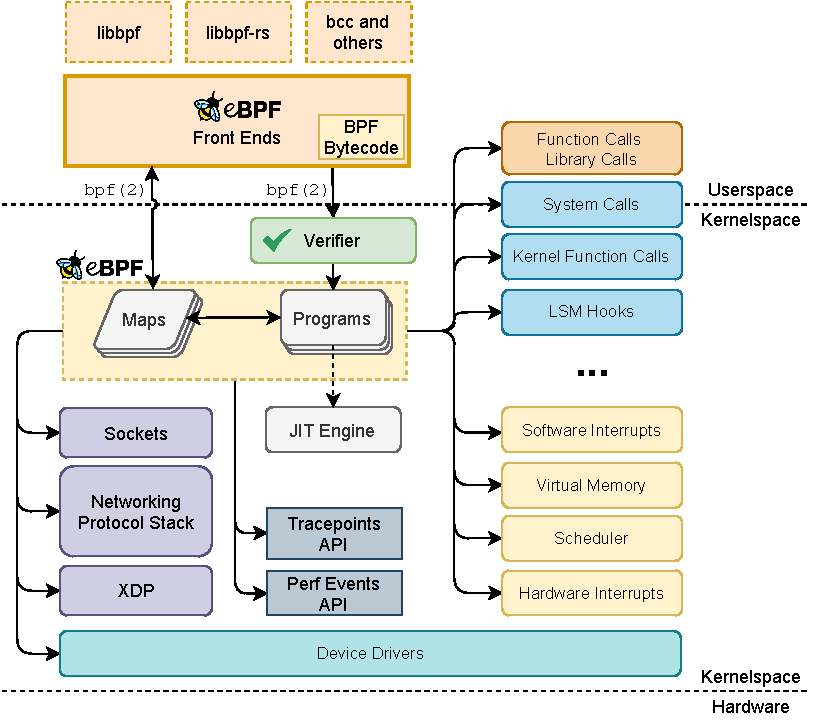
\includegraphics[width=0.8\linewidth]{figs/background/ebpf.pdf}
  \caption[The extended BPF architecture]{The extended \gls{bpf} architecture. Unlike classic
  \gls{bpf}, \gls{ebpf} programs are \gls{jit} compiled to the native instruction set, share data using
  specialized map data structures, and can be attached to many different kinds of system
  events. Programs can share data with each other and with the controlling userspace
  process using specialized map data structures. All \gls{ebpf} bytecode goes through
  a verification step before it can be loaded into the kernel.}\label{fig:extended-bpf}
\end{figure}

While modern \gls{ebpf} has very little to do with the execution model of its older cousin, some
of the properties that made classic \gls{bpf} so performant still hold true today. In
particular, to notion of aggregating and processing data in kernelspace before
(optionally) handing it off to userspace is a key aspect of classic \gls{bpf} that has carried
over to \gls{ebpf}. What this means in practice is that \gls{ebpf} programs can be used to implement
very efficient monitoring software, harnessing the performance benefits of a pure
kernelspace implementation while maintaining the flexibility of a userspace
implementation.

\subsection{eBPF Programs}\label{ss:bpf-programs-bg}

\gls{ebpf} programs are expressed in a virtual RISC machine language called \gls{bpf}
bytecode.  While it is technically possible to write \gls{bpf} bytecode by hand, programs
are most often compiled from a restricted subset of the C programming
language\footnote{Other languages may eventually be used to write \gls{ebpf} programs as
well.  For instance, an experimental Rust \gls{ebpf} target has recently been merged into
the Rust compiler~\cite{decina2021_bpf_rust}. The important distinction here is that the
set of all possible \gls{ebpf} programs is a strict subset of the set of all possible
programs.} using the LLVM toolchain. Programs can be loaded and attached to system events
using the \texttt{bpf(2)} system call, at which point control passes to the \gls{ebpf}
verifier, which checks the programs to make sure they satisfy a set of safety
constraints~\cite{starovoitov2014_ebpf, gregg2019_bpf}.

In particular, \gls{ebpf} programs must consist of fewer than 1 million \gls{bpf}
instructions and must not call into any kernel functions outside of the allowlisted
helpers. The program is also constrained to a 512 byte stack size; any additional memory
required by the program must come from an \gls{ebpf} map (c.f.\ \Cref{ss:bpf-maps-bg}). For
safety, memory accesses into allocated buffers must be properly bounds checked, pointers
must be null checked before dereferencing, and any access to external memory
(e.g.\ belonging to userspace programs or to the kernel itself) must be read only. Since
\gls{ebpf} programs must provably terminate, no back-edges are permitted in their control
flow and all loops must be bounded by some fixed constant $i$ iterations.

To guard against data races, \gls{ebpf} programs always hold the kernel's RCU (read-copy-update)
lock while executing, gated by the \texttt{bpf\_prog\_enter} and \texttt{bpf\_prog\_exit}
functions in the kernel. In simple terms, the RCU lock allows concurrent reads, except in
the presence of updates, optimizing for read-mostly workloads (i.e.\ precisely the sort of
workload \gls{ebpf} is designed for)~\cite{mckenney2007_rcu}. This implicitly enables \gls{bpf}
programs to read from many common kernel data structures without fear of data races and
simultaneously protects reads and updates to \gls{ebpf} maps, at a slight (albeit reasonable)
performance penalty~\cite{mckenney2007_rcu}. In addition to holding the RCU lock, \gls{ebpf}
programs are not considered \textit{preemptable} by default. In practice, this means that
\gls{ebpf} programs cannot sleep and must run to termination on their assigned core. This
property, while useful in many circumstances, enforces undesirable limitations on \gls{ebpf}
helpers, since it precludes any functionality that may cause the program to sleep (e.g.\ a
page fault). To account for use cases where sleeping is unavoidable, Linux 5.10 introduced
sleepable versions of some \gls{ebpf} program types~\cite{starovoitov2020_sleepable}.

Once loaded into the kernel, \gls{ebpf} programs are represented as \gls{bpf} objects, each with its
own reference count. Loading a \gls{bpf} program and attaching it to a system event increments
the reference count, while detaching and unloading the program decrements the reference
count. The kernel also exposes a special filesystem, \textit{bpffs}, which allows \gls{bpf}
programs to be pinned. This also increments the reference count, allowing an attached
program to outlive its controlling process (i.e.\ the process that loaded and attached
it)~\cite{gregg2019_bpf}.

\subsubsection*{Working with the Verifier}

In practice, the restrictions imposed by the verifier mean that \gls{ebpf} programs are not
\textit{Turing complete}~\cite{gregg2019_bpf}.  This property is required, given that the
halting problem (i.e.\ the decidability of program termination) is known to be unsolvable
for Turing-complete programs. This notion of Turing-incompleteness means that the set of
all possible \gls{ebpf} programs is a strict subset of the set of all possible C programs. While
these limitations help to ensure program safety, they also naturally restrict some
operations which \textit{may} be safe but are not strictly verifiable. To overcome the
limitations imposed by the verifier and achieve this safe-yet-unverifiable behaviour, \gls{ebpf}
programmers have a few tools in their arsenal. For instance, a specific set of allowlisted
kernel helpers offers the ability to call into specific kernel functions, bypassing the
limitations imposed by the \gls{ebpf} verifier. As a simple example, the
\texttt{bpf\_probe\_write\_user()} helper allows an \gls{ebpf} program to write to a userspace
memory address, bypassing the read-only restrictions imposed by the verifier. While these
allowlisted helpers operate in a \textit{mostly} unrestricted context, their usage
\textit{is} restricted at the function call boundary, ensuring that the \gls{ebpf} program obeys
the safety contract specified by the helper function.  Another common design pattern is
using a dummy \gls{ebpf} map as a scratch buffer to reserve a larger amount of memory for the
\gls{ebpf} program.  Since \gls{ebpf} programs cannot sleep~\cite{gregg2019_bpf}, dynamic memory
allocation within the \gls{bpf} context is impossible. These dummy maps offer a way to access
additional memory from a pool reserved at the time the map was loaded into the kernel.

\subsubsection*{eBPF Program Types and Use Cases}

Each \gls{ebpf} program has a specific \textit{program type}, which determines both the
set of system events to which the program can attach and the set of allowed kernel helpers
that can be called from within the program context. Each program type roughly corresponds
with a distinct \gls{ebpf} use case. For the purposes of this thesis, we will primarily be
dealing with \textit{\gls{lsm} probes}, \textit{raw tracepoints},
\textit{uprobes/uretprobes}, \textit{kprobes/kretprobes}, \textit{fentry/fexit probes},
and \textit{\gls{usdt} probes} as they form the basis of \bpfbox{} and \bpfcontain{}'s
kernelspace implementations. \Cref{tab:program-types} summarizes the relevant program
types and their properties.

\begingroup\small
\begin{longtable}[c]{lp{4.2in}}
\caption[A selection of relevant eBPF program types for \bpfbox{} and \bpfcontain{}~\cite{gregg2019_bpf}]{A selection of relevant \gls{ebpf} program types for \bpfbox{} and \bpfcontain{}.}\label{tab:program-types}\\
  \toprule
  Program Type & Description\\
  \midrule
  \textit{\gls{lsm} Probes}    & \gls{lsm} probes~\cite{singh2019_krsi} attach to the kernel's \gls{lsm} hooks and can be used to audit security events and make policy decisions.\\
  \textit{Raw Tracepoints}     & Raw tracepoint programs attach to a stable tracing interface exposed by the Linux kernel. Tracepoints are considered a stable \gls{api} but are more limiting than alternatives such as Kprobes or Fentry probes.\\
  \textit{Kprobes/Kretprobes}  & Kprobe programs can attach to any kernel function, by replacing the function with a trap into the \gls{bpf} program. The \gls{bpf} program has read-only access to the function arguments. Kretprobes work in the same way, but handle function returns instead of function calls.\\
  \textit{Fentry/Fexit Probes} & A more efficient version of Kprobes and Kretprobes that directly trampolines into the \gls{bpf} program instead of trapping. These programs can also be used to modify the return value of specifically allowlisted kernel functions (e.g.\ system call implementations).\\
  \textit{Uprobes/Uretprobes}  & The userspace equivalent of Kprobes and Kretprobes.\\
  \textit{\glsentryshort{usdt} Probes}  & A statically defined version of uprobes and uretprobes. Application developers may place these at strategic points within an application in order to add explicit support for userspace tracing at compile-time.\\
  \bottomrule
\end{longtable}
\endgroup

\subsubsection*{LSM Probes: Making Security Decisions with eBPF}

It is worth spending more time focusing specifically on \gls{lsm} probes, as these are used
extensively in \bpfbox{} and \bpfcontain{} to enforce policy over security-sensitive
events. Introduced by KP Singh in his \gls{krsi}
patch~\cite{singh2019_krsi}, \gls{lsm} probes define a canonical framework for attaching \gls{ebpf}
programs to the Linux kernel's \gls{lsm} security hooks (c.f.\ \Cref{ss:mac}). Unlike
traditional \gls{lsm}s which are implemented as static kernel modules, \gls{lsm} probes are
\textit{dynamically attachable}, meaning that access control and audit policy can be adjusted at
runtime, simply by loading a new \gls{ebpf} program.  \Cref{fig:bpf-lsm} depicts how \gls{lsm} probes
integrate with the \gls{lsm} framework.

\begin{figure}[htbp]
  \centering
  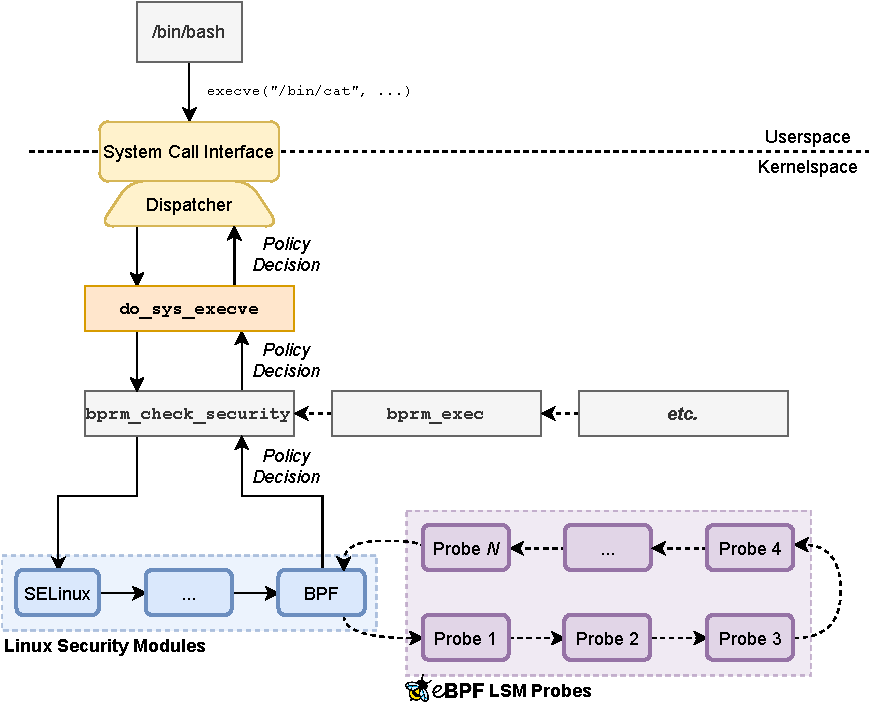
\includegraphics[width=0.8\linewidth]{figs/background/bpf-lsm.pdf}
  \caption[How eBPF LSM probes make policy decisions]{A simplified example of how \gls{ebpf} \gls{lsm} probes make policy decisions. Privileged userspace processes can attach one or more \gls{lsm} probes to a given hook. When a userspace process requests a privileged operation, the kernel implicitly calls into the corresponding \gls{lsm} hooks, which in turn invoke the logic associated with each \gls{lsm}. A shim \gls{lsm} is responsible for invoking each \gls{lsm} probe, and any resulting policy decisions are taken together to arrive at a final decision. As with ordinary \gls{lsm}s, the final decision is consensus-based. That is, if \textit{any \gls{lsm}s} or \textit{any \gls{bpf} \gls{lsm} probes} disagree on a policy decision, the privileged operation is denied.}\label{fig:bpf-lsm}
\end{figure}

Each \gls{lsm} probe can be attached to one or more \gls{lsm} hooks defined in the kernel.
When the hook fires (i.e.\ when a task requests a privileged operation form the kernel),
every attached probe fires as part of the normal \gls{lsm} pipeline. The body of the
\gls{bpf} program defines filtering and audit logic, optionally accessing maps to store
and query persistent state. The \gls{bpf} program then returns a security decision about
whether the requested operation should be allowed or denied.  In order for an operation to
be allowed, \textit{all} other \gls{lsm}s and \gls{lsm} probes must agree on the policy
decision and ordinary security checks performed by the operating system must also succeed.
In other words, it is not possible to grant additional privileges using an \gls{lsm}
probe.

Owing to the properties discussed earlier in this section, \gls{ebpf} confers a natural
flexibility to \gls{lsm} probes quite unlike that of traditional \gls{lsm}-based security
frameworks.  In particular, \gls{lsm} probes can be attached at runtime and can cooperate
with other \gls{ebpf} program types using \gls{ebpf} maps (c.f.\ \Cref{ss:bpf-maps-bg}).
This notion of cooperating programs presents an opportunity to design modular policy
enforcement mechanisms that operate beyond the scope of the \gls{lsm} hooks framework
itself.  Another key advantage of \gls{lsm} probes over traditional \gls{lsm}s lies in
their adoptability.  While industry actors may be understandably reluctant to adopt
\enquote{yet another out-of-tree \gls{lsm}}, a security mechanism based on \gls{ebpf} does
not carry the same technical baggage.  \gls{ebpf} programs are safe to use in production
and can be deployed at runtime on an unmodified kernel.  This makes \gls{ebpf}
a particularly attractive target for developing new security solutions.

\subsection{eBPF Maps}\label{ss:bpf-maps-bg}

\gls{ebpf} maps serve as both a runtime data store for \gls{ebpf} programs and the
canonical method of communication between different \gls{ebpf} programs and userspace
applications. Like \gls{ebpf} programs, maps can be pinned to \textit{bpffs} to increment
their reference count in the kernel.  Concurrent access to \gls{ebpf} maps from within
kernelspace is protected by an implicit RCU lock, and a spinlock concurrency primitive is
exposed via a helper function to guard map accesses between kernelspace and userspace.
From the \gls{ebpf} side, maps can be accessed using a set of provided helper functions.
Userspace applications can access maps using the \texttt{bpf(2)} system call or through
direct memory mapping (only available for arrays) via
\texttt{mmap(2)~\cite{gregg2019_bpf}}. While many \gls{ebpf} maps are designed to be
generic, others are highly specialized for specific use cases. \bpfcontain{} and \bpfbox{}
make use of several \gls{ebpf} map types (see \Cref{tab:map-types}.

\begingroup\footnotesize
\begin{longtable}[c]{lp{3.9in}}
\caption[A selection of relevant eBPF map types for \bpfbox{} and \bpfcontain{}~\cite{gregg2019_bpf}]{A selection of relevant \gls{ebpf} map types for \bpfbox{} and \bpfcontain{}.}\label{tab:map-types}\\
  \toprule
  Map Type & Description\\
  \midrule
  \textit{\gls{bpf} Hashmap}           & A key-value hashmap. Keys and values can be arbitrary data structures.\\
  \textit{\gls{bpf} Array}             & A fixed-size array with integer indices. Values can be arbitrary data structures.\\
  \textit{\gls{bpf} Array/Map of Maps} & A \gls{bpf} array or map that stores handles into \textit{other maps}.\\
  \textit{\gls{bpf} Per-\glsentryshort{cpu} Array/Map} & Like a \gls{bpf} hashmap or \gls{bpf} array but with a separate copy per logical \glsentryshort{cpu}\@. This enables concurrent access across \glsentryshortpl{cpu}, but without synchronization.\\
  \textit{\gls{bpf} Local Storage}     & A dummy \gls{bpf} map that provides a handle into local storage for a given kernel data structure. For instance, task local storage provides storage per task struct. Values can be arbitrary data structures.\\
  \textit{\gls{bpf} Ringbuf}           & A concurrent circular buffer that passes event handles from kernelspace to userspace. To communicate, \gls{ebpf} programs submit events and userspace applications poll events.\\
  \bottomrule
\end{longtable}
\endgroup

\subsection{Userspace Front Ends}\label{ss:bpf-userspace}

Although \gls{ebpf} programs and maps can exist on their own after being pinned to
\textit{bpffs}, the more common approach is to manage their lifetime using a controlling
process. Userspace applications implementing such a controlling process typically use an
\gls{ebpf} front-end framework to facilitate loading and interacting with programs and maps.
A number of such front ends exist~\cite{gobpf, bcc, libbpf, libbpf-rs, libbpfgo,
cilium-ebpf, redbpf}, some more practical than others.
\textit{bcc}~\cite{bcc} was the first \gls{ebpf} framework to offer high-level userspace tooling
around \gls{ebpf}, providing an LLVM backend for compiling \gls{ebpf} programs and a Python library
for loading and interacting with them. \textit{libbpf}~\cite{libbpf} offers a pure
C alternative to bcc and has since been upstreamed into the Linux kernel.
\textit{libbpf-rs}~\cite{libbpf-rs} and \textit{libbpfgo}~\cite{libbpfgo} offer Rust
and Golang bindings for libbpf respectively. Other tooling~\cite{cilium-ebpf, redbpf}
bypasses libbpf entirely, providing fully native \gls{ebpf} bindings for Rust and Golang.

\subsubsection*{Libbpf and BPF CO-RE}

Among the myriad of userspace front ends available for \gls{ebpf}, libbpf stands out as the only
one with official upstream support from the Linux kernel. Recent improvements to libbpf
have solidified its position as the dominant framework. In particular, libbpf supports
a new way of compiling and loading \gls{bpf} programs into the kernel, \gls{bpf}
\gls{core}~\cite{gregg2020_core, nakryiko2020_core}. \gls{bpf} \gls{core} uses \gls{btf}
debugging information exposed by the kernel, along with load-time relocation logic to
support loading the same compiled \gls{ebpf} bytecode across multiple target kernels.

With libbpf and \gls{core}, \gls{ebpf} programs can now be compiled once and run on any target kernel
that supports the required \gls{bpf} features. This provides a powerful advantage over other
\gls{ebpf} frameworks and even alternatives to \gls{ebpf}, such as loadable kernel modules. A \gls{core}
program that runs on one kernel will be guaranteed to run on another of the same version
or higher, barring any \gls{api} incompatibilities like changes in a hooked function signature.
Such incompatibilities can be resolved with the use of built-in kernel configuration
checks.

\bpfcontain{} (c.f.\ \Cref{c:bpfcontain}) leverages libbpf and \gls{core} through libbpf-rs, the
canonical Rust bindings for libbpf, providing adoptability advantages over the original
\bpfbox{} prototype (c.f.\ \Cref{c:bpfbox}), which uses bcc.

\subsection{Comparing eBPF with Loadable Kernel Modules}\label{ss:bpf-vs-modules}

Before \gls{ebpf}, the primary means of modifying the Linux kernel at runtime was through the
use of \textit{loadable kernel modules}~\cite{corbet1998_device_drivers}. A kernel module
can be thought of as a discrete bundle of code that can be loaded into the kernel (or
compiled into its binary image). Like other kernel code, including \gls{ebpf}, modules are
event-based and run in ring 0, responding to and handling system events as they occur.
Since kernel modules and \gls{ebpf} can serve similar (but not strictly equivalent) purposes,
comparing the two can offer some insight about how they differ and which technology is
better fit for a specific purpose.

At a first approximation, \gls{ebpf} differs from kernel modules in the following meaningful ways~\cite{gregg2019_bpf}:
\begin{enumerate}
  \item \gls{ebpf} programs \textbf{must pass verification checks} before they can be loaded into the
  kernel. This verification step provides assurances about program safety. For instance, \gls{ebpf}
  programs are guaranteed not to deadlock the kernel, and are far less likely to suffer from
  memory safety issues. In contrast, misuse of kernel \gls{api}s in a kernel module can have dangerous
  implications for system safety and security.

  \item An implicit advantage provided by \gls{ebpf} is that \gls{bpf} programs can be \textbf{easier
  to reason about} than other kernel code. \gls{ebpf} abstracts away much of the complex
  functionality required to make kernel code operate correctly by providing implicit
  guarantees about program execution. Even helper functions, which offer functionality
  beyond the scope of verifiability, must obey a predetermined contract with the verifier
  in order to be considered safe. Thus, when an \gls{ebpf} program passes verification, there is
  a much higher likelihood that it will \enquote{just work.}

  \item \gls{ebpf} \textbf{exposes map-like data structures} to facilitate runtime data storage,
  communication between \gls{ebpf} programs, and communication with userspace applications. In
  the case of kernel modules, data structures often must be implemented by hand, taking
  great care not to introduce potential bugs or security vulnerabilities, particularly in
  the case of memory management. Communication with userspace from a kernel module might
  be done via netlink sockets, file operations, or similar
  means~\cite{corbet1998_device_drivers}. These modes of communication are often less
  streamlined and, in the case of file operations, must be implemented by hand, increasing
  the likelihood of programmer error.

  \item \gls{ebpf} programs are \textbf{not Turing-complete}. Intuitively, this means that
  the set of operations a kernel module can perform is a strict superset of \gls{ebpf}. While
  this may appear to be a hugely limiting factor, in practice \gls{ebpf} programs are often
  sufficient to implement sophisticated tracing, filtering, and policy enforcement logic.
  Where the verifier gets in the way, the programmer can reach for a number of helper
  functions provided by the kernel to achieve more complex behaviour.

  \item \gls{ebpf} is \textbf{not \textit{generally} suitable for implementing device drivers} or
  other complex functionality that requires ad-hoc access to various kernel facilities and
  write access to arbitrary memory locations. Where necessary, \gls{ebpf} helpers can be
  added to the kernel to perform more complex functionality from within a \gls{bpf}
  program. However, these helpers must be upstreamed in the kernel in order to be used,
  are limited to specific program types, and must obey a safety contract with the
  verifier.
\end{enumerate}

\begin{table}[!htb]
  \centering
  \caption[A high-level comparison between \glsentryshort{ebpf}, loadable kernel
  modules, and kernel patches]{
    A high-level comparison between \glsentryshort{ebpf}, loadable kernel modules, and
    kernel patches. \fullc{} = property satisfied; \halfc{} = property somewhat satisfied;
    \emptyc{} = property not satisfied.
  }\label{tab:ebpf-comparison}
  \begin{tabular}{lccccccp{4.8em}}
  \toprule
                       & \rot{45}{Loadable at Runtime} & \rot{45}{Verified Safety}
                       & \rot{45}{Easy Abstractions}   & \rot{45}{Cross-Boundary Data Structures}
                       & \rot{45}{Turing Complete}     & \rot{45}{Complex Functionality} & \\
  \midrule
  \glsentryshort{ebpf} & \fullc  & \fullc  & \fullc  & \fullc  & \emptyc & \halfc  & \\
  Kernel Modules       & \halfc  & \emptyc & \emptyc & \emptyc & \fullc  & \fullc  & \\
  Kernel Patches       & \emptyc & \emptyc & \emptyc & \emptyc & \fullc  & \fullc  & \\
  \bottomrule
  \end{tabular}
\end{table}

\Cref{tab:ebpf-comparison} presents a summary comparison of \gls{ebpf}, kernel modules,
and kernel patches as a means of running custom code in the kernel.  In summary,
\gls{ebpf} is useful for observability use cases, or cases in which the functional
requirements of the kernel code are not expected to be complex or might be expected to
change frequently. \gls{ebpf} programs and maps are particularly good at separation of
concerns, composability, and modularity. \gls{ebpf} maps facilitate easy communication
between kernelspace and userspace, and provide the ability to build relationships between
data from different program types. Kernel modules should be preferred for the
implementation of more complex kernel functionality, such as device drivers.

\chapter{The Confinement Problem}\label{c:confinement-problem}
\begin{comment}
  What is the original framing of the problem? It almost doesn't make sense to frame it as a system-wide problem. Because a process is useless if it's totally isolated from the rest of the system. Make processes isolated and poke some holes in this isolation.

  This is something that has been on the radar since the origin of multi-processing
  systems.  We can argue that one of the reasons it's never been solved has been because
  the problem is too broadly defined.

  One set of tehcnologies that has helped in this sense has been hypervisor-based
  virtualization. But this is subject to some fundamental concerns. Containers

  It's a reframing but it's also narrowing the scope
  A "scoping definition"? A "scoping reframing"?
  Applying it specifically to containers and virtualization
\end{comment}


Researchers have been studying confinement for decades~\cite{lampson1973_confinement}, and
have been designing and applying confinement primitives since the early days of
time-sharing computers and multi-tenant systems~\cite{shu2016_security_isolation_study}.
While many developments have been made in the mean time, the current confinement landscape
(particularly within the Linux ecosystem) suffers from fundamental flaws that culminate in
poor container security practices; this does not need to be so. This chapter presents
a critique of the current state of confinement on Linux, examines how confinement
primitives are applied to containers, and proposes a fundamental re-framing of the problem
to focus on complexity, adoptability, and suitability for container-specific applications.
In light of this re-framing, we consider design goals for \bpfbox{} and \bpfcontain{} and
present the threat model for confinement under these research systems.

\section{Rethinking the Virtualization Narrative}\label{s:cp-rethinking}

Hypervisor-backed virtualization is commonly considered more secure than
con\-tain\-er-based virtualization~\cite{sultan2019_container_security,
eder2016_hypervisor_container} (see \Cref{fig:container-hvm-security}). Intuitively, this
makes sense.  Containers run directly on the host operating system, whereas a virtual
machine runs on top of a hypervisor, separated by at least one layer of indirection from
the host system.  However, this intuition does not strictly stand up to scrutiny.
A virtual machine running on top of a hypervisor makes requests to the hypervisor's
\gls{api} (via hypercalls), in much the same way as a container running on a host
operating system makes requests to the kernel's \gls{api} (via system calls).
\Cref{fig:syscall-hypercall} illustrates this parity. In both cases, a vulnerable
interface into a more privileged component of the system is directly exposed to the
attacker.

\begin{figure}[htbp]
  \centering
  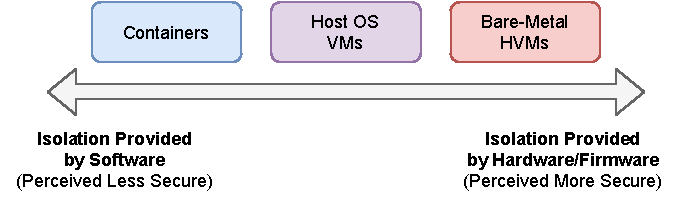
\includegraphics[width=0.8\linewidth]{figs/confinement-problem/security.pdf}
  \caption[Comparing the isolation and perceived security of containers and \glsentryshortpl{vm}]{
    Comparing the isolation and perceived security of containers and
    \glsentryshortpl{vm}. A boundary defined in hardware is often considered more rigid,
    whereas a software defined boundary is generally considered more malleable, and thus
    weaker. However, this need not be the case. A goal of this thesis is to reposition
    containers to be as secure, if not more secure, than hypervisor-based virtualization.
  }\label{fig:container-hvm-security}
\end{figure}

\begin{figure}[htbp]
  \centering
  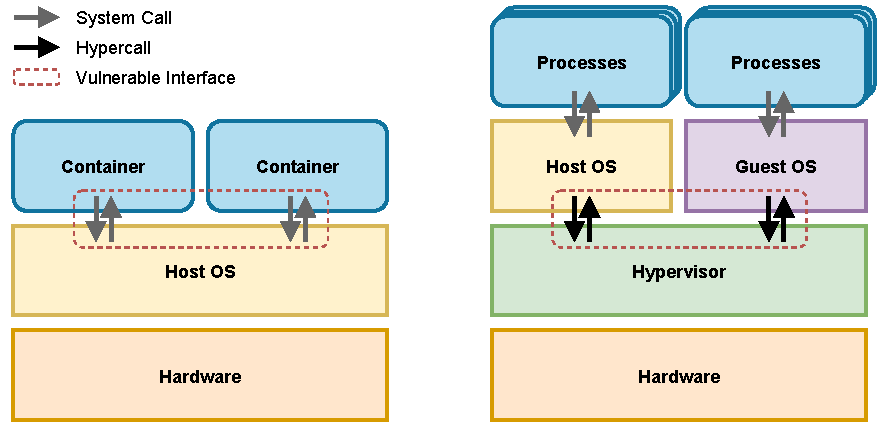
\includegraphics[width=0.8\linewidth]{figs/confinement-problem/syscall-hypercall.pdf}
  \caption[System calls and hypercalls as vulnerable interfaces]{
    System calls and hypercalls as vulnerable interfaces. Containers (which are really
    just process groups running on the host \gls{os}) make system calls to the
    more-privileged host \gls{os} kernel. Similarly, a guest operating system makes
    hypercalls to the more-privileged hypervisor. Both of these interfaces are ripe
    targets for a myriad of attacks, including privilege escalation and tampering with
    sensitive resources. This parity becomes particularly evident when we assume that an
    attacker has or is able to obtain control over the guest \gls{os}.
  }\label{fig:syscall-hypercall}
\end{figure}



In the case of virtual machines, security is an emergent phenomenon. The implicit
isolation provided by a virtual machine is purely a function of the semantic gap between
guest operating system, virtualized hardware, and physical hardware. Here, security is
intrinsically tied to functionality. Administrators poke holes in this isolation all the
time through shared filesystems, virtual network interfaces, and other virtual device
drivers. From there, it is up to the administrator to use conventional \gls{os} security
mechanisms (c.f.\ \Cref{s:process-security-model,s:security-extensions} in
\Cref{c:background}) such as filesystem access controls and network firewalls to lock down
the exposed interfaces.  A clear pattern emerges: first provision the resource, then secure
it, just as in an ordinary operating system (after all, a guest operating system
\textit{is} just an operating system). The end result of this process is a combination of
implicit isolation and additional \gls{os}-level security mechanisms: a form of
\textit{policy through mechanism}.

The central argument of this thesis is that there is no fundamental reason why containers
cannot be as\,---\,if not more\,---\,secure than virtual machines.  While it is true that
a containerized process is nothing more than a host process running under one or more
\gls{os}-level virtualization primitives, an operating system that provides and enforces
the right set of confinement primitives should be able to lock a container down in much
the same way that a hypervisor implicitly enforces isolation.  Unlike hypervisor-based
isolation, such a policy enforced by the operating system has the potential to be more
minimal, centralized, and accessible to end users. Further, we can attain a high level of
flexibility through a software-based enforcement mechanism, unencumbered by the
restrictions of a hardware-level interface.

The key to developing such an enforcement mechanism lies in defining a clear protection
boundary within the kernel and enforcing access across this boundary. Rather than
\textit{policy through mechanism}, this would be \textit{policy through exception}. Under
this model, the operating system enforces a clear protection boundary around the
container, and security policy then defines exceptions in this boundary, exposing
a minimal interface to the outside world.  Such an interface has the potential to be
\textit{far more minimal}  than that of a virtual machine, by taking advantage of the
fine-grained semantics exposed by the operating system.

However, the above depiction of container security does not match the current reality.
Existing container runtimes simply reuse confinement primitives exposed by the operating
system, combining multiple \gls{os}-level security mechanisms to secure specific system
resources.  This approach is neither simple nor unified, and results in increasingly
complex and verbose policies, inundated with the technical baggage associated with locking
down an entire operating system. Yet it is hard to fault the designers of container
runtimes for this design choice; a container runtime's job is to run containers, not to
implement new security mechanisms. Intuitively, it makes sense to reach for primitives
that already exist, regardless of the fact that these primitives may have been designed
for system-wide use cases, beyond individual processes or even process groups. Likewise,
the goal of this thesis is not to design a new container runtime\,---\,rather, it is to
implement the missing confinement mechanism that will enable our vision for container
security to become a reality.

Before we can address concrete goals for such a confinement mechanism
(c.f.\ \Cref{s:cp-design,s:cp-threat-model}), it is important to understand the fundamental
issues underlying the current state-of-the-art in Linux confinement and container
security. To that end, \Cref{s:cp-issues} outlines three main issues with current Linux
confinement primitives and \Cref{s:cp-containers} examines and critiques how container
runtimes apply these primitives in practice.














\section{Fundamental Issues with Linux Confinement}\label{s:cp-issues}

Here we identify three fundamental issues with the current state of Linux confinement and
contextualize them with examples from existing container and confinement frameworks. This
section serves to provide additional context for the container-specific issues discussed
in \Cref{s:cp-containers}, and the design goals for \bpfbox{} and \bpfcontain{}, discussed
in \Cref{s:cp-design}.

\begin{enumerate}[font=\bfseries]
  \item \label{i:problem-complexity} \textbf{Complexity, Interdependence, and Inflexibility.}
    Existing confinement primitives are overly complex and designed for use cases beyond
    simple process confinement. To achieve simple confinement, frameworks must abuse and
    recombine a number of existing primitives, each designed for a different use case.
    Namespaces~\cite{biederman2006_namespaces, linux_namespaces} were designed to
    virtualize resources; they do not provide confinement by themselves. To truly confine
    a process using namespaces, we need a way to account for namespace escapes.
    Cgroups~\cite{cgroups} similarly, were designed to virtualize the availability of
    quantifiable resources, not to directly confine. Unix
    \gls{dac}~\cite{jaeger2008_os_security, van_oorschot2020_tools_jewels} is far too
    coarse-grained and easy to bypass to be directly useful for confinement. POSIX
    capabilities~\cite{posix_capabilities} can be used to reduce overprivilege by
    partitioning root privileges, but these do not implement confinement by themselves.

    Seccomp-bpf~\cite{seccomp, edge2015_seccomp} works well to reduce the attack surface
    exposed by system calls, but writing classic \gls{bpf} filters is a complex and
    error-prone process. Fine-grained filtering quickly becomes untenable, particularly
    when considering race conditions when checking system call arguments and system call
    equivalence classes.  Linux \gls{mac} can be used to implement true confinement, but
    a typical \gls{lsm} like AppArmor~\cite{cowan2000_apparmor} or
    SELinux~\cite{smalley2001_selinux} is designed for use cases beyond simple sandboxing.
    These mechanisms are designed to implement and enforce system-wide \gls{mac} policy,
    not simple process-level confinement~\cite{belair2019_leveraging}. Further, major
    \glspl{lsm} are statically loaded and unstackable, meaning that end users must
    generally choose one major solution with little room to adjust enforcement at runtime.

    To implement confinement, sandboxing and containerization frameworks generally mix and
    match the aforementioned solutions\,---\,some of which were designed for confinement,
    some of which were not, and none of which were designed for \textit{simple,
    process-level} confinement. LXC, Docker, Snap, and others all combine namespaces,
    cgroups, capabilities, seccomp-bpf, and AppArmor/SELinux policy to achieve
    confinement. In the case of Snap, high-level abstractions in policy definition can
    simplify the process of policy authorship to a certain extent, but simple policies
    are still compiled down into thousands of lines of policy soup, spanning multiple
    confinement mechanisms. FreeBSD Jails and Solaris Zones take an alternate approach,
    enforcing a rigid protection boundary around the container, but with little flexibility
    for policy customization.

  \item \label{i:problem-unsuitability} \textbf{Unsuitability for Containers.}
    Existing Linux \gls{dac} and \gls{mac} is unsuitable for containers.
    \gls{lsm}-based \gls{mac} implementations like AppArmor and SELinux are
    designed to implement global, system-wide confinement policy; they are not designed
    for ad-hoc, process-level confinement~\cite{belair2019_leveraging}. Additionally,
    these \gls{lsm} implementations were not designed with containers in mind and thus
    do not consider container semantics in policy definition and enforcement. This lack
    of semantic awareness further complicates policy authorship for containers and
    forces the end user to make compromises between security and functionality.

    Sultan \etal~\cite{sultan2019_container_security} suggest that the container
    security community should move towards a container-specific \gls{lsm}
    implementation. Security namespaces, proposed by Sun
    \etal~\cite{sun2018_security_namespace} can be seen as a partial step toward solving
    this problem.  Under security namespaces, each container can load and use its own
    \gls{lsm} of choice, but these \glspl{lsm} would still be subject to many of the
    same aforementioned restrictions. That is, existing \glspl{lsm} are not designed
    with container semantics in mind. A truly container-specific \gls{lsm} could incorporate
    container semantics into policy enforcement for cleaner and more effective policies.

    \gls{uid} remapping under a new user namespace does help with the \gls{dac} case by
    remapping root to a non-root \gls{uid}, but this is only really helpful for limiting
    the power of root. Other limitations of \gls{dac} still apply. For instance,
    a world-readable file could still be used for information disclosure or
    a world-writable file could still be the target of data corruption. For such reasons,
    \gls{dac} alone appears to be fundamentally insufficient for true isolation between
    host and container. Thus, to achieve proper process-level confinement for containers,
    we need an \gls{lsm}-based solution that is aware of container semantics.

  \item \label{i:problem-adoptability} \textbf{Difficulty Adopting New Solutions.}
    Motivated by the inherent difficulties associated with the existing confinement space,
    academics are often tempted to propose new confinement solutions. Many try to solve
    the problem by simply recombining and reusing existing primitives in new and
    innovative ways.  However, these types of solutions generally are not really a step
    forward with respect to addressing the issues in items 1 and 2, since these are
    emergent properties inherent to the underlying confinement primitives themselves.

    In order to truly solve these fundamental issues, we need kernel support for new
    primitives. Unfortunately, this begets yet another fundamental issue: adding new
    solutions directly to the kernel is difficult, particularly from an adoptability
    standpoint. New kernel code can introduce bugs and security vulnerabilities. It needs
    to be thoroughly tested before it can be considered production ready. Paradoxically,
    the potential to introduce new security vulnerabilities can make the use of such novel
    primitives \textit{less} secure. Similarly, kernel bugs can introduce availability
    concerns in production systems, even when such bugs are not security critical. For
    these reasons, industry managers may be reluctant to adopt new, out-of-tree solutions
    based on loadable kernel modules, for example~\cite{gregg2019_bpf}.

Another adoptability concern arises when we consider \textit{container-specific}
    confinement~\cite{sultan2019_container_security, sun2018_security_namespace} as an
    end-goal.  To date, the definition of precisely what a container is has been more or
    less in flux. The requirements and precise specifications of what constitutes
    a container tend to change as container frameworks evolve and new use cases crop up.
    If not everyone can agree on what a container even is, how can we expect to reach
    agreement on which underlying container security abstraction should be merged into the
    mainline kernel? To solve this problem, we need a way to add abstractions into the
    kernel in such a way that is neither binding nor limited by the lack of adoptability
    associated with traditional kernel-based solutions. These requirements motivate the
    use of \gls{ebpf} for designing a container-specific security solution, and thus
    motivate the design of \bpfbox{} and \bpfcontain{}.
\end{enumerate}



\section{How Containers Apply Confinement Primitives}\label{s:cp-containers}

This section examines and critiques the way Linux container technologies apply confinement
primitives to lock down container deployments. We focus primarily on Docker as a case
study; however, these principles in general apply to the majority of container management
frameworks.

In general, Linux containers have three broad goals. However, these goals are neither
equally met nor equally prioritized by existing container management frameworks. In order
of decreasing prioritization, they are:
\begin{enumerate}[font=\bfseries]
  \item \textbf{Dependency Management / Reproducibility.}
    Containers should provide an easy and robust framework for creating reproducible
    development environments. Dependencies should be maximally self-contained such that
    a containerized environment \enquote{just works} to the maximum possible extent. We
    can see examples of this property in Docker, the predominant container framework at
    the time of writing. Docker Hub~\cite{docker_hub} allows container images to be pulled
    from the Internet, recombined, and used to create further images. The end result is
    a flexible framework for creating and distributing reproducible development
    environments.

  \item \textbf{Virtualization.}
    Containers should virtualize system resources, creating the illusion of running on
    a separate physical machine. Where possible, resources should be transparently reused
    between multiple containers (e.g.\ sharing a single base copy of the same shared
    library between two container images).

    To achieve virtualization, containers generally rely on the namespaces and cgroups
    primitives provided by the Linux kernel.  Overlay filesystems~\cite{overlayfs}
    combined with the mount namespace allow containers to perform one-way sharing of
    filesystem resources. The \gls{pid} namespace allows each container to have its own
    \textit{init} process and virtual process tree.  The network namespace allows the
    container to virtualize its network devices while the \glsentryfull{uts} namespace
    virtualizes host and domain names. Control groups virtualize other resources such as
    the \gls{cpu}, main memory, and device drivers.

  \item \textbf{Confinement.}
    Containerized processes should be confined by default. That is, a containerized
    process should have access to the minimal set of privileges required for it to operate
    normally. Container runtimes leverage existing confinement primitives provided by the
    operating system, when available, to confine themselves. However, the extent to which
    this property is achieved varies greatly, both by the specific container runtime and
    by the characteristics of the deployment
    environment~\cite{sultan2019_container_security, lin2018_container_security,
    bui2015_docker_analysis}. In general, proper confinement is not a high priority of
    container runtimes, and this tends to result in sacrificing security for ease of
    deployment.
\end{enumerate}

The aforementioned goals are not only ordered by their decreasing prioritization in extant
container management frameworks; they are also ordered by increasing relevance to
container security. That is to say, existing frameworks generally prioritize goals
unrelated to security and leave security as an afterthought. Since containers are really
just process groups running directly on the host operating system, an unconfined container
therefore exposes the same attack surface as an ordinary host process. Thus, one might
expect container security to be of paramount importance. Unfortunately, this is not the
case. These difficulties in confinement motivate the need to revisit container security
and approach it from a confinement-first perspective. To understand how these confinement
issues impact containers, we briefly review how container management systems apply
confinement primitives in practice.

To achieve confinement in the first place, container frameworks cobble together existing
confinement technologies and apply them ways that are often simultaneously confusing and
difficult to audit. The result is a complex policy soup with little room for customization
or auditability. \Cref{i:problem-complexity} in \Cref{s:cp-issues} outlines some examples
of the inherent complexity that arises from mixing and matching confinement primitives in
this way. To deal with this complexity, some container runtimes elect to use a high-level
policy language that compiles down to thousands of lines of policy under the hood. Snap~\cite{snap}
is one such mechanism. Docker~\cite{docker_security, docker_default_apparmor, docker_apparmor} instead
elects to use an overly-permissive, generic policy template to avoid the potential issues
associated with fine-grained policy defaults.



Part of the problem in confining containers is that, in general, they are designed to
\enquote{just work}. Overly fine-grained security policies may get in the way of this,
particularly as end user requirements vary and evolve across deployments.
Docker~\cite{docker_security}, for instance, provisions an overly-permissive default
AppArmor policy~\cite{docker_default_apparmor} designed to enforce basic protections
against interacting with sensitive kernel parameters without impacting the functionality
of the container.

Even worse, many container management systems operate under a fail-open approach when the
necessary security mechanisms are not supported. This results in low-security deployments,
often without even notifying the user that there may be such a configuration. Since the
end user generally doesn't even participate in the policy authorship process, they may not
even be aware of the level of protection that is being applied, resulting in a dangerous
false sense of security. Docker's AppArmor policy~\cite{docker_apparmor,
docker_default_apparmor}, for instance, is not applied when the deployment environment
doesn't support AppArmor or AppArmor is disabled. Snap~\cite{snap} and others that rely on
the AppArmor or SELinux \glspl{lsm} for confinement suffer from similar failings.

Other aspects of confinement policy may be ignored entirely or even worse, overridden by
a more permissive policy, possibly without the user's knowledge.
Docker~\cite{docker_security} applies a dangerously permissive \texttt{iptables} policy
that can transparently expose a container to an external network, even overriding existing
deny rules. This overly-permissive network policy was the direct cause of a recent data
breach at NewsBlur~\cite{newsblur}, a news aggregation website.



\section{Design Goals}\label{s:cp-design}



To rectify the issues discussed in \Cref{s:cp-issues} and \Cref{s:cp-containers}, this
thesis introduces two novel confinement mechanisms, \bpfbox{} and \bpfcontain{},
implemented using \gls{ebpf}. \bpfbox{} (c.f.\ \Cref{c:bpfbox}) is a sandboxing framework
that enables the definition of simple yet precise per-application policies that can be
dynamically loaded and enforced at runtime. Leveraging \gls{ebpf}'s system
introspection capabilities, \bpfbox{} policies can specify rules that span userspace and
kernelspace, targeting behaviours at the per-function-call level and enforcing policy
through \gls{lsm} hooks.

\bpfcontain{} (c.f.\ \Cref{c:bpfcontain}) extends \bpfbox{} to model container semantics,
enabling it to clearly define a hard boundary around containerized processes.
\bpfcontain{} policies then define explicit exceptions to the default protection boundary,
offering fine-grained control over the interface that a container exposes to the outside
world.

The ultimate goal of \bpfbox{} and \bpfcontain{} is to expose centralized, flexible
policies that are simple enough for an end user to perform ad-hoc confinement. In the case
of \bpfcontain{}, this goal is further extended to promote the adoption of
container-specific policies that isolate by default and can be extended to support
inter-container communication and resource sharing. To guide \bpfbox{} and \bpfcontain{}
toward this goal, we consider three primary design goals, derived from the fundamental
issues identified in \Cref{s:cp-issues}. They are enumerated as follows.









\begin{enumerate}[font=\bfseries]
  \item \label{i:dg-simplicity} \textbf{Simple and Flexible Policies.}
    Policies should be simple and flexible, without sacrificing expressiveness. It should
    be possible to use our solution for ad-hoc confinement of individual
    applications and containers, without worrying about the underlying details of
    enforcement. At the same time, the policy language and enforcement engine should be
    flexible enough to support expressive and fine-grained policies that target specific
    system resources where required. That is, the barrier to entry for writing an
    effective security policy should be low, yet it should still be possible to write
    a sophisticated security policy where needed. Further, the policy enforcement engine
    underlying our confinement solution should be readily extensible, such that new
    kernel interfaces and policy rules can be easily supported as required.






  \item \label{i:dg-suitability} \textbf{Suitable for Containers.}
    Our confinement solution should be suitable for containers. To support this goal, the
    policy language should encourage the authorship of lightweight, localized policies,
    tailored to specific use cases rather than a heavy-weight, system-wide \gls{mac}
    policy.  An ideal policy language for this purpose should be designed with container
    semantics in mind, enforcing a strong boundary around a container and related
    resources. To support inter-container communication and resource sharing, such
    a policy language should support the ability to selectively define exceptions to this
    boundary, as required.


  \item \label{i:dg-adoptability} \textbf{High Adoptability.}
Our confinement solution should be readily adoptable, even in production environments.
    All privileged code should be verifiably production-safe and should not negatively
    impact the rest of the system when loaded into the kernel. Performance overhead should
    at least be in line with alternatives like SELinux and AppArmor and our solution
    should work out of the box on a vanilla Linux kernel, without requiring any
    out-of-tree kernel patches or modules.


\end{enumerate}

The key insight behind this work is that novel \textit{kernel-level mechanisms} are
required to realize the aforementioned design goals. \gls{ebpf} provides precisely the
right framework for developing such mechanisms. Its safety, compatibility with vanilla
Linux kernels, and the ability to dynamically load and unload programs all contribute to
strong adoptability guarantees. The ability for distinct program types to use \gls{ebpf}
maps to communicate and share state enables the development of powerful confinement
solutions that can unify policy across disparate interfaces. Using \gls{ebpf}, we can
trace individual userspace and kernel function calls, along with the entire lifecycle of
a process or container. This property enables the creation of a fine-grained policy
enforcement mechanism that can easily be adapted and extended to support new semantics and
kernel interfaces as required.



\section{Why Two Implementations?}
\label{s:cp-why-two}

In light of the design goals outlined in \Cref{s:cp-design}, we now examine why this
thesis presents \textit{two} confinement implementations, rather than just one. The simple
explanation for this is that \bpfbox{} can be seen as a rough, first cut at solving the
confinement problem described in this chapter. Rather than a completely new system,
\bpfcontain{} should be seen as an \textit{iteration} on the original \bpfbox{} design.
In particular, \bpfbox{} satisfies each of the design goals enumerated in
\Cref{s:cp-design} to varying degrees; \bpfcontain{} improves upon this by further
simplifying the policy language, introducing container-level policy semantics, and
improving adoptability by leveraging \gls{bpf} \gls{core} (c.f.\ \Cref{ss:bpf-userspace} in
\Cref{c:background}).

Thus, \bpfbox{} and \bpfcontain{} should not be seen as competing or even complementary
solutions to the confinement problem. Rather, the delta from \bpfbox{} to \bpfcontain{} is
representative of the intellectual journey from a first approximation to a far more
refined approach, more conducive to the insights outlined in this chapter. \Cref{c:bpfbox}
and \Cref{c:bpfcontain} outline this journey in more detail, focusing on specific implementation
differences between the two systems and how they arise from an evolution in understanding
the confinement problem from a container-centric perspective.



\section{The \bpfbox{} and \bpfcontain{} Threat Model}\label{s:cp-threat-model}

This section outlines the threat model for \bpfbox{} and \bpfcontain{}. In particular, we
provide a scoping definition of confinement policy and what it means for a policy
enforcement mechanism to confine a subject using that policy. We also discuss the
adversary's capabilities, goals, and potential attack vectors in a commodity Linux-based
operating system. In general, both \bpfbox{} and \bpfcontain{} have a very similar threat
model, with subtle and specific differences arising in a few key areas. Where
discrepancies arise, they will be noted accordingly.

\subsection{Confinement Policy and Enforcement Engine}

We define \textit{confinement} as the restriction of \textit{subject} (system actors such
as processes) behaviours to a set of desired behaviours, as they pertain to
\textit{objects} (system resources such as files, network sockets, devices, and \gls{ipc}
handles onto other subjects). Consider the set of all subjects $\mathcal{S}$ and the set
of all objects $\mathcal{O}$. We define $\mathcal{S} \subseteq \mathcal{O}$ to account for
\gls{ipc} objects. The goal is to create a confinement policy $\mathcal{P}_i$ for a subject
$\mathcal{S}_i$ that maps $(\mathcal{S}_i, \mathcal{O}_j, Op)$ tuples to \textit{policy
decisions} where $Op$ is an operation $\mathcal{S}_i \xrightarrow{Op} \mathcal{O}_j$.  The
policy is written in some abstract policy language that encodes such tuples in
a human-readable format.

An \textit{enforcement engine} operates between the subject and system objects. It
intercepts requests to access these objects and makes an access control decision according
to the corresponding confinement policy. The end result is a behavioural restriction on
the subject to some subset of all possible behaviours. The goal of an effective
confinement policy and enforcement engine is to achieve the minimal possible subset for
normal operation, thus achieving the principle of least privilege and minimizing the
attack surface for potential exploitation.

Under \bpfbox{}, the enforcement engine targets access at the process level, interposing
on individual system calls using \gls{ebpf} programs attached to \gls{lsm} hooks and
enforcing access based on per-executable policies. Under \bpfcontain{}, this enforcement
is expanded to operate at the container level. Like \bpfbox{}, \bpfcontain{} interposes on
system calls using \gls{ebpf} programs attached to \gls{lsm} hooks, but these programs
account for the state of an individual container, including properties like a process'
container membership and whether a given resource is part of a container-local namespace.
Whereas \bpfbox{} defines its protection boundary around the process, \bpfcontain{}
defines a protection boundary around the container itself; access to resources
\textit{within} the container is considered default-allow, whereas resources
\textit{outside}  of the container or operations that can affect global system state are
considered default-deny.







\subsection{The Adversary and Attack Vectors}

We consider a privileged remote adversary with root-level access under conventional Unix
discretionary access controls.  Further, we assume that the adversary has already achieved
local code execution at the process level. This means that the adversary is capable of
running arbitrary code in the context of a given process or container and can perform
arbitrary interactions with the kernel's reference monitor; these interactions may be
allowed or denied at the discretion of the reference monitor, and may or may not result in
the subsequent execution of kernel code, such as system call implementations. Without any
confinement in place, the adversary is capable of reading or writing any file, accessing
any device, loading kernel code, and performing any other privileged operation.

Our goal is to confine the adversary such that they are unable to access
security-sensitive resources, interfere with external processes, make changes to global
system state, or perform any other operation in violation of our security model.  The
adversary's goal is simple: to escape confinement. This goal of escaping confinement
(tantamount to privilege escalation) can be a subgoal used to achieve some other purpose,
such as spoofing, tampering, information disclosure, or persistence.



\section{Summary}

This chapter has presented a novel framing of the confinement problem as it pertains to
Linux and Linux containers. In particular, we reexamine the differences between virtual
machines and containers and argue that the former need not be more secure than the latter,
we identify three distinct problems with modern Linux confinement, and we examine how
containers apply existing confinement primitives. This re-framing of the confinement
problem both serves as a motivation for the creation of \bpfbox{} and \bpfcontain{} and
informs the design goals behind these two research systems. Finally, we present
a high-level threat model for \bpfbox{} and \bpfcontain{}, providing a scoping definition
for what it means to confine an adversary. The next two chapters, \Cref{c:bpfbox} and
\Cref{c:bpfcontain}, present the design and implementation of \bpfbox{} an \bpfcontain{}
in detail and outline the intellectual journey from a prototype sandboxing mechanism to
a container-specific confinement solution.

\chapter{\bpfbox: A Prototype Process Confinement Mechanism}\label{c:bpfbox}
This chapter presents the design and implementation of \bpfbox{}, an initial research
prototype of an \gls{ebpf}-based confinement framework. \bpfbox{} is the first
full-fledged confinement framework to leverage \gls{krsi}'s \gls{lsm} programs to enforce
high-level policy. Using \gls{ebpf}, it combines various behavioural aspects of the
sandboxed application from both userspace and kernelspace to enforce a simple, yet
fine-grained policy defined in a domain-specific policy language. Portions of this chapter
were part of a previously published paper at CCSW'2020, co-authored with Anil Somayaji and
David Barrera~\cite{findlay2020_bpfbox}.



\section{\bpfbox{} Overview}

At a high level, \bpfbox{} is a confinement mechanism based on \gls{ebpf}. As outlined in
\Cref{s:cp-design} of \Cref{c:confinement-problem}, our primary design goals are
simplicity, flexibility, and suitability for containerized applications\footnote{While
\bpfbox{} marks a step toward achieving this goal, \bpfcontain{} (\Cref{c:bpfcontain}) is far
better suited to container-level confinement.}. With this in mind, \bpfbox{} attempts to
be as lightweight as possible, with a simple policy language that supports optional
granularity. Perhaps the most important goal of \bpfbox{} may be derived from the
aforementioned goals: to make per-application security policy accessible to end users. To
achieve these goals, we leverage \gls{ebpf} for \bpfbox{}'s kernelspace implementation and
rely on a number of its intrinsic properties.

In particular, we take advantage of multiple program and map types (outlined in
\Cref{ss:bpfbox-architecture}). This design enables us to trace multiple aspects of system
behaviour, including userspace and kernel function calls, and combine these with
\gls{lsm}-layer enforcement, thanks to the \gls{krsi} extension that enables \gls{bpf}
programs to be attached to \gls{lsm} hooks. By sharing data across program types in this
way, we enable \bpfbox{} to define extremely fine-grained \gls{lsm} policy at the
per-function-call level, something which no existing process confinement mechanism can do.

Since \gls{ebpf} programs may be loaded dynamically into a vanilla kernel and provide
implicit safety guarantees thanks to the verifier, we ensure that \bpfbox{} is both
lightweight and more adoptable than conventional solutions based in static \glspl{lsm}
like SELinux or AppArmor. Since all of \bpfbox{}'s kernelspace code is pre-verified, it is
also significantly less likely to adversely affect a production kernel than an alternative
solution implemented as a kernel patch or kernel module.

Whereas the kernelspace components are implemented using \gls{ebpf} programs written in C,
\bpfbox{}'s userspace components are implemented in Python3. In particular, this consists
of a privileged daemon loads \bpfbox{}'s \gls{ebpf} programs and maps into the kernel,
manages their lifecycle, and logs policy enforcement actions for later examination.



\subsection{Policy Enforcement at a High Level}\label{ss:bpfbox-enforcement-overview}

To confine an application, a user first authors a high-level policy written in \bpfbox{}'s
domain-specific policy language\footnote{Subsequent iterations on \bpfbox{} experimented
with a TOML-based policy language, before the transition to \bpfcontain{}. We document the
original domain-specific language here, and leave alternative policy languages to
\bpfcontain{} (c.f.\ \Cref{c:bpfcontain}).} (outlined in \Cref{s:bpfbox-policies}). The
policy language is designed in such a way as to permit the authorship of simple
confinement policies while offering the ability to augment them with specific context.
Thus, the user has full control over the balance between policy expressiveness and policy
simplicity. We expect that application authors may wish to take advantage of \bpfbox{}'s
full expressiveness, whereas end users may wish to overlook advanced features in favour of
simple, lightweight confinement policy.

Once a policy has been written, the user places it in a pre-determined policy directory
and loads \texttt{bpfboxd}, the \bpfbox{} daemon. The daemon compiles and loads its
\gls{bpf} programs and maps into the kernel, then parses the user-supplied policy and
encodes it into policy maps. When a user launches the target application, \bpfbox{} begins
tracing the lifecycle of the corresponding processes and associates them with the correct
policy. As the application runs, \bpfbox{} continually updates security-critical aspects
of its state, stored in intermediary maps. As the application makes requests to sensitive
resources, \bpfbox{} queries policy maps and state maps and uses this information to come
to an enforcement decision. \Cref{fig:bpfbox-policy-overview} outlines this process in full.

\begin{figure}[htpb]
  \centering
  \includegraphics[width=1\linewidth]{figs/bpfbox/overview.pdf}
  \caption[A high-level overview of how \bpfbox{} confines applications]{
    A high-level overview of how \bpfbox{} confines applications. Users write policy files
    which the daemon encodes into \gls{ebpf} maps. Using the bcc toolchain for Python, the
    daemon compiles and loads its \gls{ebpf} programs and maps into the kernel. At
    runtime, \bpfbox{}'s \gls{bpf} programs trace the application and enforce security
    policy by querying the state stored in its maps.
  }\label{fig:bpfbox-policy-overview}
\end{figure}



\section{\bpfbox{} Implementation}\label{s:bpfbox-implementation}

This section presents the implementation details and full architecture of \bpfbox{}.  In
particular, we provide an architectural overview and discuss \bpfbox{}'s policy
enforcement implementation, along with how it tracks and manages the state and lifecycle
of sandboxed processes. We focus specifically on implementation details here, leaving
policy language design and documentation to \Cref{s:bpfbox-policies}.

\subsection{Architectural Overview}\label{ss:bpfbox-architecture}

In userspace, \bpfbox{} runs as a privileged daemon (\texttt{bpfboxd}), implemented in
Python3 using the bcc~\cite{bcc} userspace library for \gls{ebpf}. The daemon uses the
LLVM toolchain~\cite{llvm_bpf} to compile \gls{ebpf} programs which are then loaded into
the kernel using bcc-provided wrappers around the \texttt{bpf(2)} system call. The daemon
provides a userspace front-end to \bpfbox{}, managing the lifecycle of its \gls{bpf}
programs and maps and logging security-sensitive events as they occur. To load policy into
the kernel, \texttt{bpfboxd} implements a full parser and lexer for \bpfbox{}'s custom
policy language.  After parsing policy, \texttt{bpfboxd} encodes it into a format that can
be subsequently loaded into kernelspace through \gls{bpf} maps.

\bpfbox{}'s kernelspace components are implemented in \gls{ebpf} and based on several
\gls{bpf} program and map types, summarized as follows. Maps are outlined in
\textbf{\green{green}} and programs are outlined in \textbf{\purple{purple}}. The reader
is encouraged to revisit \Cref{ss:bpf-programs-bg,ss:bpf-maps-bg} in \Cref{c:background},
where necessary, for clarification on specific program and map types.

\paragraph*{Maps:}
\begin{itemize}
  \item \bpfbox{} uses \textbf{\green{Hashmaps}} to store runtime state, share state
  between its \gls{bpf} programs, and communicate with the userspace daemon. In
  particular, \bpfbox{} maintains a set of hashmaps to store per-process state and a set
  of hashmaps to store policy. We call these \textit{state maps} and \textit{policy maps}
  respectively.  At runtime, \bpfbox{}'s \gls{lsm} programs query these state maps and
  policy maps to make enforcement decisions.

  \item \textbf{\green{Ringbufs}} provide \bpfbox{}'s \gls{bpf} programs with a canonical
  data store to push per-event audit data to userspace. In the kernel, the ringbuf map is
  implemented as a circular buffer that is efficiently shared across all \glspl{cpu}.
  In userspace, the \bpfbox{} daemon maps the ring buffer into memory and continually
  polls for new events over a fixed interval.


\end{itemize}

\paragraph*{Programs:}
\begin{itemize}
  \item \textbf{\purple{Tracepoints}} enable \bpfbox{} to track the state of a process from the
  point where it forks or executes a new binary to when it exits. \bpfbox{} stores
  per-process state from its tracepoints in \textit{state maps} for later use.

  \item \textbf{\purple{\gls{lsm} Probes}} enforce policy by attaching to \gls{lsm} hooks in the
  kernel. These hooks are called by kernel functions such as system call implementations
  and trigger the corresponding \gls{bpf} program, which then enforces a policy decision on the
  target application. To enforce policy, \bpfbox{}'s \gls{lsm} probes query \textit{policy
  maps} and \textit{state maps}.

  \item \textbf{\purple{Kprobes and Uprobes}} are used to enforce \textit{stateful policy},
  according to what function calls a process has made, in kernelspace and userspace
  respectively. A \bpfbox{} policy file may outline that certain rules should only apply
  within the context of a specific function call; when a process runs some code that
  results in such a function call, the corresponding kprobe or uprobe will make an update
  to the process' \textit{state map} to indicate this. \bpfbox{} then considers this state
  when making later enforcement decisions.

  \item \textbf{\purple{\gls{usdt} Probes}} form the backbone of \textit{libbpfbox},
  providing a kernel-side implementation for various \enquote{commands}. Commands are
  implemented in userspace as stub \gls{usdt} functions that trap to a kernelspace
  \gls{usdt} program. These are used to load policy into the kernel and perform various
  other interactions between the daemon and its \gls{bpf} programs and maps.
\end{itemize}

\subsection{\bpfbox{} Policy Enforcement}\label{ss:bpfbox-enforcement}

\bpfbox{} policies are written using a custom policy language.  \bpfbox{}'s policy
language supports three distinct policy decisions for a given rule; the operation may be
allowed, audited (logged), and/or tainted.  Any unspecified operations are denied by
default. Tainting is similar in spirit to Perl's classic taint mode~\cite{hurst2004_perl},
however, rather than marking data, it marks the entire process.  Tainting allows for more
restrictive policies to be enforced once a process has engaged in specific unsafe
operations, say by reading from a network socket.  We present the design and syntax of the
\bpfbox{} policy language in \Cref{s:bpfbox-policies}; here we discuss the functionality
it provides and how it is implemented.

\bpfbox{} policies are per-executable and are stored in an exclusively root-controlled
directory (by default, \texttt{/var/lib/bpfbox/}), written in \bpfbox{}'s policy language
(c.f.\ \Cref{s:bpfbox-policies}). When an executable is loaded, \bpfbox{} loads the corresponding
policy file (if it exists) and translates it into a series of function calls to \gls{usdt}
stub functions.  These function calls trigger the corresponding \gls{ebpf} code, thus recording
the policy in the policy maps as a set of policy structures.  A policy structure consists
of three distinct access vectors: one to define tainting operations, one to define allowed
operations, and one to define audited operations.

In order to enforce policy, \bpfbox{} leverages the KRSI patch by KP
Singh~\cite{singh2019_krsi, corbet2019_krsi} which was upstreamed in Linux
5.7. This patch provides the necessary tools to implement MAC policies in \gls{ebpf} by
instrumenting probes on \gls{lsm} hooks provided by the kernel. The \gls{ebpf} program can then
audit the event and optionally enforce policy by returning a negative error value.
\bpfbox{} instruments several \gls{lsm} probes covering filesystem access, \gls{ipc}, network
sockets, \texttt{ptrace(2)}, and even \texttt{bpf(2)} itself.  When these hooks are
called in the kernel, they trigger the execution of the associated \gls{ebpf} program which
is, in general, composed of the following six steps:
\begin{enumerate}
\item Look up the current process state.  If no state is found, the process is
      not being traced, so \textbf{grant access}.
\item Determine the \textit{policy key} by taking the executable's inode
      number and filesystem device number together as a struct.
\item Look up the policy corresponding to the \textit{policy key} calculated in step (2). If the
      process is \textit{tainted} and no such policy exists, \textbf{deny access}.
\item If the process is \textit{not tainted} and the current access corresponds to
      a \textbf{taint rule}, \textbf{taint} the process and \textbf{grant access}.
\item If the current access matches an \textbf{allow rule}, \textbf{grant access}.
      Otherwise \textbf{deny access}.
\item If the current access matches an \textbf{audit rule} or access is \textbf{denied},
      submit an \textit{audit event} to userspace.
\end{enumerate}



When a sandboxed application requests access, a corresponding \gls{lsm} hook is called which in
turn traps to one or more of \bpfbox{}'s \gls{lsm} probes. The probe queries the state of the
currently running process along with the policy corresponding to the requested access and
takes these factors together to come to a policy decision.



The ability to combine various aspects of system behaviour, both in kernelspace and in
userspace, is a key advantage of an \gls{ebpf}-based solution over traditional techniques.
\bpfbox{} uses this capability to optionally augment the information provided by the
\gls{lsm} hooks themselves with additional context obtained by instrumenting other aspects
of process behaviour. For instance, profiles may optionally define \textit{function
contexts} which determine the validity of specified rules; a rule could specify that
a certain filesystem access must occur within a call to the function \texttt{foo()} or
that it must be audited within a call to the function \texttt{bar()}. This allows for the
creation of extremely fine-grained policies at the discretion of the policy author. The
mechanisms by which this is accomplished are discussed further in \Cref{ss:bpfbox-state}.

Due to \bpfbox{}'s strict resolution of filesystem objects at policy load time, a problem
arises when dealing with applications that read or write temporary files on disk or create
new files at runtime. In order to circumvent this issue, \bpfbox{} treats the creation of
new files as a special case. In order for a new file to be created, the process must have
write access to the directory in which the files will be created.  Supposing, for
instance, the temporary file would be written to \texttt{/tmp}, this means that, at
a minimum, the policy in question must specify that \texttt{/tmp} is writable.  When the
sandboxed application creates a new child inode of \texttt{/tmp}, \bpfbox{} dynamically
creates a temporary rule that grants the application full read, write, link, and unlink
capabilities on the created file. This rule is keyed using a combination of the standard
filesystem policy key and the PID (process ID) of the sandboxed process. This rule is then
automatically cleaned up when the process exits or transitions to a new profile.

Another important detail to consider is the possibility of other applications using the
\texttt{bpf(2)} system call to interfere with \bpfbox{}'s mediation of sandboxed
applications. For instance, another application might attempt to unload an \gls{lsm} probe
program or make changes to the policy or process state maps. To prevent this, \bpfbox{}
instruments an additional \gls{lsm} probe to mediate access to \texttt{bpf}. It uses this probe
to deny all calls to \texttt{bpf} that attempt to modify \bpfbox{}'s programs or maps that
do not directly come from \bpfbox{} itself. Further, all sandboxed applications are
strictly prohibited from making \textit{any} calls to \texttt{bpf}---a sandboxed
application has \textit{no business} performing the kind of powerful system introspection
that \gls{ebpf} provides.

Similarly to mandatory access control systems like SELinux~\cite{smalley2001_selinux} and
AppArmor~\cite{cowan2000_apparmor}, \bpfbox{} supports the ability to run in either a
\textit{permissive mode} or \textit{enforcing mode}.  When running in permissive mode,
\bpfbox{} continues to audit denied operations, but allows them to continue unobstructed.
This enables the user to debug policies before putting them into effect and also
introduces the possibility of creating new policy based on the generated audit logs.



\subsection{Managing Process State}\label{ss:bpfbox-state}

In order for \bpfbox{} to know what policy to apply to a given process, it must track the
lifecycle of processes through the instrumentation of key events within the kernel. For
this, \bpfbox{} uses three tracepoints exposed by the scheduler:
\texttt{sched:process\_fork}, \texttt{sched:process\_exec}, and
\texttt{sched:process\_exit}. \Cref{fig:bpfbox-process-lifecycle} shows the events that \bpfbox{}
instruments in order to track process state, along with their corresponding probe types.
These tracepoints are used to create, update, and delete per-task entries in a global
hashmap of \textit{process states}.  Each entry in the map is keyed by \gls{tid}. The
entries themselves consist of a data structure that tracks policy key association and
a 64-bit vector representing the \textit{state} of the running process.  This state vector
is used to track whether the process is currently tainted and what important function
calls are currently in progress.

\begin{figure}[htbp]
  \centering
  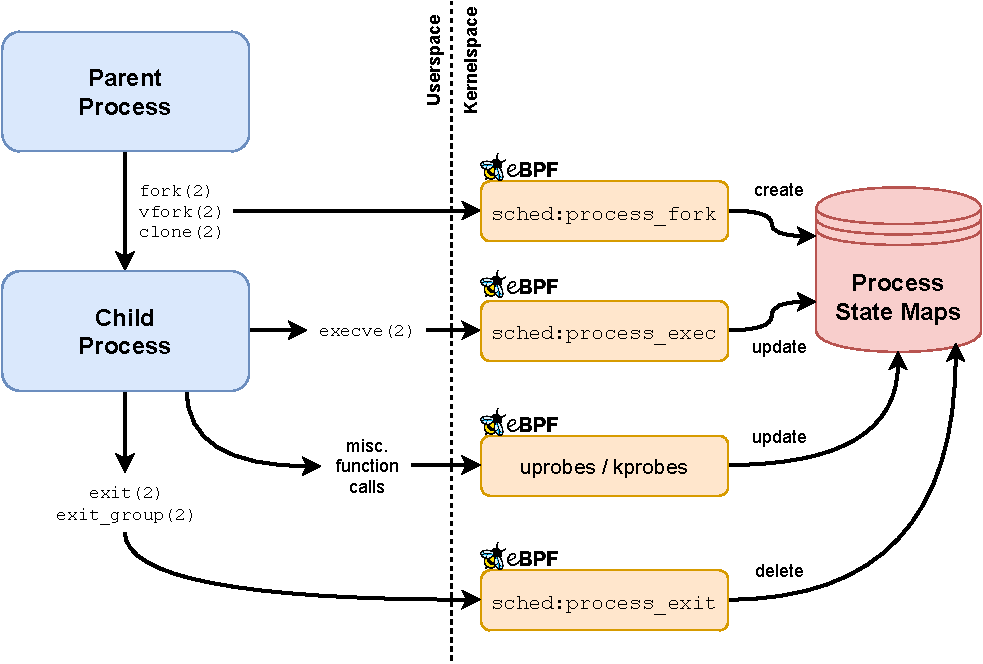
\includegraphics[width=0.8\linewidth]{figs/bpfbox/process-lifecycle.pdf}
  \caption[The various mechanisms that \bpfbox{} uses to manage process state]{
    The various mechanisms that \bpfbox{} uses to manage process state.
    Probes marked \texttt{sched:*} are tracepoints instrumenting scheduler events
    in the kernel. Uprobes and kprobes instrument userspace
    and kernelspace function calls respectively.
  }\label{fig:bpfbox-process-lifecycle}
\end{figure}



Instrumenting a tracepoint on \texttt{sched:process\_fork} allows \bpfbox{} to
detect when a new task is created via the \texttt{fork(2)}, \texttt{vfork(2)}, or
\texttt{clone(2)} system calls. This tracepoint creates an entry in the \textit{process
states} hashmap and initializes it according to the state of the parent process; if the
parent process is associated with a \bpfbox{} profile, its key is copied to the child
until such time as the child makes an \texttt{execve(2)} call.

The \texttt{sched:process\_exec} tracepoint is triggered whenever a task calls
\texttt{execve} to load a new program.  \bpfbox{} uses this tracepoint to manage the
association of \textit{policy keys} to a particular \textit{process state}.  \bpfbox{}
policy may optionally specify whether a transition from one profile to another may occur
in a given call to \texttt{execve}; this transition is disallowed by default.

Finally, the \texttt{sched:process\_exit} tracepoint allows \bpfbox{} to detect when
a task exits. This tracepoint deletes the corresponding entry in the \textit{process
states} map.

\subsection{Context-Aware Policy}
\label{ss:bpfbox-context-aware}

If the policy for a given executable defines specific function call contexts for
particular rules, \bpfbox{} instruments these function calls using uprobes (for userspace
functions) and kprobes (for kernelspace functions). Each instrumented function call is
associated with a unique bit in the process' \textit{state} bitmask.  A probe is triggered
on entry that causes \bpfbox{} to flip the corresponding bit to a \texttt{1}, and again on
return, flipping the corresponding bit back to a \texttt{0}.
\Cref{fig:bpfbox-function-calls} depicts how \bpfbox{} instruments userspace and
kernelspace function calls for policy enforcement.

\begin{figure}[p]
  \centering
  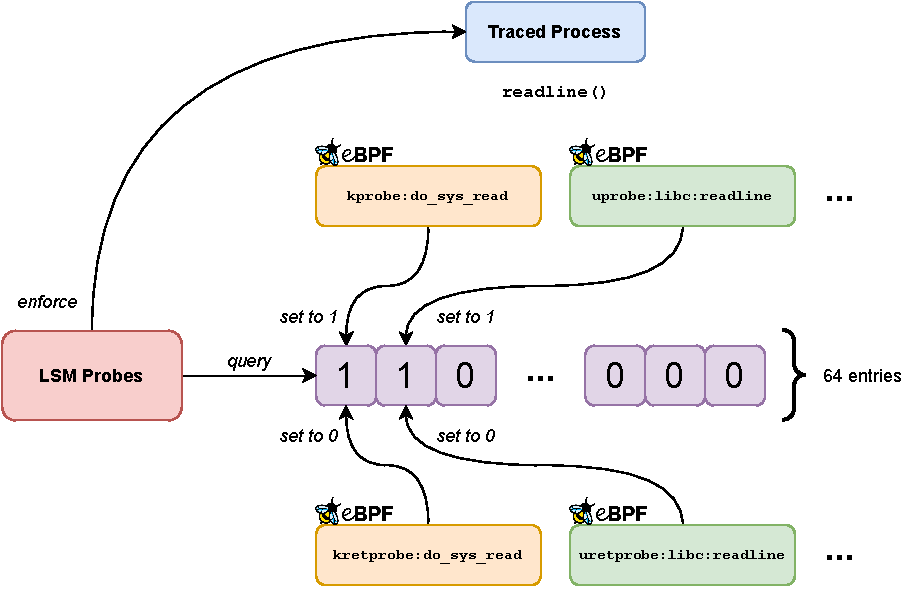
\includegraphics[width=1\linewidth]{figs/bpfbox/function-calls.pdf}
  \caption[How \bpfbox{} tracks function calls]{
    How \bpfbox{} uses kprobes and uprobes to track function calls.  If a policy
    identifies that a rule should apply within the context of a certain function call,
    \bpfbox{} instruments a probe on function entry and return. These probes flip the
    corresponding bit in the process' state vector, indicating to policy enforcement
    probes whether or not the process is in the middle of making the function call.
  }\label{fig:bpfbox-function-calls}
\end{figure}

This approach is subject to a few inherent limitations.  Firstly, compile-time
optimizations such as function inlining can invalidate the probe by removing the
corresponding symbol in the target object file. Secondly, a recursive call that is not
tail-optimized will break enforcement by prematurely signalling to \bpfbox{} that
a process has exited a given function context.  The first limitation may be trivially
worked around by hinting to the compiler that a given function should not be inlined;
although this sacrifices some application transparency and incurs a slight performance
penalty, the potential security benefits from such a fine-grained policy are arguably
worth the trade-off.  The second limitation \textit{could} be worked around by maintaining
a reference counter for each function call rather than a flat vector. \bpfbox{} currently
does not do this, since it would incur a larger memory overhead for each active process,
but it would be possible to extend a future version of \bpfbox{} with this workaround. In
case working around these limitations is impractical, the policy author would simply fall
back to specifying ordinary rules rather than context-specific ones.



\subsection{Collecting and Logging Audit Data}\label{ss:bpfbox-audit}

When an operation is denied or matches with an audit rule, \bpfbox{} submits an event to
userspace for logging. To accomplish this, we leverage the new ringbuf map type added in
Linux 5.8. The \gls{ebpf} ringbuf map implements an efficient ring buffer that is shared
across all \glspl{cpu}. This new map type comes with a number of optimizations for fast
reads and writes and in-order guarantees for asynchronous events across multiple
\glspl{cpu}, allowing per-event data to be efficiently shared with userspace in near
real time.

In userspace, the \bpfbox{} daemon uses \texttt{mmap(2)} to map the corresponding memory
region and polls for new data at regular intervals. As events are consumed in userspace
they are removed from the ring buffer to make room for new events.  Since the ringbuf map
provides strong order guarantees and high performance under contention, we can ensure that
\bpfbox{} always provides highly reliable and performant per-event auditing.



\section{\bpfbox{} Policy Language}\label{s:bpfbox-policies}

\bpfbox{} policies are a series of rules and accompanying decorators. A decorator may
annotate either individual rules or blocks of rules denoted by braces and is used to
specify additional context or policy actions. The first line in a \bpfbox{} policy is
always a special \enquote{profile decorator}, written as
\lstinline[language=bpfbox]{#![profile "/path/to/exe"]}, which marks the executable to
which the policy should be associated.  Other than the profile decorator, all others take
the form of \lstinline[language=bpfbox]|#[decorator] { rule() }|. Multiple decorators may
be specified before a set of rules, meaning that all decorators apply to each rule.

Profile assignment occurs when a process makes an \texttt{execve(2)} call that results in
loading the specified executable.  Once a process has been assigned a profile, this
profile cannot change again, unless an \texttt{execve(2)} occurs which has been explicitly
marked with the \lstinline[language=bpfbox]{#[transition]} decorator. This ensures that
policy transitions only occur when expected and prevents malicious \texttt{execve(2)}
calls from changing \bpfbox{}'s treatment of a process.

The sections that follow describe the rule categories supported by \bpfbox{}
(\Crefrange{ss:bpfbox-filesystem-rules}{ss:bpfbox-ptrace-rules}) and the decorators that
may optionally be used to augment them (\Crefrange{ss:bpfbox-allow}{ss:bpfbox-kfunc}).
\Cref{lst:bpfbox-policy-example} depicts a simple example \bpfbox{} policy.

\begin{lstlisting}[language=bpfbox, gobble=4,
  caption={[An example \bpfbox{} policy]
    An example \bpfbox{} policy for a simple remote login program. This example offers
    a fairly complete idea of the \bpfbox{} policy language's various features.
  },
  label={lst:bpfbox-policy-example}, float]
    /* This policy applies to the /usr/bin/mylogin
     * executable */
    #![profile "/usr/bin/mylogin"]

    /* Taint process state upon binding to
     * any IPv4/IPv6 network socket */
    #[taint] {
      net(inet,  bind)
      net(inet6, bind)
    }

    /* Allow network connections/operations */
    #[allow] {
      net(inet,  accept|listen|send|recv)
      net(inet6, accept|listen|send|recv)
    }

    /* Allow the check_login function to read
     * /etc/passwd and /etc/shadow */
    #[func "check_login"] {
      fs("/etc/passwd", read)
      fs("/etc/shadow", read)
    }

    /* Allow the add_user function to read
     * and append to /etc/passwd, but log such
     * events to the audit logs */
    #[func "add_user"]
    #[audit] {
      fs("/etc/passwd", read|append)
    }

    /* Read and append to any immediate child
     * of the /var/log/mylogin/ directory */
    fs("/var/log/mylogin/*", read|append)

    /* Allow the execution of /bin/bash, transitioning
     * profiles to bash's profile after the execve(2)
     * and untainting the process */
    #[transition]
    #[untaint] {
      fs("/bin/bash", read|exec)
    }
\end{lstlisting}



\subsection{Filesystem Rules}\label{ss:bpfbox-filesystem-rules}

Filesystem rules in \bpfbox{} govern what operations a process may perform on filesystem
objects such as files and directories. They are written as
\lstinline[language=bpfbox]{fs("pathname", access)} where
\lstinline[language=bpfbox]{"pathname"} is a string containing the pathname of the file
and \lstinline[language=bpfbox]{access} is a list of one or more file access permissions
joined by the vertical bar symbol.  For instance, to represent read and
append permissions on \texttt{/var/log/my\_log}, the corresponding \bpfbox{} rule would be
\lstinline[language=bpfbox]{fs("/var/log/my_log", read|append)}.  In total, \bpfbox{}
supports nine distinct filesystem access flags as shown in \Cref{tab:fs-access}.

\begin{table}[htpb]
    \centering
    \caption{The filesystem access flags supported in \bpfbox{}.}
    \label{tab:fs-access}
    \begin{tabular}{lp{0.7\linewidth}}
    \toprule
    Flag & Meaning \\
    \midrule
    \texttt{read}    & The subject may read the object. \\
    \texttt{write}   & The subject may write to the object. \\
    \texttt{append}  & The subject may append to the object. \\
    \texttt{exec}    & The subject may execute the object. \\
    \texttt{setattr} & The subject may change the object's filesystem attributes. \\
    \texttt{getattr} & The subject may read the object's filesystem attributes. \\
    \texttt{rm}      & The subject may remove the object's inode. \\
    \texttt{link}    & The subject may create a link to the object's inode. \\
    \texttt{ioctl}   & The subject may perform an ioctl call on the object. \\
    \bottomrule
    \end{tabular}
\end{table}

\bpfbox{} supports a limited globbing syntax when defining pathnames, allowing multiple
rules matching similar files to be combined into one.  Although filesystem rules are
specified using pathnames, \bpfbox{} internally uses inode and device numbers rather than
the pathnames themselves. When loading policies, \bpfbox{} automatically resolves the
provided pathnames into their respective inode-device number pairs. This information is
then used to look up the correct policy whenever a sandboxed application attempts to
access an inode.  Since \bpfbox{} does not check the pathnames themselves when referring
to files, it is able to defeat \glsentryfull{toctou} attacks, where an
attacker quickly swaps out one file with a link to another in an attempt to circumvent
access control restrictions in a privileged (most often setuid)
binary~\cite{bishop1996_checking}.  In such a situation, \bpfbox{} would simply see
a different inode and deny access.

In addition to regular filesystem rules, \bpfbox{} provides a special rule type for
\texttt{/proc/pid} entries in the \texttt{procfs} virtual filesystem. \texttt{procfs}
rules, written as \lstinline[language=bpfbox]{proc("exe", access)} where
\lstinline[language=bpfbox]{"exe"} is a string containing the pathname of another
executable and \lstinline[language=bpfbox]{access} is the desired access. For example,
read-only access to the \texttt{procfs} entries of executables running
\texttt{/usr/bin/ls} may be specified with \lstinline[language=bpfbox]{proc("/usr/bin/ls", read)}.
Access to any \texttt{procfs} entry may be specified using the special keyword
\lstinline[language=bpfbox]{any}.



\subsection{Network Rules}\label{ss:bpfbox-network-rules}

\bpfbox{} implements networking policy at the socket level, covering both Internet sockets
as well as Unix domain sockets. Networking rules are specified using
\lstinline[language=bpfbox]{net(protocol, access)}, where
\lstinline[language=bpfbox]{protocol} is a networking protocol like \texttt{inet},
\texttt{inet6}, or \texttt{unix} and \lstinline[language=bpfbox]{access} is a list of
socket operations (\Cref{tab:net-access}) separated by vertical bars. For example, a rule
targeting \texttt{bind}, \texttt{accept}, and \texttt{connect} operations on an
\texttt{inet6} socket would look like \lstinline[language=bpfbox]{net(inet6, bind|connect|accept)},
while a rule targeting \texttt{create} operations on a \texttt{unix} socket would look
like \lstinline[language=bpfbox]{net(unix, create)}.

\begin{table}[htpb]
    \centering
    \caption{The socket operation flags supported in \bpfbox{}.}
    \label{tab:net-access}
    \begin{tabular}{lp{0.7\linewidth}}
    \toprule
    Flag & Meaning \\
    \midrule
    \texttt{connect}  & Subject may connect a socket to a remote address. \\
    \texttt{bind}     & Subject may bind a socket to a local address. \\
    \texttt{accept}   & Subject may accept an incoming socket connection. \\
    \texttt{listen}   & Subject may listen for incoming socket connections. \\
    \texttt{send}     & Subject may send messages over a socket. \\
    \texttt{recv}     & Subject may receive messages over a socket. \\
    \texttt{create}   & Subject may create new sockets. \\
    \texttt{shutdown} & Subject may shut down a socket connection. \\
    \bottomrule
    \end{tabular}
\end{table}



\subsection{Signal Rules}\label{ss:bpfbox-signal-rules}

Specifying signal behaviour in \bpfbox{} is done using the
\lstinline[language=bpfbox]{signal("exe", access)} where
\lstinline[language=bpfbox]{"exe"} is the pathname of another executable and
\lstinline[language=bpfbox]{access} is a list of signals allowed to be sent, separated by
vertical bars. Normally, only processes running the executable
\lstinline[language=bpfbox]{"exe"} are allowed to be signalled, but the special keyword
\lstinline[language=bpfbox]{any} may be used instead to specify the ability to signal
\textit{any} process on the system. Two additional keywords,
\lstinline[language=bpfbox]{parent} and \lstinline[language=bpfbox]{child}, allow parent
and child processes to be signalled instead.  The \lstinline[language=bpfbox]{access}
argument supports any Linux signal, in addition to a few helper keywords that can be used
to specify broad categories, such as \lstinline[language=bpfbox]{fatal} for fatal signals
and \lstinline[language=bpfbox]{nohandle} for signals that cannot be handled.  For
example, to specify the ability to send fatal signals to any process running
\texttt{/usr/bin/ls}, the corresponding \bpfbox{} rule would be
\lstinline[language=bpfbox]{signal("/usr/bin/ls", fatal)}.  To narrow permissions such
that only \texttt{SIGTERM} and \texttt{SIGINT} are allowed,
\lstinline[language=bpfbox]{signal("/usr/bin/ls", sigterm|sigint)} could be used instead.



\subsection{Ptrace Rules}\label{ss:bpfbox-ptrace-rules}

Just like with signals, \texttt{ptrace} access is specified as
\lstinline[language=bpfbox]{ptrace("exe", access)}, where
\lstinline[language=bpfbox]{access} is a list of allowed \texttt{ptrace} modes separated
by vertical bars. The \lstinline[language=bpfbox]{child} keyword is also available for
\texttt{ptrace} rules to allow tracing of any child process, regardless of the child's
current profile. For instance, a rule that allows a process to read and attach to a child
process would be written as \lstinline[language=bpfbox]{ptrace(child, read|attach)}, while
a rule that allows only read access to processes running \texttt{/usr/bin/ls} would be
written as \lstinline[language=bpfbox]{ptrace("/usr/bin/ls", read)}.  Note that currently
\texttt{ptrace} rules do not override other \texttt{ptrace} restrictions, such as those
imposed by Yama~\cite{yama}.



\subsection{Allow, Taint, and Audit Decorators}\label{ss:bpfbox-allow}

\bpfbox{} supports three distinct decorators for defining \textit{actions} that should be
taken when a given access matches a rule. The \lstinline[language=bpfbox]{#[allow]}
decorator causes \bpfbox{} to allow the access; however, it is not typically necessary to
explicitly specify this as undecorated rules are assumed to be allowed by default.
Regardless, it may be desirable to decorate such rules with
\lstinline[language=bpfbox]{#[allow]} to improve the clarity of the policy.
\lstinline[language=bpfbox]{#[taint]} is used to mark a rule as a \textit{taint rule},
which causes the process to enter a tainted state when matched. These rules can be thought
of as gateways into the rest of the policy.  Once a process is tainted, this cannot be
reversed unless it makes an \texttt{execve(2)} call explicitly marked with
\lstinline[language=bpfbox]{#[untaint]}.  Finally, \lstinline[language=bpfbox]{#[audit]}
may be combined with \lstinline[language=bpfbox]{#[allow]} to cause \bpfbox{} to log the
matching operation to its audit logs. This can be useful for marking rare behaviour that
should be investigated or for determining how often a given rule is matched in practice.



\subsection{Func and Kfunc Decorators}\label{ss:bpfbox-kfunc}

One of the key features of \bpfbox{} is the ability to specify specific application-level
and kernel-level context for rules. In the policy language, this is done by decorating
rules with the \lstinline[language=bpfbox]{#[func "fn_name" ("filename")]} and
\lstinline[language=bpfbox]{#[kfunc "fn_name"]} decorators for userspace and kernelspace
instrumentation respectively. Here, \lstinline[language=bpfbox]{"fn_name"} refers to the
name of the function to be instrumented and \lstinline[language=bpfbox]{"filename"} refers
to the filename where the function symbol should be looked up --- this parameter is
optional and allows for the instrumentation of shared libraries.  These decorators provide
powerful tools for defining extremely fine-grained, sub-application level policy. For
instance, to declare that read access to the file \texttt{/etc/shadow} should only occur
during a call to the function \texttt{check\_password()}, the corresponding \bpfbox{} rule
would look like:
\begin{lstlisting}[language=bpfbox]
#[func "check_password"]
fs("/etc/shadow", read)
\end{lstlisting}
A process that is sandboxed using this policy would be unable to access
\texttt{/etc/shadow} except within a call to the specified function.



\section{State of the \bpfbox{} Implementation}
\label{s:bpfbox-discrepancies}

This chapter has presented \bpfbox{} as it was originally designed. However, some aspects
of the \bpfbox{} policy language were never fully realized, despite being implemented on
the \gls{ebpf} side. In particular, decorators to transition profiles and untaint
a process when making an execve call are currently unimplemented. Other aspects of the
policy language, such as the formulation of ptrace rules, also differ from the current
implementation. Before a full implementation could be completed, the transition toward
\bpfcontain{} (c.f.\ \Cref{c:bpfcontain}) had already begun; in our view, \bpfcontain{} is
a successor to \bpfbox{}, and thus deprecates the original \bpfbox{} implementation. As
a result, many of the unimplemented aspects of \bpfbox{}'s policy language are reflected
in the \bpfcontain{} implementation, either through its policy language schema
(\Cref{s:bpfcontain-policy}), or through its default policy enforcement
(\Cref{ss:bpfcontain-default}).



\section{Summary}\label{s:bpfbox-summary}

This chapter has presented the design and implementation of \bpfbox{}, a prototype process
confinement mechanism leveraging \gls{ebpf} for dynamically loadable policies that balance
simplicity and flexibility. In particular, we outline \bpfbox{}'s architecture, the
implementation details of its \gls{ebpf}-based policy enforcement mechanism, and the
design of its custom policy language. Through a combination of \gls{ebpf}-based
enforcement and a lightweight yet fine-grained policy language, \bpfbox{} represents
a step towards the container-specific design outlined in \Cref{s:cp-design}.  In the next
chapter, we outline \bpfcontain{}, an iteration of \bpfbox{} that addresses a few of its
fundamental limitations and makes a transition toward container-specific policies.


\chapter{\bpfcontain: Extending \bpfbox{} to Model Containers}\label{c:bpfcontain}
In this chapter, we present \bpfcontain{}, an iteration on the original \bpfbox{} system
presented in \Cref{c:bpfbox}. \bpfcontain{} is a superset of \bpfbox. In particular, it is
a streamlined re-implementation that focuses on container-specific confinement policy, low
dependency overhead, and maximizing adoptability. Portions of this chapter are taken from
an upcoming paper, co-authored with David Barrera and Anil Somayaji, and planned for
submission at USENIX Security 2022. A draft of this paper is currently
available~\cite{findlay2021_bpfcontain}, although significant portions of this chapter
differ from the publicly available archive due to subsequent updates to \bpfcontain{}.



\section{\bpfbox{}'s Limitations and the Transition Toward \bpfcontain{}}\label{s:bpfcontain-bpfbox-limitations}

The previous chapter presented \bpfbox{}, a prototype process confinement mechanism and
precursor to \bpfcontain{}. While \bpfbox{} certainly offers a new perspective on
confinement and improves the status quo, the extent to which it achieves the design goals
outlined in \Cref{s:cp-design} of \Cref{c:confinement-problem} is arguably hampered by
a few inherent limitations. We enumerate and describe these limitations as follows.  The
goal is to examine these limitations as an early motivating factor for the development of
\bpfcontain{}, which will inform later comparisons between these two systems
(c.f.\ \Cref{s:bpfcontain-improvements}).

\begin{enumerate}
  \item \textbf{Dependency Overhead and Runtime Overhead.}
    Due to its userspace implementation using bcc, \bpfbox{} has a high dependency
    overhead. This overhead is the combined result of a number of requirements imposed on
    the host system by the bcc toolchain. On the userspace side, bcc depends on Python as
    well as the entire LLVM toolchain for program compilation. Both of these are rather
    hefty requirements on their own. Python requires an entire language runtime, and
    a full LLVM toolchain can introduce hundreds of megabytes of additional code
    (approximately 587MiB when installing LLVM version 12.0 on Arch Linux).

    Furthermore, Python and bcc incur significant runtime overhead. Python is an
    interpreted language with a much heavier runtime than compiled systems languages like
    C or Rust.  This runtime incurs additional performance disadvantages due to safety
    features like the global object lock, which impede concurrency. Since bcc compiles
    \gls{ebpf} programs at runtime, we incur additional compilation overhead for each
    program, sometimes resulting in significant startup delays depending on the complexity
    of the application. The runtime compilation of \gls{ebpf} programs also necessitates
    the availability of kernel headers as a compilation dependency in the target
    environment, adding further storage overhead (approximately 129MiB for Linux
    5.12 on a stock Arch kernel).

  \item \textbf{Lack of Container Semantics.}
    Although \bpfbox{} exposes a lightweight policy language with high-level semantics to
    the user, it fails to consider container semantics, as outlined in design goal
    \ref{i:dg-suitability} in \Cref{s:cp-design}. While this marks an improvement over
    existing confinement solutions by offering a terse yet expressive policy language, it
    fails to fully address the container-specific use case; in other words, \bpfbox{} is
    more suitable to generic, ad-hoc application sandboxing than to container-specific
    applications. In improving how the \bpfbox{} model handles containers, we can
    simultaneously simplify policies and improve security by defining a clear protection
    boundary around a container.

  \item \textbf{Policy Language Improvements.}
    In addition to adding container semantics, other aspects of the \bpfbox{} policy
    language can also be improved and simplified. For instance, \bpfbox{} implements
    policy in a domain-specific policy language, designed specifically with \bpfbox{}'s
    enforcement engine in mind. While effective, this approach is tightly-coupled with
    policy enforcement and introduces additional cognitive overhead when making extensions
    to or modifying the policy language design. Furthermore, learning the syntax of
    a custom policy language can introduce an additional barrier-to-entry for new policy
    authors, to the detriment of \bpfbox{}'s original goal of making policy authorship
    available to end users.
\end{enumerate}

\subsection{Motivating \bpfcontain{}}

The key insight behind \bpfcontain{} is that \bpfbox{} approached the confinement problem
(c.f.\ \Cref{c:confinement-problem}) from a \textit{per-process} perspective. When dealing
with containers, we should instead approach the confinement problem from
a \textit{per-process-group} perspective. That is, we expand the unit of confinement from
an individual process to a collection of related processes. Specifically, our goal is to
define a clear boundary between the container and the outside world, while minimizing the
friction between two subjects that operate within this boundary.

Under \bpfbox{}, policies applied to individual applications, inheriting policy across
forks, and selectively transitioning across execves. While this model is effective for
application-level confinement, it fails to meet the needs of a container-specific
deployment.  Conversely, \bpfcontain{} expands this model to incorporate container
semantics, grouping processes into a container and enforcing a protection boundary around
the container.  Implementing confinement in this way requires some fundamental changes to
both the underlying policy language and policy enforcement mechanism. In particular, we
alter the policy language to work with higher level semantics that support container-level
confinement. Moreover, \bpfcontain{}'s enforcement engine employs a more nuanced default
policy that considers the relationship between processes and resources that exist within
the context of a container. These changes from a policy and enforcement perspective enable
\bpfcontain{} to enforce simple container-level policies while reusing the initial ideas
from \bpfbox{}: namely, dynamic, lightweight enforcement based on \gls{ebpf}.

While implementing \bpfcontain{}, opportunities arose to improve how it handles
dependencies and manages the lifecycle of its \gls{bpf} programs and maps. Specifically,
we architect \bpfcontain{} based on Rust, libbpf-rs~\cite{libbpf-rs}, and \gls{bpf}
\gls{core}~\cite{nakryiko2020_core}. These changes totally eliminate the runtime overhead
introduced by \gls{bpf} program compilation and the dependency overhead from LLVM and
kernel headers. Further, \gls{core} enables \bpfcontain{} to work seamlessly across
multiple kernel versions and configurations. These changes improve the adoptability of
\bpfcontain{}, particularly in containerized environments, wherein heavyweight
dependencies can critically impact deployments.

\Cref{tab:bpfcontain-comparison} offers a high-level comparison between the properties and
features of \bpfbox{} and \bpfcontain{}. This comparison provides a high-level overview of
the major differences and motivating properties in each design. The sections that follow
will discuss each of these items in detail.

\begingroup\small
\begin{longtable}[c]{r||ll}
\caption[Comparing \bpfbox{} and \bpfcontain{}]{
    Comparing \bpfbox{} and \bpfcontain{} by their properties and how well each satisfies
    the design goals outlined in \Cref{s:cp-design}.
}\label{tab:bpfcontain-comparison}\\
  \toprule
  Property/Goal              & \bpfbox{}        & \bpfcontain{} \\
  \midrule
  Userspace Implementation   & Python + bcc     & Rust + libbpf-rs\\
  Kernelspace Implementation & bcc + LLVM       & \glsentryshort{bpf} \glsentryshort{core} \\
  Dependencies               & $>800\text{MiB}$ & $<5\text{MiB}$ \\
  State Management           & Process-Level    & Container-Level    \\
  Default Policy             & Default-Deny     & Container Boundary\textsuperscript{\textdagger} \\
  Policy Language            & Custom DSL       & YAML/JSON/TOML \\
  \midrule
  Simple/Flexible Policies?  & Yes              & Yes \\
  Suitable for Containers?   & No               & Yes \\
  High Adoptability?         & Somewhat\textsuperscript{\textdaggerdbl}         & Yes \\
  \bottomrule
  \multicolumn{3}{p{4.5in}}{\footnotesize \textsuperscript{\textdagger}\bpfcontain{}'s policy
  defaults are more nuanced than \bpfbox{}. We enforce a default-allow policy on resources
  \textit{within} the container, and a default-deny policy on resources \textit{outside}
  of the container. See \Cref{ss:bpfcontain-default} for details.}\\
  \multicolumn{3}{p{4.5in}}{\footnotesize \textsuperscript{\textdaggerdbl}While \bpfbox{} has
  a more adoptability than an out-of-tree \gls{lsm} (due to \gls{ebpf}), its practical
  adoption is hampered by heavy runtime dependencies and incompatibility with the
  container model.}
\end{longtable}
\endgroup

\section{\bpfcontain{} Overview}\label{s:bpfcontain-overview}

\bpfcontain{} is a container security daemon for Linux with an emphasis on simple,
high-level confinement policies for container deployments. Although it is expressly
designed to work with container semantics in mind, \bpfcontain{} implements a superset of
\bpfbox{}'s capabilities (c.f.\ \Cref{c:bpfbox}) and works for confining ordinary
applications as well as containers. To achieve confinement, \bpfcontain{} leverages
\gls{ebpf} programs attached to \gls{lsm} hooks in the kernel for security enforcement.

As a container-specific confinement solution, \bpfcontain{} has a number of important
design goals, some of which are shared with \bpfbox{}. First, we seek to design a simple
yet flexible policy language that supports ad-hoc confinement use cases, enabling an
end user to write a custom confinement policy to suit their needs. We extend this goal by
seeking to make the policy language and enforcement engine \textit{container specific}.
This means that \bpfcontain{} policies should conform to container semantics and work in
tandem with container virtualization primitives to improve policy enforcement and further
simplify the underlying policies. An implicit sub-goal of container-specific policy is to
improve the level of confinement afforded to container deployments, bringing security more
in line with that of alternative isolation techniques, such as virtual machines. Finally,
\bpfcontain{} should be readily adoptable in production use cases and should be useful for
confining existing container workloads.

At the surface level, \bpfcontain{}'s architecture is similar to that of \bpfbox{}, albeit
with significant differences in implementation and design details. In a nutshell,
\bpfcontain{} is implemented as a privileged userspace daemon that loads \gls{ebpf}
programs and maps into the kernel, which then enforce policy.
\Cref{ss:bpfcontain-enforcement-overview} provides a high-level overview of how
\bpfcontain{} enforces policy, whereas \Cref{s:bpfcontain-implementation} covers
\bpfcontain{}'s architecture and implementation details in full.

\subsection{Policy Enforcement at a High Level}\label{ss:bpfcontain-enforcement-overview}

\bpfcontain{} enforces confinement policy using \gls{ebpf} programs attached to \gls{lsm}
hooks in the kernel. Like \bpfbox{}, \bpfcontain{} leverages the
\gls{krsi}~\cite{singh2019_krsi} \gls{lsm} programs introduced in Linux 5.7 for this
purpose. Unlike \bpfbox{}, \bpfcontain{} generates \gls{bpf} bytecode at
\textit{compile time} rather than at runtime. The bytecode is then embedded directly in
\bpfcontain{}'s binary object file, where it can subsequently be loaded into the kernel at
runtime. This has the benefit of eliminating initial compile-time overhead and supporting
cross-architecture deployments using \gls{bpf} \gls{core}.

To confine a container, an administrator authors a high-level confinement policy that
specifies which operating system interfaces and resources should be exposed to the
container.  Thanks to a modular approach to encoding and decoding policies, \bpfcontain{}
policies may be written in a number of user-facing data serialization languages, including
YAML~\cite{yaml}, TOML~\cite{toml}, and JSON~\cite{json}. (For the rest of this thesis, we
assume the YAML format for simplicity.) At a minimum, \bpfcontain{} policies include
a policy name, along with a few tunable parameters. From there, the administrator may
specify zero or more policy rules over three distinct categories: allow, deny, and taint.
We cover \bpfcontain{} policy in more detail in \Cref{s:bpfcontain-policy}.

\begin{figure}[htpb]
  \centering
  \includegraphics[width=1\linewidth]{figs/bpfcontain/overview.pdf}
  \caption[A high-level overview of how \bpfcontain{} confines containers]{
    A high-level overview of how \bpfcontain{} confines containers.  At compile-time,
    the object code for \bpfcontain{}'s \gls{bpf} programs is embedded directly into the
    resulting binary. To confine a container, the user first authors a high-level policy
    in their chosen data serialization language. The daemon parses this policy and loads
    it into the kernel by encoding it into \gls{ebpf} maps. The user then launches the
    container using the \texttt{bpfcontain-run} wrapper, at which point \bpfcontain{}
    begins tracing it and enforcing policy. Note the subtle differences between this
    figure and \Cref{fig:bpfbox-policy-overview} in \Cref{c:bpfbox}.
  }\label{fig:bpfcontain-overview}
\end{figure}

The \bpfcontain{} daemon runs as a privileged process, parsing and loading user policy by
encoding it into a series of \gls{bpf} maps. The user then launches their container using
an unprivileged wrapper program, \texttt{bpfcontain-run}. The sole task of this wrapper
application is to invoke a stub function which does nothing more than pass the desired
policy ID as an argument. \bpfcontain{} traces this function call and uses it to confine
the container with the correct policy. Unlike \bpfbox{}, this technique enables the user
to associate any container with any policy, rather than a fixed one-to-one mapping.

At runtime, \bpfcontain{}'s \gls{bpf} programs trace the behaviour of processes running
under the container and confine it according to a mixture of default policy and policy
rules specified by the user. Like \bpfbox{}, enforcement is accomplished primarily through
\gls{bpf} programs attached to \gls{lsm} hooks in the kernel. The precise implementation
details of these programs vary significantly, and are covered in detail in
\Cref{s:bpfcontain-implementation}. \Cref{fig:bpfcontain-overview} illustrates
a high-level overview of the policy enforcement process described here.



\section{\bpfcontain{} Implementation}\label{s:bpfcontain-implementation}

This section presents the implementation details and architecture of \bpfcontain{}'s
policy enforcement mechanism. Specifically, we provide an initial overview of
\bpfcontain{}'s userspace and kernelspace components, then examine how \bpfcontain{}
enforces policy in the kernel using \gls{ebpf}. Whereas this section focuses specifically
on policy enforcement, \Cref{s:bpfcontain-policy} outlines and documents the details of
\bpfcontain{}'s policy language.

\subsection{Architectural Overview}\label{ss:bpfcontain-architecture}

Like \bpfbox{}, \bpfcontain{} is implemented as privileged daemon that runs in userspace
and loads \gls{ebpf} code into the kernel for policy enforcement. However, the precise
architecture and implementation details of this daemon are quite different. In particular,
the daemon is implemented in Rust and leverages the libbpf-rs crate\footnote{A crate is
a Rust package that can be added as a dependency to a project. For the purposes of this
thesis, we can consider the terms \enquote{crate} and \enquote{library} to be
equivalent.}~\cite{libbpf-rs} to load its \gls{ebpf} programs and maps into the kernel.
This results in a number of advantages, which we discuss in more detail in the following
section.

\bpfcontain{}'s kernelspace \gls{ebpf} programs trace container lifecycle and enforce
policy, while \gls{ebpf} maps store policy and pass intermediary state between program
invocations. This architecture is similar in spirit to the design of \bpfbox{}, but with
a few fundamental differences. Rather than using the LLVM toolchain to compile
programs at runtime, \bpfcontain{} pre-compiles and embeds the \gls{bpf} object code into
its binary object file. Using \gls{bpf} \gls{core}~\cite{nakryiko2020_core}, these
programs can then be dynamically loaded into any supported kernel, regardless of the
underlying configuration or architectural details.

\bpfcontain{} leverages several \gls{bpf} program and map types to implement container
tracing and confinement. While many of the major program types are shared with \bpfbox{},
there are a few distinct differences (c.f.\ \Cref{ss:bpfbox-architecture}). We enumerate
these differences as follows. Map types are outlined in \textbf{\green{green}} and program
types are outlined in \textbf{\purple{purple}}.

\paragraph*{Maps:}
\begin{itemize}
  \item \bpfcontain{} replaces many of \bpfbox{}'s \textbf{\green{Hash Maps}},
  particularly those used to track process state, with equivalent \textbf{\green{Local
  Storage Maps}}. Local storage is a new \gls{ebpf} map type supported in the latest
  kernels (Linux 5.11 and onwards). Local storage maps tether the underlying value to
  a kernel data structure, such as a task or inode, used as a key into the map. The result
  is a dynamically-allocated and garbage-collected per-structure storage blob.
  \bpfcontain{} leverages these for more memory-efficient storage of per-task and
  per-inode state.
\end{itemize}

\paragraph*{Programs:}
\begin{itemize}
  \item \bpfcontain{} replaces the use of scheduler \textbf{\purple{Tracepoints}} with
  equivalent \textbf{\purple{\gls{lsm} Probes}} that expose the same information. This
  reduces potential overhead from multiple \gls{bpf} program invocations on the same code
  path, most notably over \texttt{fork(2)} and \texttt{clone(2)} family system calls.

  \item \bpfcontain{} uses \textbf{\purple{Fentry and Fexit}} probes in place of
  \textbf{\purple{Kprobes}}. These use a more efficient trampoline technique for program
  entry and use \gls{btf} information exposed by the kernel for direct memory access,
  making them far more efficient than kprobes\footnote{However, the majority of \bpfbox{} and
  \bpfcontain{}'s \gls{ebpf} programs are \gls{lsm} probes rather than kprobes or fentry
  probes. As a result, this design change has little consequence on overall performance overhead.}.
\end{itemize}

Aside from the aforementioned differences, \bpfcontain{} uses the same \gls{bpf} program
and map types as \bpfbox{}. However, the underlying implementation details of each
\gls{bpf} program will be quite different from \bpfbox{}, as \bpfcontain{} is dealing with
container semantics, new policy rules, and more nuanced policy defaults. We examine the
most important implementation details in the subsections that follow.



\subsection{Policy Deserialization and Loading}\label{ss:bpfcontain-serde}

When designing the \bpfcontain{} policy language, we made a conscious design decision to
avoid constraining the user to one specific language syntax. In particular, we wanted to
avoid another domain-specific language, as learning the policy language could be a barrier
to entry for new users. A domain-specific policy language also presents issues when making
changes to or adding new features to the policy language specification, as the parser and
lexer must both be modified, along with underlying rule representation and enforcement
engine. Instead, we elected to decouple the policy language from the policy specification,
using Serde~\cite{serde}, a data serialization and deserialization crate for Rust.

Serde leverages Rust's powerful type system and procedural macros to derive serialization
and deserialization logic for vanilla Rust structs and enums. Rust crates that consume
Serde's \gls{api} can then use the automatically generated logic for serialization and
deserialization. This design enables a plug-and-play relationship between a data schema,
defined as a Rust data structure, and any data serialization language supported through the
Rust crates ecosystem. \bpfcontain{} uses Serde to automatically generate the accompanying
deserialization logic for a \texttt{Policy} struct and several \texttt{Rule} structs, one
for each supported rule type. \Cref{lst:bpfcontain-serde} depicts a simplified example of
how this works.

\begin{lstlisting}[language=Rust, gobble=2, caption={[A simplified example of \bpfcontain{}'s policy deserialization logic]
  A simplified example of \bpfcontain{}'s policy deserialization logic. Policy rules are
  specified declaratively using Rust structs and the corresponding deserialization logic
  is automatically generated by the Serde crate using a simple decorator macro.
},
label={lst:bpfcontain-serde}]
  use serde::Deserialize;

  /// The policy data structure
  #[derive(Deserialize)]
  pub struct Policy {
    name: String,
    /* Other policy metadata would go here... */
    allow: Vec<Rule>,
    deny: Vec<Rule>,
    taint: Vec<Rule>,
  }

  /// An enum encompassing all rule types
  #[derive(Deserialize)]
  pub enum Rule {
    FileRule(FileRule),
    /* Other rule types would go here... */
  }

  /// A "file access" rule
  #[derive(Deserialize)]
  pub struct FileRule {
    pathname: String,
    access: String,
  }

  /* Other rule types would go here... */
\end{lstlisting}

To enable the daemon to encode policy as an \gls{ebpf} map, each rule type implements the
\texttt{LoadableRule} trait. The daemon uses this logic to convert a policy rule into
a canonical format that can be represented in the kernel and thus used to enforce security
policy. Implementing this trait is as simple as writing a \texttt{load()} function that
makes a series of map updates to load the rule into the kernel; we leverage
libbpf-rs~\cite{libbpf-rs} for this purpose. When loading a policy into the kernel, the
daemon simply invokes this \texttt{load()} function for each policy rule.

Implementing policy deserialization and loading logic in this way has a number of
advantages. Since the policy schema is simply encoded declaratively in vanilla Rust, it is
easy for a developer (even a new contributor to \bpfcontain{}) to implement a new rule
type and add it to \bpfcontain{}. Adding a new rule type is as simple as defining a new
Rust data type to represent the rule and implementing the \texttt{LoadableRule} trait,
enabling the daemon to encode the rule as an \gls{ebpf} map. Due to Serde's modular
design, supporting a new serialization language for \bpfcontain{} policies is trivial; we
simply pull in the corresponding consuming crate as a dependency. Currently, \bpfcontain{}
supports YAML, JSON, and TOML as policy language encodings, but this can easily be
extended in future versions.

While these conveniences may add some modest performance overhead, this overhead is
incurred at policy load time and has no impact on any of \bpfcontain{}'s kernelspace code
paths. Therefore, we expect the overall impact of this design choice on system
performance to be minimal.

\subsection{Policy Enforcement}\label{ss:bpfcontain-enforcement}

Policy enforcement under \bpfcontain{} can be thought of as a combination of
\textit{explicit policy} (the rules defined in the policy file) and a nuanced
\textit{default policy} (the set of sensible defaults that \bpfcontain{} enforces to
define a boundary around the container). In particular, default access to resources is
determined based on whether that resource exists within the context of a container.
Resources within the container, such as \gls{ipc} handles into container processes or
filesystems belonging to the container's user namespace mount are considered
default allow. Conversely, resources outside of the container, such as external files or
processes, are considered default deny. Similarly, access is also denied to any operating
system interfaces that could affect global system state, such as character devices, kernel
modules, \gls{ebpf}, and some special filesystems. Exceptions to these defaults may
be explicitly defined in the policy file as required. \Cref{ss:bpfcontain-default}
examines the implementation of \bpfcontain{}'s default policy in more detail.

Like \bpfbox{}, \bpfcontain{} maintains its policy files in a root-controlled directory
(\texttt{/var/lib/bpfcontain/policy} by default). These policy files may be written in any
policy language supported by \bpfcontain{}'s policy deserializer, as documented in
\Cref{ss:bpfcontain-serde}. The \bpfcontain{} daemon watches the policy directory for
updates to policy files and triggers a reload of the corresponding policy when a file
changes. To load a policy, the daemon deserializes the policy file into a Rust data
structure consisting of a series of policy rules and accompanying metadata. It then
encodes this policy structure into a series of resource IDs and access vectors and loads
these into the correct policy maps in the kernel using the \texttt{bpf(2)} system call.
Once a policy has been loaded into the kernel, \bpfcontain{}'s \gls{ebpf} programs can
begin enforcing it.

To start confinement, a user invokes an unprivileged application, \texttt{bpfcontain-run},
which wraps the target executable. This wrapper's only purpose is to enable
\bpfcontain{}'s \gls{ebpf} programs to associate its process group with the correct policy
in the kernel.  This is done by invoking a stub function, traced by a \gls{usdt} probe.
When the probe fires, it reads the policy ID, passed as an argument to the stub, along
with other information such as the task's \gls{pid} and namespace membership taken from
its task struct in the kernel. The probe then updates a global process state map with this
information. Subsequent \gls{ebpf} programs use this information when making enforcement
decisions and when managing the container's state. \Cref{ss:bpfcontain-state} describes
state management in more detail.

\bpfcontain{} enforces most policy rules using \gls{krsi}~\cite{singh2019_krsi}, which
enables it to attach \gls{ebpf} programs to \gls{lsm} hooks in the kernel. In cases where
\gls{lsm} hooks alone are insufficient or no \gls{lsm} hook is exposed to guard the target
operation, \bpfcontain{} falls back to an fentry probe, hooking the underlying kernel
functions directly. In total, \bpfcontain{} instruments 46 \gls{lsm} probes, covering
filesystem, network socket, \gls{ipc}, and capability-level access, in addition to
miscellaneous privileged operations like loading a kernel module or updating an \gls{ebpf}
program or map. One fentry probe is used to prevent a container from modifying its
namespace membership after starting confinement.

\bpfcontain{} supports four distinct policy decisions for security-sensitive operations:
\texttt{allow}, \texttt{deny}, \texttt{taint}, or \texttt{forcequit}. A decision of
\texttt{allow} causes the access to be allowed, as normal. A decision of \texttt{deny}
results in the access being denied, and the corresponding system call returning
\texttt{-EACCES} to the user. A decision of \texttt{taint} causes \bpfcontain{} to taint
the container, a process that is similar in spirit to tainting under \bpfbox{}
(c.f.\ \Cref{ss:bpfbox-enforcement} of \Cref{c:bpfbox}). When a container is tainted, it
transitions into a stricter default-deny policy. Finally, a decision of \texttt{forcequit}
causes the kernel to terminate the offending process by delivering an uncatchable
\texttt{SIGKILL}\footnote{\texttt{SIGKILL} is a POSIX signal that causes a process to
immediately force quit. Unlike most signals, this signal cannot be ignored or handled by
the process.}. This decision is reserved for aggressive violations of \bpfcontain{}'s
default policy, such as a process attempting to load code into the kernel
(c.f.\ \Cref{ss:bpfcontain-default}).

When enforcing policy, \bpfcontain{} employs a simple heuristic to judge what the
resulting policy decision should be. If any rule matches a \texttt{deny} decision, the
operation is denied. If any rule matches a \texttt{taint} decision, the container is
tainted.  Finally, if no rule matches a \texttt{deny} decision and any rule matches an
\texttt{allow} decision, the operation is allowed. In the case where no rule matches are
found, \bpfcontain{} falls through to its default policy (\Cref{ss:bpfcontain-default}).
This process is depicted in full in \Cref{fig:bpfcontain-enforcement} on page
\pageref{fig:bpfcontain-enforcement}.

\subsection{Default Policy}\label{ss:bpfcontain-default}

Since \bpfcontain{} is designed to confine containers, it is able to achieve some nuanced
policy defaults by leveraging container-level semantics. This marks a significant
improvement over both conventional \glspl{lsm} such as SELinux and AppArmor, and the
original \bpfbox{} system, which each require the user to either explicitly mark each
desired access or to over-generalize access in favour of simpler policies. By taking
container semantics into account, \bpfcontain{} policies can be simultaneously expressive
and secure yet offer a simple path to achieving strong protection defaults.
\Cref{fig:bpfcontain-enforcement} depicts \bpfcontain{}'s default enforcement strategy.

\begin{figure}[p]
  \centering
  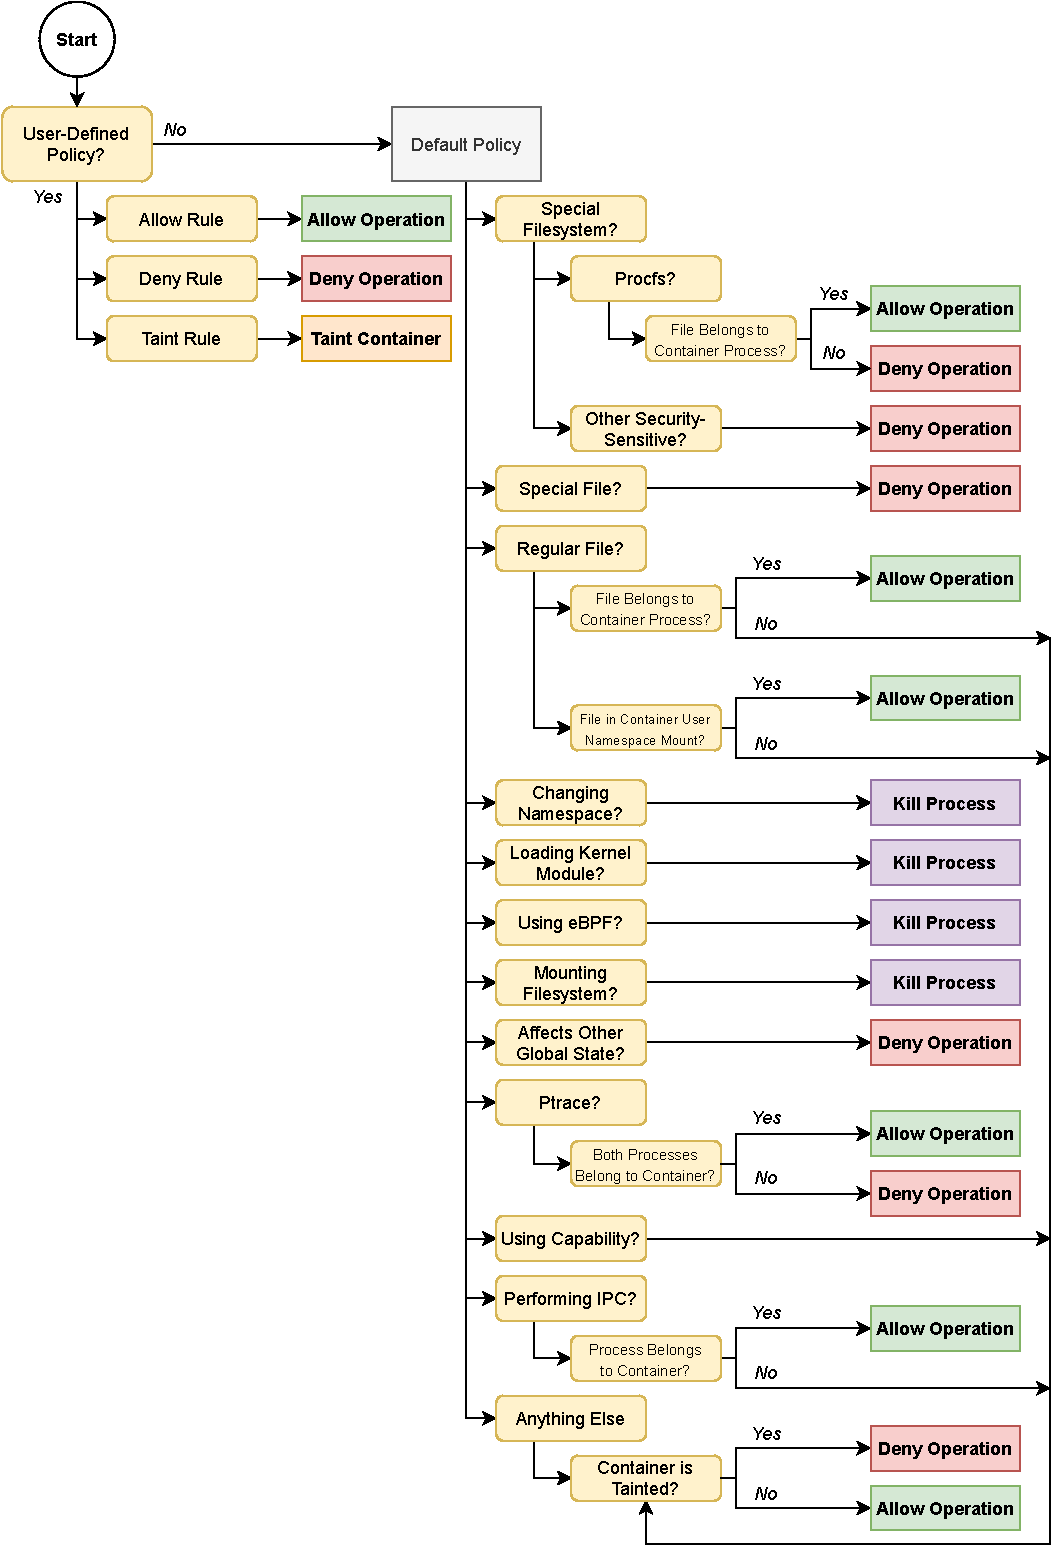
\includegraphics[width=0.75\linewidth]{figs/bpfcontain/enforcement.pdf}
  \caption[The policy enforcement strategy under \bpfcontain{}]{
    The policy enforcement strategy under \bpfcontain{}, expressed as a flowchart. Using
    container semantics, \bpfcontain{} achieves rich policy defaults, denying access to
    global resources and operations which can affect global system state while preserving
    intra-container access. This greatly simplifies the resulting confinement policy and
    enables the user to focus on specific exceptions to default protection.
  }\label{fig:bpfcontain-enforcement}
\end{figure}

\bpfcontain{}'s default policy depends largely on the type of access that a container is
requesting. If the requested access is to a regular file, \bpfcontain{} checks to see if
this file exists under the container's user namespace, provided that this namespace is
non-global. This covers, for example, a temporary or overlay filesystem mounted within
a non-global user namespace.  Similarly, default \gls{ipc} access is gated by whether or
not the processes on either end of the \gls{ipc} handle belong to the same container. If
they do, access is granted; otherwise, access is denied. Ptrace is similarly restricted;
a process may only ptrace another if both processes exist in the same container. In this
way, we preserve the semantics of the container: resources that exist \textit{within}
a container are accessible by processes within the same container, but resources
that exist \textit{without} are not be accessible by default.

Special files such as character or block devices are treated separately from regular
files. Since these provide direct interfaces into the kernel, it does not make sense to
treat them with the same semantics. Instead, access to special files is \textit{always}
denied, unless they are covered by an explicit \texttt{allow} rule. Similar protections
are applied to security-sensitive special filesystems such as \texttt{procfs},
\texttt{sysfs}, \texttt{securityfs}, and others. These filesystems are responsible for
exposing direct interfaces into the kernel, often with the ability to manipulate
behavioural parameters. For these special filesystems, \bpfcontain{} also always assumes
a default-deny policy, except in cases that are explicitly covered by an \texttt{allow}
rule. The only major exception to this policy is in the case of per-process entries
exposed by \texttt{procfs}; in this case, \bpfcontain{} assumes default allow provided
that the corresponding process is a member of the container.

An implicit assumption underlying \bpfcontain{}'s default enforcement strategy is that
a container is unable to mutate its namespace membership or manipulate its view of the
filesystem in any way. To ensure this, \bpfcontain{} strictly prohibits a container from
altering its namespace membership using an Fentry probe on the kernel's
\texttt{switch\_task\_namespaces()} function. Similarly, \bpfcontain{} prohibits
a container from ever mounting a new filesystem after starting confinement. In both cases,
violating this policy results in immediate delivery of \texttt{SIGKILL} to the offending
process.

Another underlying assumption is that a container cannot interfere with \bpfcontain{}'s
normal operation. Without this assumption, \bpfcontain{} would be unable to enforce any
security guarantees whatsoever, as an attacker could trivially bypass or disable it. To
enforce this, \bpfcontain{} prohibits a container from ever loading code into the kernel
or interacting with \gls{ebpf}. This design choice makes practical sense from a container
security perspective, as a confined container should not be able to load code into the
kernel to begin with\,---\,otherwise, escaping confinement would be trivial, as an
adversary could simply bypass the protection mechanism enforced by the kernel. As with
namespace and mount policy, violating these restrictions results in the immediate delivery
of an uncatchable \texttt{SIGKILL}.

Some \gls{ebpf}-based monitoring suites (e.g.~Cilium~\cite{cilium} and
Tracee~\cite{tracee}) are delivered as containers. Since \bpfcontain{} currently prohibits
\gls{ebpf} usage by a container, it would be a poor choice for confining these suites.
Future iterations on \bpfcontain{} may support confining containers with access to
\gls{ebpf}, although this would require \bpfcontain{} to protect its own programs and maps
using finer-grained policy defaults for the \texttt{bpf(2)} code path.

Aside from the aforementioned defaults, \bpfcontain{} also denies other miscellaneous
operations that can affect global state, including rebooting the system, attempting to
modify global system time, access to the kernel keyring, and access to the kernel's perf
events subsystem. Using a capability that has not been expressly marked with
an \texttt{allow} rule is considered default-deny. Any other access is considered
default-deny, if the container has been tainted.

\subsubsection{Future Improvements to Default Policy}\label{sss:bpfcontain-improving-default}

Presently, a major limitation of \bpfcontain{}'s approach to default filesystem policy is
that it relies on a container being in its own user namespace in order for default-allow
access to be considered. If a filesystem exists in the container's mount namespace but
does not belong to its user namespace, \bpfcontain{} must assume default-deny. However,
most container management systems, including Docker~\cite{docker_security}, do not run
containers under a new user namespace by default, meaning that \bpfcontain{} would be left
unable to use its default filesystem policy to grant access. While it is possible to force
Docker to run a container in a new user namespace, it would be beneficial if
\bpfcontain{}'s default policy would work regardless of user namespace membership.

There are a few technical challenges surrounding this idea, but it should be possible to
achieve in the future once \bpfcontain{} has been more integrated with Docker
(c.f.\ \Cref{ss:disc-docker-integration} in \Cref{c:discussion}). In particular, we can use
\gls{ebpf} uprobes and kfunc probes to trace Docker's \texttt{containerd} shim as it switches
namespaces and mounts the appropriate filesystems. We could then incorporate these
filesystems directly into \bpfcontain{}'s default policy without relying on user
namespace information provided by the kernel. Exploring this option is left as future work.

Another major technical issue underlying \bpfcontain{}'s default filesystem policy is that
the Linux overlay filesystem currently performs permission checks on the underlying inode
(from the original filesystem), rather than the overlayfs inode. This currently makes it
impossible to enforce \bpfcontain{}'s default filesystem policy on overlay filesystems,
which are generally used to implement the majority of a container's filesystem layout.  To
rectify this, we can leverage more \gls{ebpf} programs to trace the underlying overlay
filesystem operations and temporarily manipulate \bpfcontain{}'s state model to account
for this. This may add modest overhead to overlayfs operations. Like Docker integration,
we leave this for future work.

\subsection{Managing Container State}\label{ss:bpfcontain-state}

Like \bpfbox{}, \bpfcontain{} tracks the association of processes with policy profiles,
along with other state. However, under \bpfcontain{}, this state-tracking happens
at the level of individual containers rather than individual processes\,---\,we are
concerned with \textit{groups of processes}, associated by a shared sense of
virtualization and confinement. Tracking state at the level of containers rather than
individual processes is a major enabling factor behind \bpfcontain{}'s nuanced policy
defaults, as described in \Cref{ss:bpfcontain-default}.

To start tracing a container, \bpfcontain{} relies on the \texttt{bpfcontain-run} shim to
provide its kernelspace programs with basic information about which confinement policy to
associate with the container. Specifically, we care about the desired policy ID, a unique
64-bit integer associated with each \bpfcontain{} policy. In addition to a policy ID,
\bpfcontain{} generates a unique container ID for the container, a combination of a 32-bit
random integer and the 32-bit process ID of the container's \textit{init} process.
\bpfcontain{} maintains a hash map, mapping a container ID to a policy ID, to track the
association of a container with a confinement policy.

In addition to policy association, \bpfcontain{} tracks other metadata about the
container, including namespace membership, a reference count of how many processes are
running under the container, whether the container has been \textit{tainted}, and whether
the container is running in \textit{complaining mode}\footnote{Recall that complaining
mode causes \bpfcontain{} to log would-be denials without actually denying the
operation.}. These metadata are associated with using an \gls{ebpf} hash map with a simple
data structure as a map value and the container ID as the key. Namespace membership is
determined at runtime by taking the namespace IDs associated with the container's
\textit{init} process' task struct.

To manage container membership, \bpfcontain{} maintains a security blob in each
containerized task\footnote{A task is a Linux kernel data structure that represents a unit of
scheduling (i.e.~a process or a thread). \bpfcontain{} tracks processes and threads
individually at the per-task level.} using a task local storage map. Each task is
associated with a given container ID. When a task makes a request to a sensitive resource,
\bpfcontain{} makes a chain of map lookups, querying the task's container ID from the
local storage map, then using this container ID to query the associated policy ID. When
a task forks itself, \bpfcontain{} looks up its container membership and applies the same
membership to the child task, incrementing the container's reference count. When a task
exits, \bpfcontain{} simply decrements the container's reference count, cleaning up the
container when its reference count reaches zero. Any task-specific metadata is
automatically cleaned up by the local storage map.

\subsection{Collecting and Logging Audit Data}\label{ss:bpfcontain-audit}

While \bpfcontain{} does not expressly define audit rules, it still uses logging to record
any policy decisions to a file for subsequent analysis. To achieve this, \bpfcontain{}
uses the same strategy as \bpfbox{}, relying on a ring buffer map to pass events to
userspace for further treatment. Using this ring buffer, \bpfcontain{} achieves efficient,
in-order event logging across all \glspl{cpu}. Like \bpfbox{}, \bpfcontain{} supports
placing a container into a \textit{complaining mode}, enabling it so log denials that
would have happened while still granting access. This enables a policy author to test
their policy before running it in production and may be used to accommodate log-based
policy generation in the future.



\section{\bpfcontain{} Policy Language}\label{s:bpfcontain-policy}

This section presents the \bpfcontain{} policy language in detail. In particular, we
document the policy language schema and offer some insight into how rules can be used to
define exceptions to \bpfcontain{}'s default enforcement. Due to the modular design of
\bpfcontain{}'s policy deserializer, it supports a number of different serialization
formats to encode policy. In particular, YAML, TOML, and JSON are currently supported,
with the possibility to add others in the future. For the purposes of this section, we
assume the YAML format for consistency and readability.

\bpfcontain{} policies are stored in a central, root-controlled directory. At runtime, the
daemon watches policy files for changes and parses and loads the policy into the kernel
when updates occur. At a minimum, each \bpfcontain{} policy contains some metadata,
including the policy name and a few tunable parameters. Tunables include the ability to
mark a container as pre-tainted and the ability to specify a command to use as the default
entry point for \texttt{bpfcontain-run}. A pre-tainted container spawns tainted rather than
untainted, falling back to stricter defaults when no rule matches the requested access
(c.f.\ \Cref{fig:bpfcontain-enforcement} on page \pageref{fig:bpfcontain-enforcement}).

Aside from policy metadata, the policy is divided into three sections: allow, deny, and
taint. Each of these sections specifies the corresponding policy decision for any rules
declared within. When the \bpfcontain{} enforcement engine matches on a rule, it takes the
rule's policy decision as an enforcement action. In turn, policy rules are divided into
several categories based on the type of access that they specify. The subsections that
follow examine and document each supported rule category.

Note that, unlike \bpfbox{}, \bpfcontain{} does not currently support the ability to
define function-level policy. The rationale for this design choice is that
hyper-fine-grained policy makes little sense in the context of a container, particularly
considering \bpfcontain{}'s highly-nuanced policy defaults. Future work may involve
examining this design choice, along with other aspects of the \bpfcontain{} policy
language design, in the context of a user study (see the discussion
in~\Cref{c:discussion}). \Cref{lst:bpfcontain-policy-example} depicts an example
\bpfcontain{} policy for a simple remote login program.

\begin{lstlisting}[language=yaml, gobble=4,
  caption={[An example \bpfcontain{} policy  written in YAML]
    An example \bpfcontain{} policy for a simple remote login program, written in YAML.
    This example offers a fairly complete idea of the \bpfcontain{} policy language's
    various features.
The reader is encouraged to compare
    this policy with the policy depicted in \Cref{lst:bpfbox-policy-example} on page
    \pageref{lst:bpfbox-policy-example}.
  },
  label={lst:bpfcontain-policy-example}, float]
    # Name of the policy
    name: mylogin
    # Container entrypoint
    cmd: /usr/bin/mylogin
    # Spawn container untainted
    defaultTaint: false

    allow:
      # Perform send/recv operations as a client
      - net: [client, send, recv]
      # Grant read and append access to /etc/passwd
      - file: {pathname: /etc/passwd, access: ra}
      # Grant read-only access to /etc/shadow
      - file: {pathname: /etc/shadow, access: r}
      # Grant read and append access to any immediate child of /var/log/mylogin
      - file: {pathname: /var/log/mylogin/*, access: ra}
      # Grant read and execute access to bash
      - file: {pathname: /bin/bash, access: rx}
      # Grant read/write access to the TTY
      - dev: terminal

    taint:
      # Taint after performing any network operation
      - net: any
\end{lstlisting}

\subsection{File and Filesystem Rules}

For specifying access to regular files, \bpfcontain{} supports two major rule types.
\textit{File rules} specify access at the granularity of individual files while
\textit{filesystem rules} specify access at the granularity of a filesystem.  These may be
combined to grant or restrict coarse-grained access to entire filesystems and define
fine-grained exceptions to this coarse-grained access for specific files. These rules are
necessary since not every \bpfcontain{} policy targets an application running in
a container, and containers often access files directly from the host filesystem
(e.g.~through a Docker volume mount). Each file and filesystem rule consists of a pathname
and an access pattern. In the case of filesystem rules, the given pathname must be the
mountpoint of the filesystem. \bpfcontain{} supports several access flags for fine-grained
control over file access. \Cref{tab:bpfcontain-file-access} describes each flag and its
corresponding effect.

\begin{table}[htbp]
  \centering
  \caption[File access flags in \bpfcontain{}]{
    File access flags in \bpfcontain{}.
  }\label{tab:bpfcontain-file-access}
  \begin{tabular}{ll}
  \toprule
  Pattern & Access \\
  \midrule
  \texttt{r} & Read (\texttt{read(2)}, \texttt{getattr(2)}, etc.) \\
  \texttt{w} & Write (\texttt{write(2)}, \texttt{setattr(2)}, etc.)\\
  \texttt{a} & Append (\texttt{write(2)} with append-only flag set) \\
  \texttt{x} & Execute (\texttt{execve(2)})\\
  \texttt{m} & Map executable memory (\texttt{mmap(2)}) \\
  \texttt{c} & Modify Unix \gls{dac} (\texttt{chmod(2)}/\texttt{chown(2)}) \\
  \texttt{d} & Unlink/delete a file \\
  \texttt{l} & Create a hard link to a file \\
  \texttt{i} & Make an \texttt{ioctl(2)} call on a device \\
  \bottomrule
  \end{tabular}
\end{table}

When loading a file rule into the kernel, \bpfcontain{} translates the pathname into
a list of tuples uniquely describing the file. Each tuple contains the file's inode number
along with the unique device ID associated with the filesystem on which the inode resides.
These two numbers taken together can uniquely identify any file on the system.
\bpfcontain{}'s file rules similarly take the device ID of the filesystem root, ignoring
the inode. An implicit side effect of this technique is that files are immutably resolved
at policy load time, meaning that \bpfcontain{} can achieve pathname resolution without
becoming vulnerable to \gls{toctou} attacks. Like \bpfbox{}, \bpfcontain{} deals with
newly-created files by associating them with the task that created them, granting default
access to these files for the owning task\,---\,this resolves the use case where a task
requires access to a file created \textit{after} its policy has already been loaded.

\subsection{Device Rules}

Unlike \bpfbox{}, \bpfcontain{} takes great care to avoid conflating regular files and
special files. The key insight underlying this design choice is that the semantics of
regular files and special files are quite different, despite supporting fundamentally the
same operations. Provisioning over-permissive access to the wrong special file
(e.g.\ \texttt{/dev/mem}, which provides access to the system memory map) can have
devastating security consequences. For this reason, access to a special file must be
specified via a \textit{device rule} using the \lstinline[language=yaml]|dev| keyword,
rather than the \lstinline[language=yaml]|file| or \lstinline[language=yaml]|filesystem|
keywords.

\bpfcontain{} supports several major classes of character device, each with a default
access pattern according to the device's semantics.  For instance
\lstinline[language=yaml]|dev: terminal| enables read and write access on
\texttt{/dev/tty} to support standard input and output to the terminal. Likewise,
\lstinline[language=yaml]|dev: random| grants read only access to \texttt{/dev/random} and
\texttt{/dev/urandom}. When loading a device rule into the kernel, \bpfcontain{} resolves
the device's major and minor number pair and maps it to the corresponding access pattern.

More nuanced device access patterns may be specified using a numbered device rule,
specified as \lstinline[language=yaml]|numberedDev: {major: major, minor: minor, access: access}|
where \textit{major} and \textit{minor} are the device's major and minor number,
and \textit{access} is an access flag pattern. This access pattern uses the same file
access flags as outlined in \Cref{tab:bpfcontain-file-access}. The minor number is
optional and may be omitted to match \textit{any} device of the specified major number.
Note that modern kernels dynamically allocate their major and minor number, meaning that
it is possible for \bpfcontain{} to lose track of the association between these numbers
and the underlying device driver.  We acknowledge this limitation in
\Cref{s:eval-security} and describe how the \bpfcontain{} prototype can be trivially
modified to address it.

\subsection{Network Rules}

\bpfcontain{} simplifies \bpfbox{}'s network policy by categorizing network accesses into
high-level use cases rather than the underlying socket operations themselves. This
approach is informed by the insight that specific applications tend use specific sets of
socket operations, depending on if the application is designed as a client, a server, or
some combination of the two (e.g.\ a peer-to-peer model). Specifically, a server would
require the ability to create sockets, bind them to an \gls{ip} address, listen for and
accept incoming connections, and shut down existing connections. Conversely, a client
generally needs to connect to an existing bound socket. We further partition access by
provisioning send and receive access separately. \Cref{tab:bpfcontain-network} provides an
overview of these access categories.

\begin{table}[htpb]
  \centering
  \caption[Network access categories in \bpfcontain{}]{
    Network access categories in \bpfcontain{}. By combining the \texttt{client} or
    \texttt{server} keywords with the \texttt{send} and \texttt{recv} keywords, a policy
    can specify the correct level of access to required TCP socket operations.
  }\label{tab:bpfcontain-network}
  \begin{tabular}{ll}
  \toprule
  Category & Access \\
  \midrule
  \texttt{server} & Create, bind, listen, accept, and shut down socket connections \\
  \texttt{client} & Connect to a bound socket \\
  \texttt{send} & Send data over the socket \\
  \texttt{recv} & Receive data over the socket \\
  \bottomrule
  \end{tabular}
\end{table}

\bpfcontain{}'s network policy covers \gls{ip}v4 and \gls{ip}v6 sockets. Netlink and raw
packet sockets are prohibited by default, and Unix domain sockets are relegated to
\gls{ipc} rules rather than network rules (c.f.\ \Cref{ss:bpfcontain-ipc}).

\subsection{\glsentryshort{ipc} Rules}\label{ss:bpfcontain-ipc}

In general, container \gls{ipc} policy is handled by \bpfcontain{}'s default enforcement,
which permits \gls{ipc} between two processes provided that they belong to the same
container. All other instances of \gls{ipc} are denied by default. In cases where
inter-container \gls{ipc} is required, \bpfcontain{} provisions \gls{ipc} rules which are
defined as \lstinline[language=yaml]|ipc: name| where \textit{name} is the name of another
\bpfcontain{} policy. In order for inter-container \gls{ipc} to be allowed, both policies
must mutually grant each other \gls{ipc} access. This ensures that any communication
between containers is mutually authorized, preventing attackers from bypassing the
security assumptions of a policy. \bpfcontain{}'s \gls{ipc} rules cover all canonical
forms\footnote{However, \bpfcontain{} does not currently support fine-grained access
control over TCP/IP sockets. This is left as future work (see \Cref{s:disc-future-work}).}
of \gls{ipc} available on the system, including signals, System V \gls{ipc} objects, and
Unix domain sockets.

\subsection{Capability Rules}

Since container execution models can be (and often are) privileged by default,
\bpfcontain{} takes great care to be distrustful of any POSIX capabilities assigned to the
container. Specifically, \bpfcontain{} denies the use of \textit{any} POSIX capabilities
as part of its default policy. While this is a simple and highly effective strategy for
limiting the privileges of containers running under root's \gls{uid}, some container use
cases require additional privileges to correctly function. To accommodate these use cases,
\bpfcontain{} provisions a \textit{capability rule} which can be used to specify allowed
capabilities. The capability rule is specified using \lstinline[language=yaml]|capability: [capabilities...]|
where \textit{capabilities} is a list of POSIX capabilities.

Note that capability rules \textit{do not grant} additional capabilities to a container;
rather they are a mask over the set of all capabilities that a container can ever possess.
In particular, this means that a container must already have the corresponding capability
under the traditional POSIX capabilities model in order to be able to use it. Thus,
capability rules merely add an extra level of protection on top of the existing model,
preventing overprivilege by restricting the bounding capability set.


\section{Improvements Over \bpfbox{}}\label{s:bpfcontain-improvements}

As a successor to \bpfbox{}, \bpfcontain{} makes several fundamental improvements in terms
of dependency overhead, policy language simplification, and container-specific extensions.
This section summarizes some of these improvements in light of the implementation details
discussed earlier in this chapter.

\subsection{Minimizing Runtime Dependencies}\label{ss:bpfcontain-minimizing}

\bpfcontain{} solves \bpfbox{}'s dependency and runtime overhead issues by leveraging Rust
and libbpf \gls{core}~\cite{nakryiko2020_core} rather than Python and bcc.  Unlike bcc,
libbpf \gls{core} enables \gls{bpf} programs to be compiled once and run anywhere, thanks
to \gls{btf} information provided by the kernel and load-time symbol relocation. Program
bytecode can then be embedded directly into the compiled object file, meaning the single
pre-compiled \bpfcontain{} binary can be deployed on any target kernel that meets
a minimal set of requirements. As a side effect, \bpfcontain{} requires neither a full
LLVM toolchain nor kernel headers to be available in the target deployment.

Moreover, implementing the \bpfcontain{} daemon in Rust allows \bpfcontain{} to take
advantage of a myriad of benefits offered by the Rust language. In particular, Rust
enables \bpfcontain{}'s userspace components to be safe, secure, and fast. Thread and
memory safety guarantees provided by Rust ownership model eliminate many common security
bugs including memory corruption vulnerabilities and race conditions between threads.
These safety guarantees provide critical security advantages, particularly given the fact
that the \bpfcontain{} daemon is a long-running, privileged process\,---\,a ripe target
for attacker exploitation. Thanks to an emphasis on speed and zero-cost abstractions, Rust
can provide these benefits at virtually zero overhead, in line with traditional systems
programming languages like C and with significantly smaller overhead than interpreted
languages such as Python.

\subsection{Improved Policy Language}\label{ss:bpfcontain-simplified}

\bpfcontain{} greatly simplifies the original \bpfbox{} policy language. Rather than
defining a specific policy language syntax, \bpfcontain{} defines a schema that can be
encoded in multiple different data serialization languages.  This simultaneously enables
\bpfcontain{} to support a policy language that users are already familiar with (e.g.\ YAML)
and provides a clear path for extending \bpfcontain{} to support additional policy
languages in the future. Further, this approach presents an opportunity for integrating
\bpfcontain{} policy with existing specifications, such as the \gls{oci} specification or
the rego~\cite{rego} policy framework, both of which are encoded in JSON\@. Integrating
with the \gls{oci} specification will enable \bpfcontain{} policies to be specified
directly within container manifests. Integrating with rego would enable \bpfcontain{}
policies to interact with the Open Policy Agent, widely used to implement policy in the
Kubernetes container orchestration framework.

Further simplifications to the \bpfcontain{} policy language are afforded by its goal of
container-specific confinement. By focusing on container-specific use cases,
\bpfcontain{}'s default policy enforcement can be far more nuanced than a traditional
sandboxing framework. This property enables the user to focus on defining specific
exceptions to a well-defined security boundary rather than enumerating every single
possible resource that a container can access. Along with the simplifications afforded by
\bpfcontain{}'s sensible policy defaults, we make additional changes to the policy
language that help decouple it from the underlying details of the operating system, such
as higher-level network policy and semantically-guided device driver access defaults.

Moreover, \bpfcontain{} improves upon the original \bpfbox{} policy language design by
introducing new rule types to cover weaknesses in the original design. It also fully
implements many aspects of \bpfbox{} that were left unfinished in the current
implementation, providing a more fully realized prototype. For these reasons,
\bpfcontain{} deprecates \bpfbox{} by implementing a superset of its original
functionality and improving upon flaws in the original \bpfbox{} design.



\subsection{Container-Specific Extensions}\label{ss:bpfcontain-extending}

Perhaps the most significant improvement over the original \bpfbox{} design is that
\bpfcontain{} implements container-specific confinement. Whereas \bpfbox{} is well suited
to fine grained, process level confinement, \bpfcontain{} extends this design to model
containers. In particular, \bpfcontain{} tracks namespace membership as well as the
association between processes and containers, enabling access to resources within
a container and restricting access to the outside world. This approach is similar in
spirit to FreeBSD Jails~\cite{kamp2000_jails}. Unlike Jails, however, the \bpfcontain{}
implementation applies such container specific defaults without any changes to the
upstream kernel.

\bpfcontain{}'s container-specific extensions enable \bpfcontain{} to enforce
container-level policy with a well-defined security boundary around the container,
simultaneously improving security and greatly simplifying the resulting policies. Rather
than focusing on each and every resource associated with the container, security policies
can instead focus on defining exceptions in \bpfcontain{}'s security boundary, resulting
in policies that closely mirror the exposed interface to the outside world.






\section{Summary}\label{s:bpfcontain-summary}

This chapter has presented the design and implementation of \bpfcontain{}, an extension on
top of the original \bpfbox{} design that promotes container-specific confinement and uses
container semantics to simplify policies while providing strong security guarantees.
Using \gls{ebpf}, \bpfcontain{} supports container-level semantics in a kernel-level
enforcement engine without sacrificing adoptability or tying the kernel down to a specific
definition of a container. \bpfcontain{} uses these container-level semantics to define
a clear protection boundary around containers and provides a simple policy language for
defining exceptions to this protection boundary.

\chapter{Evaluation}\label{c:evaluation}
This chapter presents an evaluation of \bpfbox{} and \bpfcontain{} in terms of their
performance and security. \Cref{s:eval-performance} presents the methodology and results
of a performance evaluation involving micro- and macro-benchmarking of \bpfbox{} and
\bpfcontain{}. Results are compared with AppArmor~\cite{cowan2000_apparmor}, a popular
\gls{lsm} framework for \gls{mac} security policy. Finally, \Cref{s:eval-security}
presents a security analysis of \bpfbox{} and \bpfcontain{} under the threat model
outlined in \Cref{s:cp-threat-model}.

\section{Performance Evaluation}\label{s:eval-performance}

This section presents a performance evaluation of \bpfbox{} and \bpfcontain{}, measuring
their performance overhead using a variety of micro- and macro-benchmarking tests. In
particular, we use the Phoronix Test Suite~\cite{phoronix} to measure overhead across
a variety of computational tasks, workloads, and kernel interfaces. Each of these
benchmarks exercises a different subset of \bpfbox{} and \bpfcontain{}'s enforcement
engine, providing an approximation of their impact on the overall system. We also measure
the performance of the base system as a control and the performance overhead of AppArmor
as a basis for direct comparison. The subsections that follow provide an overview of our
testing methodology and present the benchmark results.

\subsection{Methodology}\label{ss:eval-methodology}

As a test environment, we utilize a bare-metal system running Arch Linux with a stock
5.12.14-arch-1-1 kernel. The choice of a bare-metal system (rather than a virtual machine,
for instance) reduces the risk of introducing additional sources of variance into the
benchmarks. \Cref{tab:system-config} provides a detailed account of the test system
configuration.

\begin{table}[htp]
  \centering
  \footnotesize
  \caption[System configuration for benchmarking tests]{System configuration for benchmarking tests.}\label{tab:system-config}
  \begin{tabular}{ll}
  \toprule
  Item & Description / Configuration \\
  \midrule
  CPU & Intel i7-10875H; 8 cores, 16 threads at 2.3GHz; 16MB cache\\
  GPU & Nvidia RTX 2060 with 6GB GDDR6 VRAM \\
  RAM & 2$\times$16GB DDR4 at 3.2GHz \\
  Disk & 1TiB Samsung NVME M.2 SSD \\
  Motherboard & System76 oryp6 \\
  \midrule
  \gls{os} & Arch Linux (Rolling) \\
  Kernel & Linux v5.12.14-arch-1-1 \\
  Libc & glibc v2.33-5 \\
  Phoronix & v10.4.0-1 \\
  \bottomrule
  \end{tabular}
\end{table}

To simulate the Docker container use case, we run all tests in a privileged Docker
container, using Docker volumes to mount the host filesystem in the benchmarking
directory. To improve benchmarking accuracy, we also perform the following setup before
each test. (1) We disable SMT hyperthreading by turning off each logical CPU core pair,
leaving only the physical cores active; (2) We disable turbo boost, capping the CPU at its
stock speed of 2.3GHz; (3) We set the CPU frequency scaling governor to
\enquote{performance} to limit the impact of thermal throttling and power saving features;
and (4) We globally disable \gls{aslr} by setting the appropriate kernel parameter. These
settings, consistent with best practices, improve benchmark accuracy by making the
environment more consistent and eliminating as many external factors as possible.

\begin{table}[htp]
  \centering
  \footnotesize
  \caption[List of benchmarking suites and what they measure]{
    A list of the benchmarking suites used to test performance overhead, and what each
    measures.
  }\label{tab:suites}
  \begin{tabular}{lll}
  \toprule
  Test Suite & Test & Measures \\
  \midrule
  OSBench                    & Create Files       & Time to create and delete files \\
                             & Create Threads     & Time to create new threads \\
                             & Launch Programs    & Time to fork + execve \\
                             & Create Processes   & Time to create new processes \\
                             & Memory Allocations & Memory allocation throughput \\
  Kernel Compilation         & ---                & Time to compile Linux Kernel \\
  Apache Web Server          & ---                & Apache HTTP request throughput \\
\bottomrule
  \end{tabular}
\end{table}

To measure the performance overhead of \bpfbox{} and \bpfcontain{} (compared with the base
system and with AppArmor) we use the Phoronix Test Suite~\cite{phoronix}, a popular
cross-platform benchmarking framework that has seen wide use for measuring system
performance. The Phoronix framework comprises a number of open source test suites, each
targeting a different aspect of system behaviour. For the purposes of this thesis, we
select three separate test suites, measuring a variety of \gls{os}-level functionality and
exercising multiple \gls{lsm} hooks. In particular, we select the OSBench suite, the
Kernel Compilation suite, and the Apache suite. \Cref{tab:suites} describes each test
suite and what it measures.

\begin{figure}[htp]
  \centering
  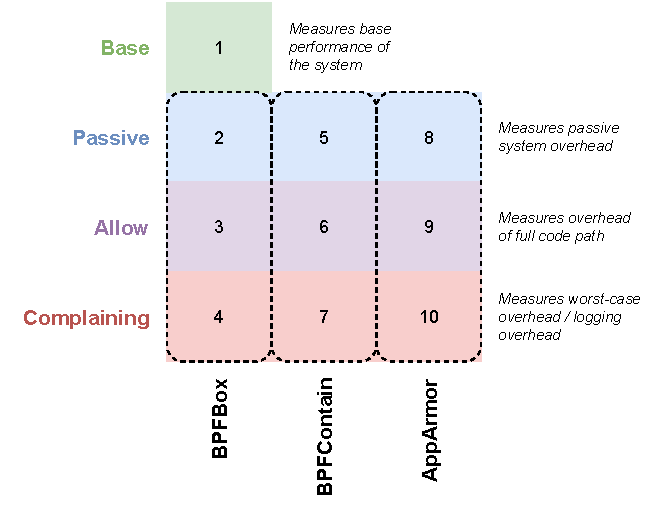
\includegraphics[width=0.8\linewidth]{figs/eval/configuration.pdf}
  \caption[Benchmarking system configurations]{
    The various system configurations used in the benchmarking tests.
    Each numbered cell constitutes one configuration, for a total of ten.
  }\label{fig:configuration}
\end{figure}

We consider ten system configurations in total (\Cref{fig:configuration}). The
\textbf{Base} configuration is the base system without any \glspl{lsm} or other
confinement primitives active or loaded in the kernel. The \textbf{\bpfbox},
\textbf{\bpfcontain}, and \textbf{AppArmor} configurations measure the performance
overhead of \bpfbox{}, \bpfcontain{}, and AppArmor, respectively. We then divide each of
these three configurations into three distinct test cases each. The \textbf{Passive} case
measures global system overhead without any active enforcement. The \textbf{Allow} case
measures active enforcement, allowing all security-sensitive operations. Finally, the
\textbf{Complaining} case measures the worst-case overhead for each system, exercising the
full code path of each \gls{lsm} hook and logging every attempted access.

To calculate percent overhead for each test configuration, we take the mean of all
test results for a given configuration and calculate the percent change from
the base configuration. This is done using the following formula:
$$
  \text{Percent Overhead} = \frac{\left(\bar{x}_{test} - \bar{x}_{base}\right)}{|\bar{x}_{base}|} \times 100
$$

To ensure statistically valid results, we run each test at least eleven times, until
a standard deviation of at most $2\%$ of the mean is achieved. The standard deviation
bound is a sensible default enforced by the Phoronix Test Suite to ensure statistically
valid results. We also discard the first run of each test to control for initial I/O
transients. In the end, no additional trials were necessary, as we were able to achieve
under $2\%$ standard deviation for all test configurations. For reproducibility, we make
the benchmarking repository publicly available\footnote{Benchmarking tests are available:
\url{https://github.com/willfindlay/bpfcontain-benchmarks}}, including all results and
related scripts.











\subsection{Results}\label{ss:eval-results}

This section presents the results of the OSBench micro-benchmarks (\Cref{fig:osbench} and
\Crefrange{tab:phoronix-create-files}{tab:phoronix-memory-allocations}), the kernel
compilation (\Cref{fig:phoronix-kernel} and \Cref{tab:phoronix-kernel-compilation}) and
Apache web server (\Cref{fig:phoronix-apache} and \Cref{tab:phoronix-apache})
macro-benchmarks. We find that \bpfbox{} and \bpfcontain{} incur modest overhead in many
common use cases cases, with \bpfcontain{} experiencing performance degradations in some
cases. Also, we discuss how future optimizations to \bpfcontain{} and the \gls{krsi}
framework could greatly improve its performance overhead in practice.

\begin{figure}[htp]
  \centering
  \subfloat{
    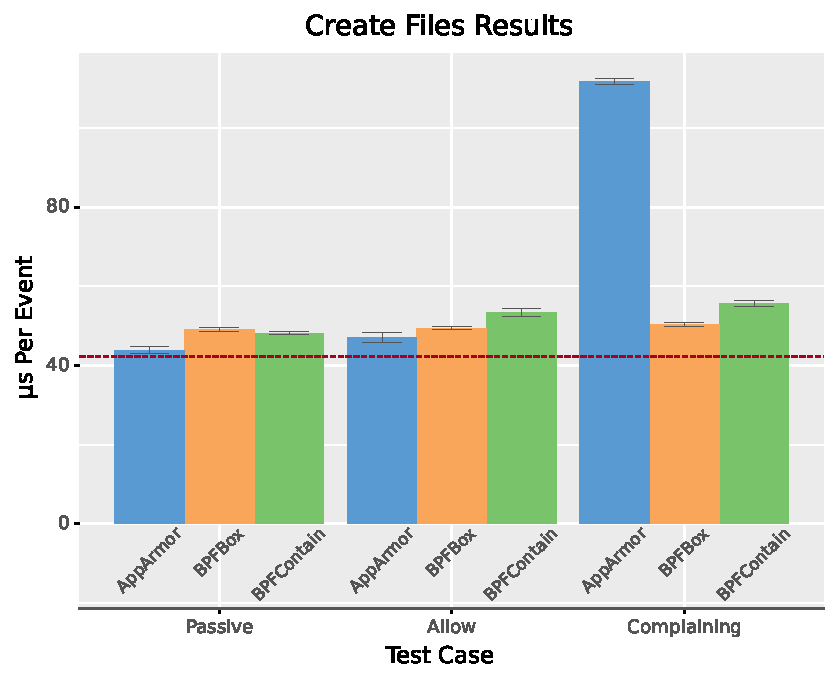
\includegraphics[width=0.45\linewidth]{results/graphs/Create-Files.pdf}}\qquad
  \subfloat{
    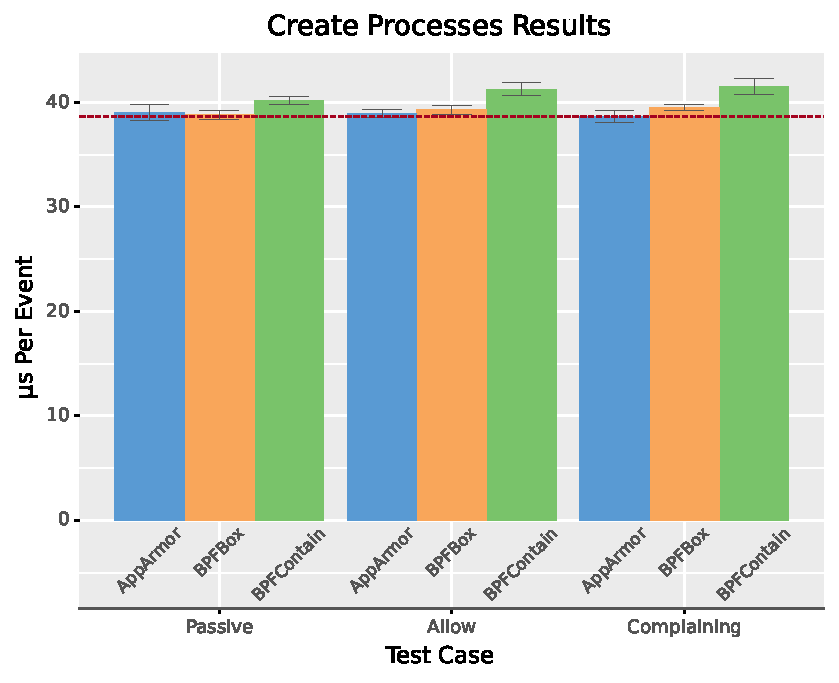
\includegraphics[width=0.45\linewidth]{results/graphs/Create-Processes.pdf}}\\
  \subfloat{
    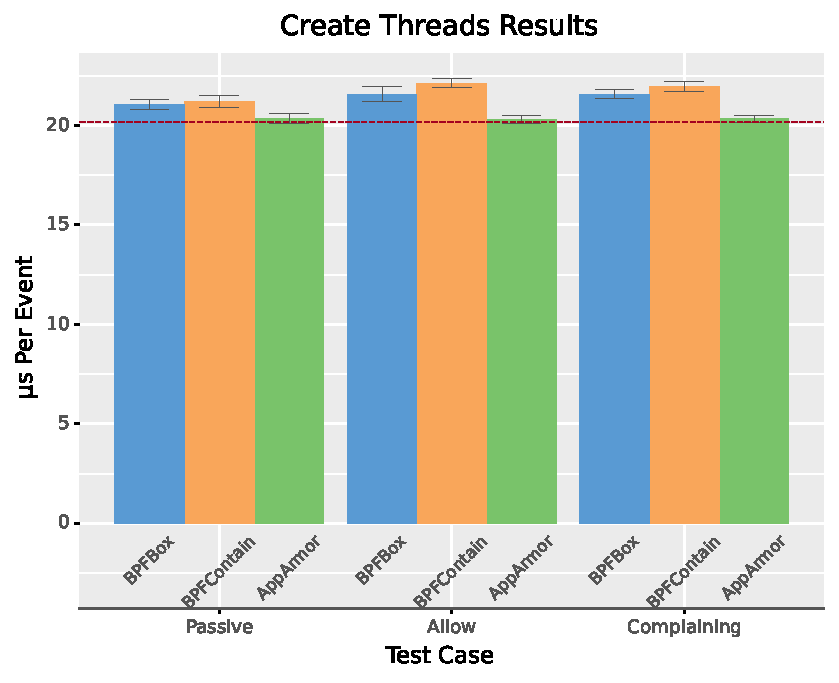
\includegraphics[width=0.45\linewidth]{results/graphs/Create-Threads.pdf}}\qquad
  \subfloat{
    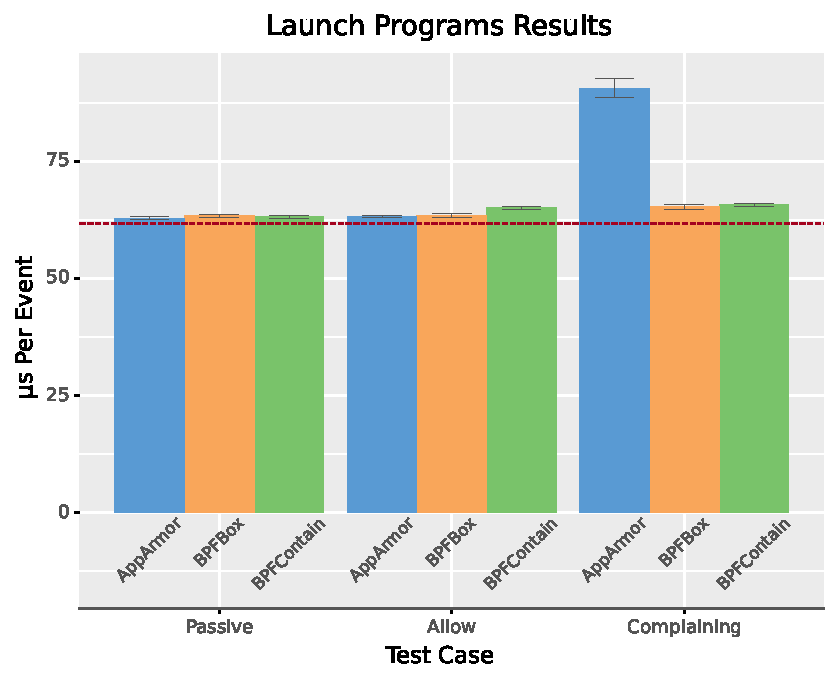
\includegraphics[width=0.45\linewidth]{results/graphs/Launch-Programs.pdf}}\\
  \subfloat{
    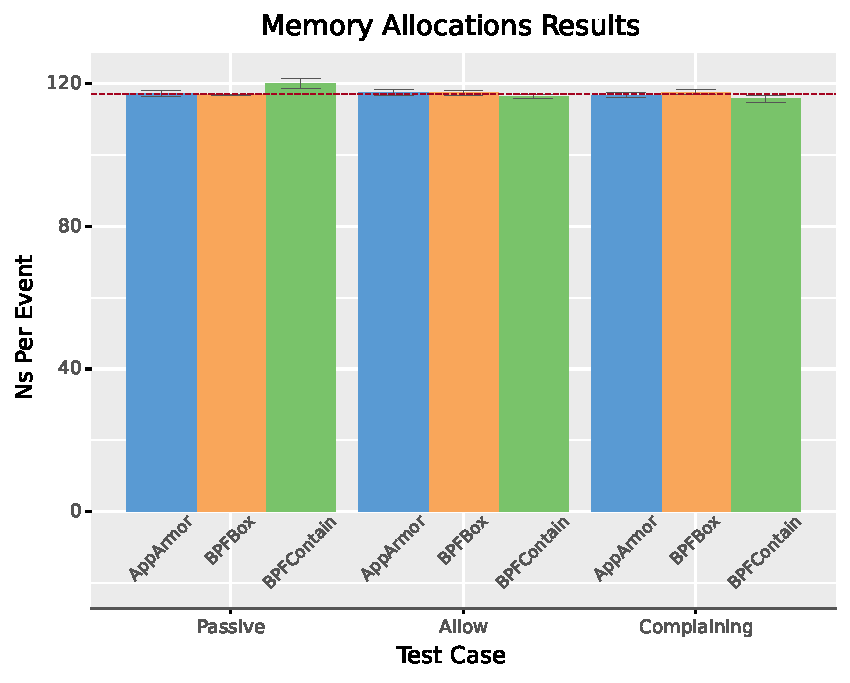
\includegraphics[width=0.45\linewidth]{results/graphs/Memory-Allocations.pdf}}
  \caption[The results of the OSBench micro-benchmarks]{
    The results of the OSBench micro-benchmarks. The error bars show standard
    deviation and the red lines show base measurements for each test. Lower times are
    better.
  }\label{fig:osbench}
\end{figure}

\subsubsection{OSBench File Creation}

The file creation benchmark (\Cref{tab:phoronix-create-files} and \Cref{fig:osbench})
indicates that \bpfbox{} and \bpfcontain{} have significantly higher overhead than
AppArmor in the \textbf{Passive} and \textbf{Allow} cases. \bpfcontain{}, in particular,
performs the worst out of the three systems in these two cases. It is perhaps unsurprising
that \bpfcontain{} performed worse on this test, since it performs complex analysis on
filesystem operations to come to a policy decision. We made no deliberate optimization
attempts in this research prototype, but expect that future performance improvements are
possible.  Conversely, AppArmor is a well-established security mechanism which has
undergone significant performance optimizations over time. Future optimizations on
\bpfcontain{} could likely improve its performance overhead in practice. Despite
a seemingly high performance overhead in the \textbf{Passive} and \textbf{Allow} cases,
\bpfbox{} and \bpfcontain{} incur a performance penalty of under 12$\mu$s each.  The
kernel compilation macro-benchmarks, presented later in this section
(c.f.\ \Cref{fig:phoronix-kernel} and \Cref{tab:phoronix-kernel-compilation}) indicate that
this slowdown has very little effect on even moderately complex workloads.  Moreover, in
the \textbf{Complaining} case, \bpfbox{} and \bpfcontain{} significantly outperform
AppArmor. This result can be attributed to implementation differences in their
event-logging mechanisms.

\begin{table}[ht!]
\centering
\footnotesize
\caption[Results of the Create Files benchmark]{Results of the Create Files benchmark. Units are $\mu$s per event. Lower is better. Percent overhead is compared to the baseline result.}
\label{tab:phoronix-create-files}
\begin{tabular}{llrrr}
\toprule
            &          &    Mean &   Std &  Overhead \\
Test Case & System &         &       &           \\
\midrule
Base & --- &   42.21 &  1.22 &       --- \\
\cline{1-5}
\multirow{3}{*}{Passive} & BPFBox &   49.09 &  0.40 &   16.31\% \\
            & BPFContain &   48.16 &  0.36 &   14.11\% \\
            & AppArmor &   43.87 &  0.95 &    3.93\% \\
\cline{1-5}
\multirow{3}{*}{Allow} & BPFBox &   49.41 &  0.39 &   17.08\% \\
            & BPFContain &   53.43 &  1.01 &   26.60\% \\
            & AppArmor &   47.07 &  1.15 &   11.52\% \\
\cline{1-5}
\multirow{3}{*}{Complaining} & BPFBox &   50.34 &  0.54 &   19.27\% \\
            & BPFContain &   55.67 &  0.75 &   31.89\% \\
            & AppArmor &  111.66 &  0.75 &  164.55\% \\
\bottomrule
\end{tabular}
\end{table}


In the \textbf{Passive} case, \bpfbox{} and \bpfcontain{}'s high performance overhead can
be attributed to the fact that they each invoke multiple \gls{bpf} programs over multiple
\gls{lsm} hooks on the \texttt{open(2)}, \texttt{write(2)}, and \texttt{unlink(2)} code
paths. Unlike AppArmor, \bpfbox{} and \bpfcontain{} invoke a new \gls{ebpf} program on
every \gls{lsm} hook along this code path and then perform a map lookup to determine whether
the process is being actively traced. The overhead associated with this many \gls{bpf}
program invocations is non-trivial compared with the overhead of simply calling into an
\gls{lsm} hook. Future improvements to the \gls{krsi} framework may also be able to reduce
the performance overhead of \gls{bpf} \gls{lsm} programs.

In the \textbf{Allow} case, \bpfbox{} is more in line with AppArmor, while \bpfcontain{}
is shown to exhibit a slightly higher overhead. We can attribute the additional
overhead shown by \bpfcontain{} to the nuances associated with its code path for file and
filesystem policies. For each file operation, \bpfcontain{} performs multiple map queries
and reads information from multiple kernel data structures to enforce its default policy.
Future iterations of \bpfcontain{} may improve this overhead by caching policy decisions
for filesystem objects and/or resolving inefficiencies in how \bpfcontain{} reads
information from kernel data structures.

In the \textbf{Complaining} case, \bpfbox{} and \bpfcontain{} significantly outperform
AppArmor, a fact which can be attributed to inefficiencies in AppArmor's logging
mechanism, which relies on the kernel's audit framework. The ring buffer maps used by
\bpfbox{} and \bpfcontain{} are known to exhibit comparatively less
overhead~\cite{zeng2015_auditing, zhang2021_lsm_file_overhead, nakryiko2020_ringbuf}.
Additional overhead may also arise due to differences in how AppArmor translates files and
access patterns to log messages.

\subsubsection{OSBench Process Creation}

The results of the process creation benchmark (\Cref{tab:phoronix-create-processes} and \Cref{fig:osbench}) indicate
that \bpfbox{} and \bpfcontain{} introduce modest overhead on top of the \texttt{fork(2)}
system call.  Comparatively, AppArmor introduces very little overhead, well within the
margin of error for measurements. The additional overhead introduced by \bpfbox{} and
\bpfcontain{} can be explained by the additional per-process and per-thread accounting
performed by each system. \bpfcontain{}, in particular, handles a significant amount of
per-process and per-thread metadata, which must be populated each time a \texttt{fork(2)}
or \texttt{clone(2)} occurs and cleaned up each time a process exits. However, it should
be noted that both \bpfbox{} and \bpfcontain{} introduce less than $10\%$ overhead along
this code path (within 1--2$\mu$s), which should be imperceptible in practice.

\begin{table}[ht!]
\centering
\footnotesize
\caption[Results of the Create Processes benchmark]{Results of the Create Processes benchmark. Units are $\mu$s per event. Lower is better. Percent overhead is compared to the baseline result.}
\label{tab:phoronix-create-processes}
\begin{tabular}{llrrr}
\toprule
            &          &   Mean &   Std & Overhead \\
Test Case & System &        &       &          \\
\midrule
Base & --- &  38.65 &  0.36 &      --- \\
\cline{1-5}
\multirow{3}{*}{Passive} & BPFBox &  38.81 &  0.44 &   0.40\% \\
            & BPFContain &  40.17 &  0.39 &   3.93\% \\
            & AppArmor &  39.04 &  0.74 &   1.01\% \\
\cline{1-5}
\multirow{3}{*}{Allow} & BPFBox &  39.28 &  0.41 &   1.63\% \\
            & BPFContain &  41.27 &  0.63 &   6.77\% \\
            & AppArmor &  38.94 &  0.34 &   0.74\% \\
\cline{1-5}
\multirow{3}{*}{Complaining} & BPFBox &  39.51 &  0.33 &   2.22\% \\
            & BPFContain &  41.49 &  0.76 &   7.33\% \\
            & AppArmor &  38.68 &  0.56 &   0.07\% \\
\bottomrule
\end{tabular}
\end{table}

\FloatBarrier



\subsubsection{OSBench Thread Creation}

The thread creation results (\Cref{tab:phoronix-create-threads} and \Cref{fig:osbench})
are directly related to the process creation results, insofar as both operations exercise
the same \gls{bpf} programs in \bpfbox{} and \bpfcontain{}. Since thread creation is
faster then process creation, the percentage overhead of \bpfbox{} and \bpfcontain{}
appear comparatively higher, but the underlying delta is the same, at roughly 1--2$\mu$s
per event. Despite these differences in thread and process creation speeds, the resulting
percentage overhead of \bpfbox{} and \bpfcontain{} is still under 10\%.



\begin{table}[ht!]
\centering
\footnotesize
\caption[Results of the Create Threads benchmark]{Results of the Create Threads benchmark. Units are $\mu$s per event. Lower is better. Percent overhead is compared to the baseline result.}
\label{tab:phoronix-create-threads}
\begin{tabular}{llrrr}
\toprule
            &          &   Mean &   Std & Overhead \\
Test Case & System &        &       &          \\
\midrule
Base & --- &  20.18 &  0.19 &      --- \\
\cline{1-5}
\multirow{3}{*}{Passive} & BPFBox &  21.06 &  0.25 &   4.37\% \\
            & BPFContain &  21.21 &  0.30 &   5.08\% \\
            & AppArmor &  20.32 &  0.25 &   0.71\% \\
\cline{1-5}
\multirow{3}{*}{Allow} & BPFBox &  21.56 &  0.37 &   6.84\% \\
            & BPFContain &  22.11 &  0.22 &   9.53\% \\
            & AppArmor &  20.29 &  0.18 &   0.54\% \\
\cline{1-5}
\multirow{3}{*}{Complaining} & BPFBox &  21.57 &  0.25 &   6.90\% \\
            & BPFContain &  21.96 &  0.24 &   8.80\% \\
            & AppArmor &  20.32 &  0.16 &   0.70\% \\
\bottomrule
\end{tabular}
\end{table}


\subsubsection{OSBench Program Launching}

The launch programs benchmark (\Cref{tab:phoronix-launch-programs} and \Cref{fig:osbench}) is essentially the
same as the process creation benchmark (c.f.\ \Cref{tab:phoronix-create-processes}), with one
major difference: the addition of an \texttt{execve(2)} call after the \texttt{clone(2)}
system call. This \texttt{execve(2)} call adds a constant overhead of about 20$\mu$s on
top of the original process creation results, as well as additional \gls{lsm} hook
invocations along the \texttt{execve(2)} code path. These factors contribute to \bpfbox{}
and \bpfcontain{} performing slightly worse than AppArmor in the \textbf{Passive} and
\textbf{Allow} cases and significantly better than AppArmor in the \textbf{Complaining}
case.

The additional \gls{lsm} hook invocations caused by the \texttt{execve(2)} severely impact
AppArmor's performance in the \textbf{Complaining} case for the same reasons as discussed
in the file creation results (c.f.\ \Cref{tab:phoronix-create-files}). \bpfbox{} and \bpfcontain{}
exhibit comparatively little overhead despite the \texttt{execve(2)} call. This result
can be explained by the fact that \texttt{execve(2)}'s code path invokes significantly
fewer \gls{lsm} hooks than the file creation and deletion code paths we examined earlier.
In all test cases, \bpfbox{} and \bpfcontain{} are able to achieve under $7\%$ overhead in
the worst case and under $3\%$ in the majority of cases.



\begin{table}[ht!]
\centering
\footnotesize
\caption[Results of the Launch Programs benchmark]{Results of the Launch Programs benchmark. Units are $\mu$s per event. Lower is better. Percent overhead is compared to the baseline result.}
\label{tab:phoronix-launch-programs}
\begin{tabular}{llrrr}
\toprule
            &          &   Mean &   Std & Overhead \\
Test Case & System &        &       &          \\
\midrule
Base & --- &  61.67 &  0.20 &      --- \\
\cline{1-5}
\multirow{3}{*}{Passive} & BPFBox &  63.30 &  0.28 &   2.64\% \\
            & BPFContain &  63.12 &  0.28 &   2.34\% \\
            & AppArmor &  62.84 &  0.25 &   1.89\% \\
\cline{1-5}
\multirow{3}{*}{Allow} & BPFBox &  63.44 &  0.40 &   2.86\% \\
            & BPFContain &  65.05 &  0.38 &   5.47\% \\
            & AppArmor &  63.17 &  0.21 &   2.43\% \\
\cline{1-5}
\multirow{3}{*}{Complaining} & BPFBox &  65.22 &  0.48 &   5.75\% \\
            & BPFContain &  65.66 &  0.30 &   6.47\% \\
            & AppArmor &  90.56 &  1.97 &  46.83\% \\
\bottomrule
\end{tabular}
\end{table}


\subsubsection{OSBench Memory Allocations}

The memory allocation benchmark (\Cref{tab:phoronix-memory-allocations} and
\Cref{fig:osbench}) indicates that none of the systems had any significant affect on
memory allocation. In some cases, percent overhead falsely appears to indicate
a performance \textit{improvement}, which we attribute to measurement error rather than
any indication of increased performance; all results from this trial were well within the
margin of error. This result is consistent with expectations since memory allocation does
not directly interact with any \gls{lsm} hooks in the kernel, and neither \bpfbox{} nor
\bpfcontain{} instruments any \gls{bpf} programs on the page allocation code path.

\begin{table}[ht!]
\centering
\footnotesize
\caption[Results of the Memory Allocations benchmark]{Results of the Memory Allocations benchmark. Units are ns per event. Lower is better. Percent overhead is compared to the baseline result.}
\label{tab:phoronix-memory-allocations}
\begin{tabular}{llrrr}
\toprule
            &          &    Mean &   Std & Overhead \\
Test Case & System &         &       &          \\
\midrule
Base & --- &  117.17 &  0.67 &      --- \\
\cline{1-5}
\multirow{3}{*}{Passive} & BPFBox &  116.87 &  0.18 &  -0.26\% \\
            & BPFContain &  120.05 &  1.27 &   2.46\% \\
            & AppArmor &  117.24 &  0.97 &   0.06\% \\
\cline{1-5}
\multirow{3}{*}{Allow} & BPFBox &  117.41 &  0.71 &   0.21\% \\
            & BPFContain &  116.42 &  0.62 &  -0.64\% \\
            & AppArmor &  117.49 &  0.81 &   0.28\% \\
\cline{1-5}
\multirow{3}{*}{Complaining} & BPFBox &  117.62 &  0.75 &   0.38\% \\
            & BPFContain &  115.73 &  1.04 &  -1.22\% \\
            & AppArmor &  116.81 &  0.80 &  -0.31\% \\
\bottomrule
\end{tabular}
\end{table}




\subsubsection{Kernel Compilation Results}

The kernel compilation benchmark (\Cref{tab:phoronix-kernel-compilation} and
\Cref{fig:phoronix-kernel}) provides a representative depiction of overhead for
a computationally-heavy task that involves multiple processes and significant amounts of
file I/O. The results of this benchmark indicate that \bpfbox{} and \bpfcontain{} exhibit
performance overhead that is roughly consistent with AppArmor in the average case. The
\textbf{Passive} and \textbf{Allow} results indicate that all three systems exhibit an
acceptable performance overhead of under about $3\%$. The \textbf{Complaining} results
indicate that \bpfcontain{} performs significantly better than both \bpfbox{} and AppArmor
under a large event logging volume. This result can be attributed to minor implementation
details, including improvements in how \bpfcontain{} handles event logging from multiple
distinct sources.


\begin{table}[ht!]
\centering
\footnotesize
\caption[Results of the Kernel Compilation benchmark]{Results of the Kernel Compilation benchmark. Units are seconds. Lower is better. Percent overhead is compared to the baseline result.}
\label{tab:phoronix-kernel-compilation}
\begin{tabular}{llrrr}
\toprule
            &          &    Mean &   Std & Overhead \\
Test Case & System &         &       &          \\
\midrule
Base & --- &  235.32 &  1.96 &      --- \\
\cline{1-5}
\multirow{3}{*}{Passive} & BPFBox &  237.95 &  1.88 &   1.12\% \\
            & BPFContain &  237.63 &  2.08 &   0.98\% \\
            & AppArmor &  236.45 &  1.92 &   0.48\% \\
\cline{1-5}
\multirow{3}{*}{Allow} & BPFBox &  238.23 &  2.19 &   1.24\% \\
            & BPFContain &  243.09 &  2.19 &   3.30\% \\
            & AppArmor &  237.59 &  2.04 &   0.97\% \\
\cline{1-5}
\multirow{3}{*}{Complaining} & BPFBox &  269.64 &  1.98 &  14.59\% \\
            & BPFContain &  244.80 &  2.04 &   4.03\% \\
            & AppArmor &  288.54 &  2.11 &  22.62\% \\
\bottomrule
\end{tabular}
\end{table}

\begin{table}[ht!]
\centering
\footnotesize
\caption[Results of the Apache benchmark]{Results of the Apache benchmark. Units are requests per second. Higher is better. Percent overhead is compared to the baseline result.}
\label{tab:phoronix-apache}
\begin{tabular}{llrrr}
\toprule
            &          &      Mean &     Std & Overhead \\
Test Case & System &           &         &          \\
\midrule
Base & --- &  20576.49 &  281.94 &      --- \\
\cline{1-5}
\multirow{3}{*}{Passive} & BPFBox &  19946.04 &  233.62 &   3.06\% \\
            & BPFContain &  19530.92 &  317.95 &   5.08\% \\
            & AppArmor &  20363.42 &  331.64 &   1.04\% \\
\cline{1-5}
\multirow{3}{*}{Allow} & BPFBox &  19465.86 &  253.81 &   5.40\% \\
            & BPFContain &  18934.55 &  299.23 &   7.98\% \\
            & AppArmor &  20276.95 &   64.30 &   1.46\% \\
\cline{1-5}
\multirow{3}{*}{Complaining} & BPFBox &  20139.10 &  101.59 &   2.13\% \\
            & BPFContain &  18293.09 &  160.00 &  11.10\% \\
            & AppArmor &  19827.05 &  298.27 &   3.64\% \\
\bottomrule
\end{tabular}
\end{table}


\begin{figure}[htp]
  \centering
  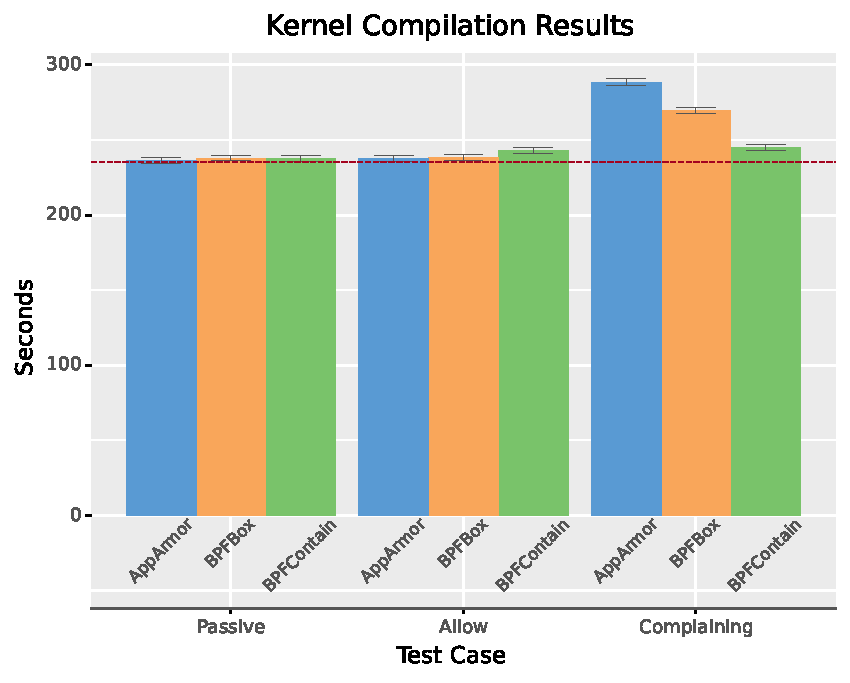
\includegraphics[width=0.6\linewidth]{results/graphs/Kernel-Compilation.pdf}
  \caption[Results of the kernel compilation benchmark]{
    Results of the kernel compilation benchmark.
    The error bars show standard deviation and the red line shows the base measurement.
    Lower times are better.
  }\label{fig:phoronix-kernel}
\end{figure}

\begin{figure}[htp]
  \centering
  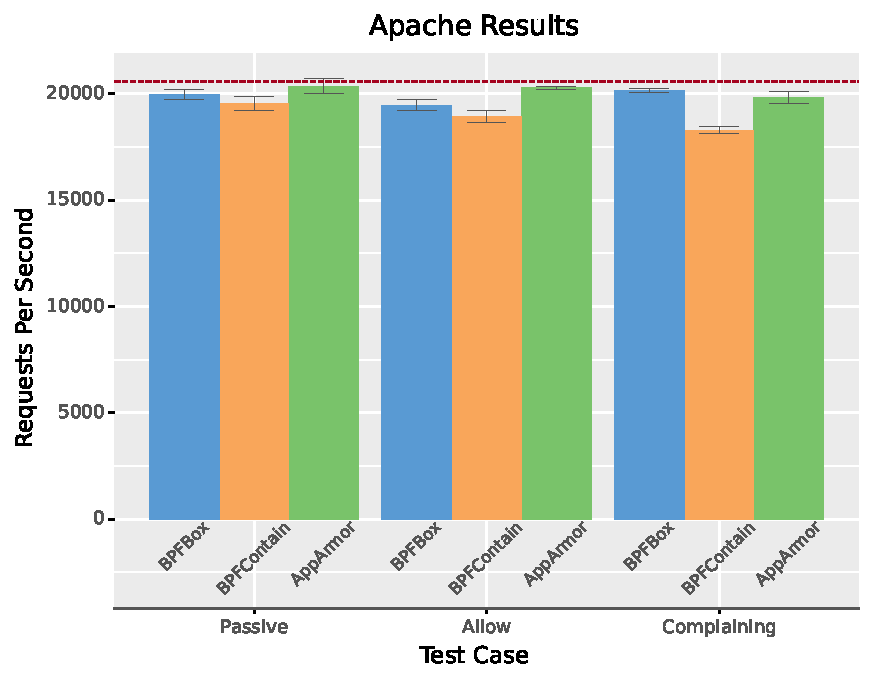
\includegraphics[width=0.6\linewidth]{results/graphs/Apache.pdf}
  \caption[Results of the Apache web server benchmark]{
    Results of the Apache web server benchmark.
    The error bars show standard deviation and the red line shows the base measurement.
    Higher requests per second are better.
  }\label{fig:phoronix-apache}
\end{figure}


\subsubsection{Apache Web Server Results}

The Apache web server benchmark (\Cref{tab:phoronix-apache} and
\Cref{fig:phoronix-apache}) indicates that, while \bpfbox{} and \bpfcontain{} do exhibit
a higher performance overhead than AppArmor, this overhead is still within an acceptable
range at around $11\%$ in the worst case for \bpfcontain{}. This overhead should still be
quite acceptable in practice, and can be improved through further optimizations in
\bpfcontain{}'s enforcement engine, which is still in the prototype phase. The results
from the \textbf{Complaining} case appear to indicate a slight performance improvement for
\bpfbox{} over AppArmor; this is likely due to variance in the measurements rather than
a true performance improvement, as the difference between the two systems falls within the
margin of error.

It is worth noting that, due to an intentional \gls{abi} breakage in the upstream AppArmor
module, AppArmor currently does not enforce any network policy on a stock Linux
kernel~\cite{apparmor_net1, apparmor_net2}. These results were confirmed experimentally
when inspecting the AppArmor logs for the Apache \textbf{Complaining}  test case. This
means that the performance results for AppArmor in the Apache test were at least
significantly biased in favour of AppArmor.  Future experimentation is required with
a patched version of the Linux kernel to determine AppArmor's real overhead in this test
case. We hypothesize that AppArmor's true overhead will more closely match
\bpfcontain{}'s.





\subsection{Discussion of Performance Results}\label{ss:eval-performance-discussion}

The results of the benchmarking tests show that both \bpfbox{} and \bpfcontain{} incur
acceptable performance overhead in practice. In many cases, overhead is competitive with
AppArmor. In other cases, the performance overhead of \bpfbox{} and \bpfcontain{} is
higher than that of AppArmor, but still within a modest range, such that the slowdown
should be either imperceptible or acceptable in many use cases.  As \bpfbox{}
and \bpfcontain{} are both research prototypes, they have not yet been optimized to the
extent that AppArmor has. This lack of optimization is particularly evident in the results
for \bpfcontain{}, and may account for significant differences in performance in the file
I/O and Apache web server tests.

\begin{table}[ht]
  \centering
  \footnotesize
  \caption[Geometric means of Phoronix benchmarking results]{
    Geometric means of Phoronix benchmarking results, as provided by the Phoronix Test
    Suite. These are indicative of overall performance across all tests. For test case,
    percent change from the base results are also given. Higher values are better.
  }\label{tab:phoronix-geometric}
  \begin{tabular}{llrr}
  \toprule
             &               & Geom. Mean & Overhead (\%)\\
   Test Case & System        &            &              \\
   \midrule
   Base      &               & 6.238          & --- \\
   \cline{1-4}
   Passive   & \bpfbox{}     & 6.007          & 3.70\% \\
             & \bpfcontain{} & 5.951          & 4.60\% \\
             & AppArmor      & 6.158          & 1.28\% \\
   \cline{1-4}
   Allow     & \bpfbox{}     & 5.944          & 4.71\% \\
             & \bpfcontain{} & 5.763          & 7.61\% \\
             & AppArmor      & 6.086          & 2.35\% \\
   \cline{1-4}
   Complaining  & \bpfbox{}     & 5.823          & 6.65\% \\
             & \bpfcontain{} & 5.693          & 8.74\% \\
             & AppArmor      & 4.962          & 20.46\% \\
  \bottomrule
  \end{tabular}
\end{table}

While \bpfbox{} and \bpfcontain{} are not as efficient as AppArmor in the \textbf{Passive}
and \textbf{Allow} test cases, the additional performance overhead comes with an increase
in flexibility and system observability afforded by an \gls{ebpf} implementation as
opposed to a traditional Linux Security Module.  Moreover, \bpfcontain{} extends
\bpfbox{}'s original enforcement model, adding new rule categories and enforcement
defaults. While these enhancements may be the cause of some additional performance
overhead, we hypothesize that the majority of \bpfcontain{}'s performance overhead is due to
sub-optimal memory allocations and data structure access patterns, which can be optimized
in the future.

Despite under-performing in the \textbf{Passive} and \textbf{Allow} cases, both \bpfbox{}
and \bpfcontain{} significantly outperform AppArmor in the \textbf{Complaining} test case,
due to a more efficient event logging mechanism. \Cref{tab:phoronix-geometric} shows the
geometric mean of all tests for each test case, indicating that \bpfbox{} and
\bpfcontain{} exhibit an average performance penalty of under $9\%$ in practice, while
AppArmor can exhibit overheads of up to $20\%$ in the worst case.

Although the results presented in this section indicate a comparative performance with
AppArmor, many other widely-adopted \glspl{lsm} can perform significantly worse than
AppArmor in some cases. For instance, Zhang \etal~\cite{zhang2021_lsm_file_overhead} found
that SELinux, perhaps the most widely-used Linux \gls{mac} implementation, exhibits
significant performance overhead, many times worse than AppArmor in some cases. These
results could indicate that \bpfbox{} and \bpfcontain{} might perform favourably compared
to alternative \glspl{lsm} like SELinux, although further investigation is needed in order
to establish a direct comparison.

\section{Security Analysis}\label{s:eval-security}

We now turn our attention to the security of \bpfbox{} and \bpfcontain. Specifically, we
conduct an informal security analysis on both systems, evaluating how well they are able
to confine an attacker under the threat model presented in \Cref{s:cp-threat-model}. In
particular, we examine the various policy rule categories provided by both \bpfbox{} and
\bpfcontain{} as well as how their respective enforcement engines enforce policy at
runtime. We characterize an adversary's ability to escape confinement based on whether the
adversary is able to violate the security assumptions of \bpfbox{} and \bpfcontain{} under
a policy designed to prevent such violations.



\subsection{Threat Model Revisited}

Recall the threat model presented in \Cref{s:cp-threat-model}. We assume a remote
adversary who is confined by some policy $\mathcal{P}$. The adversary's goal is to escape
confinement by circumventing $\mathcal{P}$, enabling them to access sensitive resources,
interfere or tamper with the system, or perform other unauthorized actions. Our goal is to
confine the adversary, limiting the set of all actions they can perform to some subset of
allowed actions. We express such confinement using the policy $\mathcal{P}$ which defines
rules governing the set of operations some subject $\mathcal{S}_i$ may perform on system
objects $\mathcal{O}_1 \mathellipsis \mathcal{O}_n$. To enforce our confinement policy, we
rely on a \textit{confinement engine} which has been loaded into the kernel's reference
monitor.

Under our threat model, we assign significant capabilities to the adversary. Aside from the
restrictions imposed by our confinement policy, we assume that they have root-level access
to the system, including the ability to load code into the kernel, bypass discretionary
access controls, read or modify any persistent resource, and establish persistent access
to the system. Thus, an attacker that is able to escape or bypass confinement has
effectively compromised the entire system. Further, our enforcement engine must take steps
protect itself, preventing the attacker from simply loading or modifying code in the
kernel, which would result in the ability to tamper with or bypass the enforcement engine.

In the subsections that follow, we consider four broad access categories and describe how
\bpfbox{} and \bpfcontain{}'s confinement policy and enforcement engine prevent attacks
related to these access categories. In some cases, the original \bpfbox{} policy
specification (as presented in this thesis) provided insufficient protection against
specific access patterns. In these instances, we describe how \bpfcontain{} improves upon
the original \bpfbox{} design.

\subsection{Files, Filesystems, and Kernel Interfaces}

Correct mediation of file and filesystem accesses is critical to ensure that an adversary
is confined. Files define the canonical persistent data store in modern \gls{cots}
operating systems, including Linux. Depending on the nature of the file, the information
stored within may be confidential, security sensitive, or otherwise critical to normal
system operation. Attacker modification of persistent files is often the first step in
mounting a Confused Deputy attack~\cite{hardy1988_confused_deputy} for privilege
escalation, along with other classes of attack such as data corruption, information
disclosure, and memory safety attacks.

Under the Unix model, special files and filesystems define an entry point into kernel
interfaces, many of which are security sensitive. For example, character devices expose an
interface into device drivers, while special filesystems like \texttt{sysfs} and
\texttt{securityfs} expose behavioural parameters and export sensitive information such as
the system memory map. Limiting access to these files is of paramount importance, since
unrestricted access could enable an attacker to change the behaviour of the kernel, read
sensitive information, modify global system parameters, or interfere with arbitrary user
processes.

In order to restrict access to files (and special files), our enforcement engine must have
complete mediation over the set of all file operations exposed by the \gls{os} kernel and
our policy language must be expressive enough such that it can express the set of all
allowed operations on a specific filesystem object (e.g.\ an inode).

\subsubsection{\bpfbox{}}

To confine a process's access to the filesystem, \bpfbox{} supports \enquote{file} rules
(c.f.\ \Cref{ss:bpfbox-filesystem-rules}), which take a pathname and corresponding access
vector. This access vector encodes the specific file operations that a process can perform
on the file. Since \bpfbox{} policies are default deny, an adversary running under
a \bpfbox{} confinement policy should be unable to perform an operation $Op_i$ on any file
$F_j$ unless this operation is explicitly covered under a file rule. For the purposes of
confinement, \bpfbox{} treats all files equally, regardless of whether the file is
a special file or belongs to a special filesystem. Thus, any access to any file on the
system is governed by the same set of file rules. The only exception to this is a special
\enquote{proc} rule which enables a policy to define access to per-pid \texttt{procfs}
entries belonging to another process.

To enforce its file policy, the \bpfbox{} enforcement engine instruments \gls{ebpf}
programs on several \gls{lsm} hooks, including inode-based, file-based, and path-based
hooks. Taken together, these hooks provide mediation\footnote{This mediation is complete
insofar as the \gls{lsm} hook placement is correct. While this has not been formally
verified, \gls{lsm} hook placement is the basis for security guarantees of all
\glspl{lsm}.} over the set of all file operations, by instrumenting access at the
\gls{vfs} layer. \bpfbox{} encodes its file policy using an \gls{ebpf} map, taking the
inode and device numbers associated with a file and its filesystem as a key. When
a process requests access to a file, \bpfbox{} computes a key for that file and makes
a query against its policy map. This technique has a natural side effect of eliminating
\gls{toctou} race conditions on a file's pathname, since inodes are resolved at policy
load time.

Despite being able to uniquely identify a file, \bpfbox{}'s inode resolution strategy is
subject to a few fundamental limitations. Since inode's are resolved at policy load time,
\bpfbox{} traces the confined process, granting implicit access to any files that the
process creates during its lifecycle.  An attack against this model would consist of
unlinking and re-creating a file after a policy has been loaded, causing \bpfbox{} to see
it as a different file when enforcing access control. In the worst case, this is
effectively a denial of service against the confined process, since \bpfbox{} enforces
a default-deny policy on unrecognized files. However, this attack would also require the
adversary to be unconfined or to be operating under a confinement policy that permitted
the necessary operations on the file.

\subsubsection{\bpfcontain{}}

Like \bpfbox{}, \bpfcontain{} supports file rules that specify a target pathname and
corresponding access vector. In addition to file rules, \bpfcontain{} also supports
filesystem rules for defining per-filesystem policy. A filesystem rule can be thought of
as a coarser-grained version of a file rule, specifying access at the per-filesystem
rather than the per-file level. In order to ensure mediation over explicit denials,
\bpfcontain{} always prioritizes fine-grained file rules over coarse-grained filesystem
rules. This prevents a policy from inadvertently obviating its own file rules with
a careless filesystem rule.

Due to current limitations of \gls{ebpf}, \bpfcontain{} currently uses the same inode
resolution strategy as \bpfbox{}. The strengths and weaknesses of this technique are the
same as in \bpfbox{}, with no major differences. However, future versions of \bpfcontain{}
may move to runtime path-based resolution, once the kernel offers better support for
string helpers and unbounded loops.

Unlike \bpfbox{}, \bpfcontain{} treats regular files differently from special files and
special filesystems. This improves security, as not only do special files and filesystems
have different semantics from regular files, but they also directly expose interfaces into
(potentially untrusted) kernel code. Rather than resolving special files by inode and
filesystem number, \bpfcontain{} looks at their major and minor number pair. Taken
together, these two numbers always uniquely identify a special file, regardless of when it
was created or whether it exists in multiple places at once. This resolution strategy is
not vulnerable to the same attack as the inode resolution strategy, since the adversary
cannot control a device's major and minor number. However, since modern systems
dynamically allocate device numbers, this could cause inconsistencies between the policy
and the system, potentially resulting in spurious policy decisions on device access. To
fix this problem, a future version of \bpfcontain{} will resolve device numbers using
a pathname at runtime.

Rather than being outright default deny, \bpfcontain{} uses heuristics to determine the
appropriate default policy action on system objects. In the case of regular files,
\bpfcontain{} checks to see whether the filesystem superblock is a part of the container's
user namespace (provided that namespace is not the global namespace). If it is, the
filesystem was mounted within the context of the container, and so it is safe to allow
access. Otherwise, access is denied. Since special files and filesystems can be
significantly more dangerous, \bpfcontain{} assumes a default-deny policy instead. This
strategy allows \bpfcontain{} to (under certain conditions) relax requirements on policy
authors without sacrificing security.

\subsection{POSIX Capabilities and Privileged System Calls}

Under Linux, POSIX capabilities~\cite{posix_capabilities} define a process' ability to
override discretionary access controls and access certain privileged kernel interfaces.
Although these cannot be used to override mandatory access controls (such as those
enforced by \bpfbox{} and \bpfcontain{}), they still provide a means of limiting the power
of the root user. This becomes particularly evident in the case of privileged kernel
interfaces which can affect global system state or enable an attacker to load untrusted
code into the kernel.

\subsubsection{\bpfbox{}}

The \bpfbox{} prototype presented in this thesis does not directly interact with POSIX
capabilities in any way. Instead, \bpfbox{} denies access to system resources using its
\gls{lsm} hooks directly. To prevent the adversary from interfering with \bpfbox{}'s
\gls{ebpf} programs or maps, \bpfbox{} always denies the \texttt{bpf(2)} system call from
a confined process, as well as any system calls that could load code into the kernel
(e.g.\ load a kernel module).

The current version of \bpfbox{} does not perform any access validation on mounting
filesystems, which could potentially allow an attacker to modify the global filesystem
hierarchy or interfere with the operation of other processes. This weakness was fixed in
\bpfcontain{} with the additional instrumentation of the \texttt{sb\_mount} \gls{lsm}
hook.

\subsubsection{\bpfcontain{}}

Unlike \bpfbox{}, \bpfcontain{} provisions policy authors with a way to limit the POSIX
capabilities that a container can access. This is done using a \enquote{capability} rule,
which takes a list of capabilities. When a containerized process wishes to use
a capability, it must already possess the capability, pass existing checks in the kernel,
and pass \bpfcontain{}'s capability rule checks. This improves security by introducing an
additional layer of control over a process' bounding capability set.

Like \bpfbox{}, \bpfcontain{} places restrictions on the \texttt{bpf(2)} system call,
ensuring that a confined process can never interfere with its \gls{ebpf} programs or maps.
This ensures that an adversary cannot trivially escape confinement by passing the
enforcement engine. Further, \bpfcontain{} instruments the \texttt{locked\_down} \gls{lsm}
hook which mediates kernel features that could potentially enable arbitrary code execution
in kernelspace.  We explicitly deny any such action, ensuring that a confined process
cannot directly interfere with \bpfcontain{} or other aspects of the kernel.

In addition to limiting \texttt{bpf(2)} and kernel modules, \bpfcontain{} places similar
restrictions on the perf events subsystem (a debugging feature supported by the kernel
that enables tracing the \gls{cpu} and system calls). \bpfcontain{} also blocks operations
that could impact the global system state, such as accessing the kernel keyring, rebooting
the system, modifying system network policy, or changing the system time.

To prevent a confined process from manipulating the layout of the filesystem or subverting
\bpfcontain{}'s default policy at runtime, \bpfcontain{} prohibits a confined process from
mounting or unmounting any filesystems using the \texttt{sb\_mount} \gls{lsm} hook.
\bpfcontain{} also prevents a confined process from changing its namespace by
instrumenting an fentry program on the \texttt{site\_task\_namespaces} kernel function.
This provides improved security over traditional \gls{lsm}-based approaches, as no
\gls{lsm} hook currently guards changing namespaces.

\subsection{Networking}

Access to the kernel's networking stack enables an adversary to connect to remote hosts,
potentially enabling the exfiltration of sensitive data or providing an entry point for
additional attacks. A network socket could also be used by an attacker to bypass
inter-process communication checks (i.e.\ two processes could communicate over the network
instead of using canonical \gls{ipc} mechanisms provided by the kernel). Thus, securing
the kernel's networking stack is critically important for ensuring confinement.


\subsubsection{\bpfbox{}}

\bpfbox{} secures the network stack at the socket layer, defining \enquote{network} rules
that map address families to a set of allowed socket operations. Since \bpfbox{} is
default deny, a policy without any network rules will implicitly cause any socket
operations to be denied by default, thus preventing the process from accessing the network
stack. Using a network operation as a taint rule enables \bpfbox{} to start enforcing
a stricter policy once a process has started communicating with the outside world,
improving security in the case where a remote adversary wants to interact with a process
or exfiltrate sensitive information.

The \bpfbox{} prototype presented in this thesis does not support defining more advanced
network policy at the protocol level (e.g.\ filtering network traffic by \gls{ip} addresses
and port numbers). This means that \bpfbox{} cannot discriminate between network traffic
according to its source and destination, potentially enabling network-based attacks for
software that requires a network connection to function.


\subsubsection{\bpfcontain{}}

Like \bpfbox{}, \bpfcontain{} defines network policy at the socket layer, through its own
\enquote{network} rules. However, \bpfcontain{} greatly simplifies the \bpfbox{} model by
restricting network rules to the IPv4 and IPv6 address families. Other families are either
covered under \gls{ipc} rules (c.f.\ the next subsection) or are outright denied by
default. Future versions of \bpfcontain{} may define additional rules for interacting with
other address families like netlink.

As with \bpfbox{}, \bpfcontain{} does not currently support defining network policy at the
protocol-level. This opens a \bpfcontain{} container up to the same class of network-based
attacks as \bpfbox{}, so long as the container already has access to the networking stack
through its \bpfcontain{} policy. Network firewalls like \texttt{iptables} can be used to
provide additional network security, but future versions of \bpfcontain{} will support
such policy natively, obviating the need to use \texttt{iptables}.

\subsection{\glsentryshort{ipc}}

Inter-process communication mechanisms enable processes to communicate with each other,
sending data back and forth, sending signals to each other, or sharing resources such as
open file descriptors. Without a secure \gls{ipc} policy, an adversary may be able to
trivially escape confinement by establishing a communication channel with an unconfined
process or sharing information or resources between two processes running under
a different confinement policy. Thus, securing \gls{ipc} communication is essential to
ensuring that confinement guarantees hold.

\subsubsection{\bpfbox{}}

\bpfbox{} provisions three rules for \gls{ipc} access: \enquote{ptrace} rules,
\enquote{signal} rules, and \enquote{network} rules using the \texttt{AF\_UNIX} address
family. These rules cover ptrace, signal, and Unix socket access respectively. Ptrace
rules can be used to control whether a confined process can ptrace other processes and
whether another process can ptrace a confined process, providing two-way protection.
Signal rules control the ability for a confined process to send specific categories of
signals to another process. Signals are categorized based on their implications, with
fatal and uncatchable signals belonging to their own category due to their increased
severity. A network rule with the address family of Unix controls a process' ability to interact
with Unix domain sockets. Named pipes are covered under \bpfbox{}'s file policy.

The \bpfbox{} prototype presented in this thesis does not provide a way to control which
process is at the other end of a Unix socket, resulting in potential security
vulnerabilities when a confined process is able to establish a socket connection with an
unconfined process. Another weakness in \bpfbox{}'s current \gls{ipc} policy is that it
does not provision rules for restricting access to System V \gls{ipc} objects.
\bpfcontain{} addresses these shortcomings as explained below.

\subsubsection{\bpfcontain{}}

Rather than defining multiple rule categories for \gls{ipc}, \bpfcontain{} defines
a single \enquote{\gls{ipc}} rule, which takes as an argument the name of another
\bpfcontain{} policy. This rule can be used to grant mutual \gls{ipc} access between two
containers running under a different policy. If either policy does not include an
\gls{ipc} rule granting access to the other, access is denied. This ensures that both
policies mutually agree that they should be able to communicate, eliminating the problem
of an adversary stealthily infiltrating or exfiltrating data into or out of a confined
container.

\gls{ipc} rules under \bpfcontain{} cover all categories of \gls{ipc} under Linux,
including Unix sockets, System V \gls{ipc}, pipes, and signals. The justification for this
is that one \gls{ipc} technique is more or less equivalent to another, and thus allowing
one category of \gls{ipc} but not another does not provide any additional security. Due to
\bpfcontain{}'s container-specific default policy, processes within the same container are
allowed to communicate with each other without defining any \gls{ipc} rules. This is
acceptable since we treat the container as a unit of security.

Ptrace access is also covered under \bpfcontain{}'s default policy. A process may ptrace
another if and only if the two processes exist in the same container. Otherwise, access is
denied. Since ptrace is an extremely powerful interface (effectively giving the tracer
total control over the tracee), \bpfcontain{} defines no policy rules to make exceptions
to its default ptrace enforcement.


\section{Summary}\label{s:eval-summary}

In this chapter, we have evaluated the performance and security of the \bpfbox{} and
\bpfcontain{} research prototypes. We conduct a series of benchmarking tests to evaluate
performance in comparison to the base system and AppArmor, a widely-used \gls{lsm} that
has been upstreamed in the Linux kernel. We find that \bpfbox{} and \bpfcontain{} exhibit
modest percent overhead over AppArmor in the majority of tests, and that they can
outperform AppArmor under specific circumstances. While \bpfcontain{} introduces
additional performance overhead on top of the original \bpfbox{} design, this comes with
additional flexibility, improved security, and a more nuanced default policy. Since
\bpfbox{} and \bpfcontain{} are kernel agnostic, we can update them without updating the
host kernel, enabling bugs to be fixed like userspace programs. Further, we argue that
\bpfcontain{} can be significantly optimized in the future, enabling future iterations on
the design to perform more competitively with existing \glspl{lsm}.

An informal security analysis reveals that \bpfbox{} and \bpfcontain{} found limitations
in \bpfbox{} that were later addressed in \bpfcontain{}, such as a lack of support for
capability-level policy and limited support for restricting access to \gls{ipc} objects.
\bpfcontain{} resolves the majority of \bpfbox{}'s limitations while simultaneously
simplifying the policy language. While \bpfcontain{} also has limitations with respect to
device-level policy and coarse-grained network policy, these can be addressed in future
work (see \Cref{c:discussion}).



\chapter{Case Studies}\label{c:case-studies}
In this chapter, we examine specific case studies, where we apply \bpfbox{} and
\bpfcontain{} policies to solve realistic problems. We examine how \bpfbox{} and
\bpfcontain{} can be used to confine a webserver and database and how they can implement
the default Docker confinement policy.  We also discuss how future extensions to
\bpfcontain{} could enable it to confine an untrusted container with a minimal policy file.
To offer a basis for comparison, we contrast presented policies with some available
equivalents and discuss how the semantics of the policy language and enforcement engine
can impact the resulting policy file.



\section{Confining a Web Server and Database}

We first examine a practical use case: confining a simple web server and database
deployment. In particular, we focus on the Apache httpd web server and the MySQL database
management system. These two pieces of software are often used together (e.g.\ as part of
the LAMP stack~\cite{lamp}) and provide a good example of how we can define specific
policy exceptions to allow two processes or containers to communicate with each other and
with the outside world. In this example, we assume that httpd and mysqld communicate with
each other using a shared Unix domain socket created by mysqld. We synthesize policies
through a combination of running the programs under \texttt{strace}, finding library
dependencies with \texttt{ldd}, and running the programs under \bpfcontain{}'s complaining
mode. We use the output of these tools along with \bpfcontain{}'s log output to write
the security policies by hand.

\subsubsection{\bpfbox{}}

In \bpfbox{}, we define two profiles: one for httpd, and one for mysqld.
\Cref{lst:bpfbox-apache} depicts the httpd policy while \Cref{lst:bpfbox-mysql} depicts
the mysqld policy. These policies are simplified examples but provide a representative
idea of what it's like to confine a complex application down to its basest functionality.

The httpd policy (\Cref{lst:bpfbox-apache}) defines allow and taint rules for three
categories of socket access: \texttt{inet}, \texttt{inet6}, and \texttt{unix}. These
categories cover IPv4 and IPv6 network access as well as \gls{ipc} over a Unix domain
socket. This Unix domain socket is what httpd will use to communicate with the database.
By defining these network rules as both allow and taint, we indicate that default-deny
enforcement should begin only \textit{after} the Apache daemon has begun interacting with
the outside world. Using this technique, the \bpfbox{} policy may be greatly simplified by
eliminating the need to define any policy corresponding to the setup phase of httpd.

The bulk of the \bpfbox{} policy is made up of filesystem rules, enabling access to
a variety of configuration files that httpd needs to read at runtime, a few informational
files exposed by the kernel under procfs, shared libraries that may be loaded at runtime,
the mysqld Unix socket, and the directory that httpd will use to serve web content. We
also define a rule allowing httpd to run suexec, a helper application used to launch
\gls{cgi} scripts.  We indicate that launching suexec should untaint the process and
transition to a suexec profile.  This profile would then define the access control policy
for suexec (e.g.\ which scripts it is allowed to run).

\begin{lstlisting}[language=bpfbox, gobble=4, float=false, caption={[A \bpfbox{} policy for Apache httpd]
  A \bpfbox{} policy for Apache httpd.
}, label={lst:bpfbox-apache}]
    #![profile "/bin/httpd"]

    /* Allow IP and Unix socket operations, and taint when
     * sending or receiving */
    #[allow] {
      net(inet, any)
      net(inet6, any)
      net(unix, any)
    }
    #[taint] {
      net(inet, send|recv)
      net(inet6, send|recv)
      net(unix, send|recv)
    }

    #[allow] {
      /* Allows kill(2) to check for process existence
       * and to send fatal signals */
      signal("/bin/httpd", check|fatal)

      /* Write to logs */
      fs("/var/log/httpd/*log", getattr|read|append)
      fs("/var/log/httpd", getattr|read|write)

      /* Create PID file */
      fs("/run/httpd/", write)
      /* Delete or modify an existing PID file if necessary */
      fs("/run/httpd/httpd.pid", getattr|rm|write)

      /* Serve files from /srv/html/ and all subdirectories */
      fs("/srv", read|getattr)
      fs("/srv/html", read|getattr)
      fs("/srv/html/**", read|getattr)

      /* Access to mysqld socket */
      fs("/run/mysqld", getattr|read)
      fs("/run/mysqld/mysqld.sock", getattr|read|write)

      /* Read configuration */
      fs("/usr/share/httpd/**", read|getattr)
      fs("/etc/httpd/", getattr)
      fs("/etc/httpd/conf/**", read|getattr)
      fs("/usr/share/zoneinfo/**", read|getattr)

      /* Read hostname information */
      fs("/etc/resolv.conf", read|getattr)
      fs("/etc/host*", read|getattr)

      /* Read-only access to required kernel info */
      fs("/proc/sys/kernel/random/boot_id", read)
      fs("/proc/sys/kernel/ngroups_max", read)

      /* Shared libraries loaded at runtime */
      fs("/usr/lib/httpd/modules/*.so", getattr|read|exec)
      fs("/usr/lib/libnss*.so.*", getattr|read|exec)
      fs("/usr/lib/libgcc_s.so.*", getattr|read|exec)
    }

    /* Transition to a separate suexec policy */
    #[transition] {
      fs("/usr/bin/suexec", getattr|read|exec)
    }
\end{lstlisting}

The \bpfbox{} policy for mysqld works in much the same way as the policy for httpd. Major
differences include disabling all socket access except to Unix domain sockets. This
ensures that the database is not exposed to the outside world but still enables is to
communicate with httpd over its Unix socket. Like with httpd, we define specific rules
enabling mysqld to read important configuration files, log events, create and modify its
\gls{pid} file and Unix socket, and load some shared libraries at runtime. The entire
setup phase for mysqld occurs while the process is untainted, thus allowing us to
eliminate rules for any shared libraries loaded before the process becomes tainted.

\begin{lstlisting}[language=bpfbox, gobble=4, float=false, caption={[A \bpfbox{} policy for MySQL]
  A \bpfbox{} policy for MySQL.
}, label={lst:bpfbox-mysql}]
    #![profile "/bin/mysqld"]

    /* Allow Unix socket operations, and taint when
     * sending or receiving. Also allow creating and
     * binding inet and inet6 sockets (necessary to
     * pass assertion checks) */
    #[allow] {
      net(unix, any)
      net(inet, create|bind)
      net(inet6, create|bind)
    }
    #[taint]
    net(unix, send|recv)

    #[allow] {
      /* Allows kill(2) to check for process existence
       * and to send fatal signals */
      signal("/bin/mysqld", check|fatal)

      /* /dev/null and /dev/urandom */
      fs("/dev/null", getattr|read|write)
      fs("/dev/urandom", getattr|read)

      /* Write to logs */
      fs("/var/log/mysqld/*log", getattr|read|append)
      fs("/var/log/mysqld", getattr|read|write)

      /* Access to /var/lib/mysql */
      fs("/var/lib/mysql", read|write|getattr)
      fs("/var/lib/mysql/**", read|write|getattr|rm)

      /* Create PID file and socket */
      fs("/run/mysqld", getattr|read|write)
      fs("/run/mysqld/**", getattr|read|write|rm)

      /* Read configuration */
      fs("/etc/mysql", read|getattr)
      fs("/etc/mysql/**", read|getattr)
      fs("/usr/share/zoneinfo", read|getattr)
      fs("/usr/share/zoneinfo/**", read|getattr)

      /* Shared libraries loaded at runtime */
      fs("/var/lib/mysql/plugin/*.so", getattr|read|exec)
      fs("/usr/lib/libnss_files-*.*.so", getattr|read|exec)
    }
\end{lstlisting}

\subsubsection{\bpfcontain{}}

In \bpfcontain{} we once again define a policy for httpd and a policy for mysqld.  These
policies are depicted in \Cref{lst:bpfcontain-apache} and \Cref{lst:bpfcontain-mysql}
respectively. These policies are largely similar to the \bpfbox{} policies, with a few
minor differences that can be attributed to \bpfcontain{}'s nuanced policy defaults and
its updated policy language.

Like \bpfbox{}, the majority of the \bpfcontain{} httpd policy
(\Cref{lst:bpfcontain-apache}) focuses on specifying filesystem access for httpd. Since
\bpfcontain{} also supports tainting semantics, we leverage these to eliminate the need to
define rules for operations preceding the taint. Specifically, we taint container once it
has performed any networking operations or any \gls{ipc} with mysqld. Unlike \bpfbox{},
however, \bpfcontain{} does not support untainting a process. This is a natural extension
of the fact that \bpfcontain{} deals in container semantics rather than process-level
confinement\,---\,it does not make sense to untaint and transition profiles in the context
of a container, since a single security policy applies to the entire container. This
means that we must still specify access to shared libraries that will be loaded by suexec
(along with whatever applications suexec will run, such as Python).

Aside from the aforementioned differences, the per-file policy is more or less the same as
\bpfbox{}. To enable \gls{ipc} between the httpd and mysql, we define an \gls{ipc} allow
rule that lists the mysqld policy. We also enable socket networking using a network allow
rule and enable signalling of existing instances of httpd with a signal rule. Finally, we
use a capability rule to grant access to the \texttt{CAP\_NET\_BIND\_SERVICE} capability,
allowing httpd to bind to privileged ports. Since \bpfbox{} does not support capability
rules, there is no equivalent to this rule in the \bpfbox{} policy, meaning that POSIX
capabilities would effectively be unrestricted.

\begin{lstlisting}[language=yaml, gobble=2, float=false, caption={[A \bpfcontain{} policy for Apache httpd]
  A \bpfcontain{} policy for Apache httpd.
}, label={lst:bpfcontain-apache}]
  name: httpd
  defaultTaint: false

  allow:
    # /dev/urandom, /dev/random, /dev/null
    - dev: random
    - dev: null

    # Access to log files
    - file: {pathname: /var/log/httpd, access: rw}
    - file: {pathname: /var/log/httpd/*log, access: ra}

    # Create pidfile, delete or modify an existing pid file if necessary
    - file: {pathname: /run/httpd, access: rw}
    - file: {pathname: /run/httpd/**/*, access: rwd}

    # Read configuration
    - file: {pathname: /usr/share/httpd/**/*, access: r}
    - file: {pathname: /etc/httpd, access: r}
    - file: {pathname: /etc/httpd/conf/**/*, access: r}
    - file: {pathname: /usr/share/zoneinfo/**/*, access: r}

    # Serve files
    - file: {pathname: /srv, access: r}
    - file: {pathname: /srv/html, access: r}
    - file: {pathname: /srv/html/**, access: r}

    # Read hostname information
    - file: {pathname: /etc/resolv.conf, access: r}
    - file: {pathname: /etc/host*, access: r}

    # Shared libraries loaded at runtime
    - file: {pathname: /usr/lib/httpd/modules/*.so, access: mr}
    - file: {pathname: /usr/lib/libnss*.so.*, access: mr}
    - file: {pathname: /usr/lib/libgcc_s.so.*, access: mr}

    # Execute suexec and python
    - file: {pathname: /usr/bin/suexec, access: rx}
    - file: {pathname: /usr/bin/python, access: rx}

    # Shared libraries required for suexec and python
    # This is unfortunately required since BPFContain currently
    # has no notion of untainting like BPFBox
    - file: {pathname: /usr/lib/libpython*.so.*, access: mr}
    - file: {pathname: /usr/lib/libc.so.*, access: mr}
    - file: {pathname: /usr/lib/libpthread.so.*, access: mr}
    - file: {pathname: /usr/lib/libdl.so.*, access: mr}
    - file: {pathname: /usr/lib/libutil.so.*, access: mr}
    - file: {pathname: /usr/lib/libm.so.*, access: mr}
    - file: {pathname: /usr/lib64/ld-linux-x86-64.so.*, access: mr}

    # Allow ipc with mysql
    - ipc: mysqld

    # Allow sending signals to existing httpd instances
    - ipc: httpd

    # Bind to privileged ports, change uid and gid
    - capability: [netbindservice, setuid, setgid]

    # Use networking
    - net: [server, send, recv]

  taint:
    # Taint when performing any ipc or networking
    - net: [send, recv]
    - ipc: mysqld
\end{lstlisting}

The mysqld policy for \bpfcontain{} (\Cref{lst:bpfcontain-mysql}) also shares many
similarities with the \bpfbox{} version.  In particular, we define equivalent file access
rules to enable the mysqld to access all of the files it requires for normal operation. We
define an \gls{ipc} rule, granting mutual \gls{ipc} access to the httpd policy, and
enabling the two to communicate with each other. We taint the container once it has
performed any \gls{ipc} with httpd. We enable the creation of new network sockets
in order to pass assertion checks, but otherwise explicitly deny any network access.

\begin{lstlisting}[language=yaml, gobble=4, float=false, caption={[A \bpfcontain{} policy for MySQL]
  A \bpfcontain{} policy for MySQL.
}, label={lst:bpfcontain-mysql}]
    name: mysqld
    defaultTaint: false

    allow:
      # Access to log files
      - file: {pathname: /var/log/mysqld, access: rw}
      - file: {pathname: /var/log/mysqld/*log, access: ra}

      # Access to /var/lib/mysql
      - file: {pathname: /var/lib/mysql, access: rw}
      - file: {pathname: /var/lib/mysql/**/*, access: rwd}

      # Create pidfile and socket
      - file: {pathname: /run/mysqld, access: rw}
      - file: {pathname: /run/mysqld/**/*, access: rwd}

      # Read configuration
      - file: {pathname: /etc/mysql, access: r}
      - file: {pathname: /etc/mysql/**/*, access: r}
      - file: {pathname: /usr/share/zoneinfo, access: r}
      - file: {pathname: /usr/share/zoneinfo/**/*, access: r}

      # Shared libraries loaded at runtime
      - file: {pathname: /var/lib/mysql/plugin/*.so, access: mr}
      - file: {pathname: /usr/lib/libnss_files-*.*.so, access: mr}

      # Allow ipc with httpd
      - ipc: httpd

      # Allow sending signals to existing mysqld instances
      - ipc: mysqld

      # Allow mysqld to create a new network socket
      # (Necessary to pass assertions)
      - net: server

    taint:
      # Taint when performing ipc with httpd
      - ipc: httpd
      # Taint when sending or receiving any network traffic
      - net: [send, recv]

    deny:
      # Explicitly deny sending or receiving any network traffic
      - net: [send, recv]
\end{lstlisting}

\subsubsection{Simplifying the \bpfcontain{} Example}

Once \bpfcontain{} has been fully integrated with Docker support, it may become possible
to greatly simplify the above policy examples, leveraging default filesystem policy to
grant access to all of the required files, without the need to explicitly specify rules
for each file. We leverage a shared \texttt{/tmp} filesystem, mounted on the host, to
allow both mysqld and httpd to access the same Unix socket. The result is an extremely
simple policy that can express all the required interfaces in just a few lines.
\Cref{lst:bpfcontain-httpd-next} and \Cref{lst:bpfcontain-mysqld-next} give example
policies for httpd and mysqld respectively.

\begin{lstlisting}[language=yaml, gobble=4, float=false, caption={[A simplified \bpfcontain{} policy for Apache httpd]
  A simplified \bpfcontain{} policy for Apache httpd running in a Docker container,
  leveraging future support for automatic filesystem policy.
}, label={lst:bpfcontain-httpd-next}]
    name: httpd-container
    defaultTaint: true

    allow:
      # Grant access to global /tmp filesystem, mounted as a Docker volume
      # This is where the mysqld Unix socket will go
      - fs: {pathname: /tmp, access: r}
      # /dev/urandom, /dev/random, /dev/null
      - dev: random
      - dev: null
      # Allow network access
      - net: [server, send, recv]
      # Allow ipc access with mysqld
      - ipc: mysqld-container
      # Bind to privileged ports, change uid and gid
      - capability: [netbindservice, setuid, setgid]
\end{lstlisting}

\begin{lstlisting}[language=yaml, gobble=4, float=false, caption={[A simplified \bpfcontain{} policy for MySQL]
  A simplified \bpfcontain{} policy for MySQL running in a Docker container, leveraging
  future support for automatic filesystem policy.
}, label={lst:bpfcontain-mysqld-next}]
    name: mysqld-container
    defaultTaint: true

    allow:
      # Grant access to global /tmp filesystem, mounted as a Docker volume
      # This is where the mysqld Unix socket will go
      - fs: {pathname: /tmp, access: rw}
      # Allow mysqld to create a new network socket
      # (Necessary to pass assertions)
      - net: server
      # Allow ipc access with httpd
      - ipc: httpd-container
    deny:
      # Explicitly deny sending or receiving any network traffic
      - net: [send, recv]
\end{lstlisting}


\section{The Default Docker Policy}

Docker~\cite{docker_security} applies a coarse-grained default confinement policy to all
containers using a combination of Linux confinement primitives. On supported
systems\footnote{Recall that not all Linux distributions support AppArmor or Seccomp-bpf
to begin with. In such cases, Docker simply discards its default confinement policy
altogether.}, this includes a default AppArmor policy template~\cite{docker_apparmor,
docker_default_apparmor}, a default Seccomp-bpf profile, and a set of POSIX capabilities
which are dropped at runtime~\cite{docker_security}.

Docker's policy defaults are highly coarse grained, with an emphasis on practical security
while ensuring that the vast majority of container configurations will \enquote{just
work,} out of the box. This affords a practical opportunity to examine how \bpfbox{} and
\bpfcontain{} policies compare with the default Docker policy. \Cref{tab:docker-default}
summarizes the key aspects of Docker's confinement policy, highlighting default access
levels enforced by various Linux confinement primitives. \Cref{lst:docker-default} depicts
Docker's default AppArmor template, taken directly from the Docker sources on
GitHub~\cite{docker_default_apparmor}.

\begin{table}[htpb]
  \centering
  \caption[The default Docker confinement policy]{
    A summary of Docker's default confinement policy~\cite{docker_security,
    docker_apparmor, docker_default_apparmor}. Policy is enforced using a number of Linux
    confinement primitives, including AppArmor, Seccomp-bpf, and dropped POSIX
    capabilities at runtime. Docker generates and loads AppArmor policy at container
    runtime using a pre-determined, coarse-grained AppArmor template file
    (c.f.\ \Cref{lst:docker-default}).
  }\label{tab:docker-default}
  \footnotesize
  \begin{tabular}{lp{2in}p{1.6in}}
  \toprule
  Access Category & Default & Docker Implementation \\
  \midrule
  Files & Allow access to all files except specific procfs and sysfs entries. & AppArmor Template \\
  Filesystem Mounts & Deny all filesystem mounts. & AppArmor Template \\
  POSIX Capabilities & All capabilities enabled in AppArmor.  Drop specific capabilities at runtime. & AppArmor Template and Dropped Capabilities \\
  Ptrace & Allowed within container. & AppArmor Template \\
  Signals & Allowed within container. & AppArmor Template \\
  Network & Allow all network access. & AppArmor Template \\
  \gls{ipc} & Allow all \gls{ipc} access. & AppArmor Template \\
  System Calls & Deny about 60 obsolete/dangerous system calls. & Seccomp-bpf \\
  \bottomrule
  \end{tabular}
\end{table}

\begin{lstlisting}[language=none, gobble=4,
  caption={[Docker's default AppArmor template]
    Docker's default AppArmor template~\cite{docker_default_apparmor}, at the time of
    writing this thesis. Docker uses Go's string templating syntax to modify the AppArmor
    profile according to the current Docker version and container metadata.
  },
  label={lst:docker-default}, float]
    {{range $value := .Imports}}
      {{$value}}
    {{end}}
    profile {{.Name}} flags=(attach_disconnected,mediate_deleted) {
    {{range $value := .InnerImports}}
      {{$value}}
    {{end}}
      network,
      capability,
      file,
      umount,
    {{if ge .Version 208096}}
      # Host (privileged) processes may send signals to container processes.
      signal (receive) peer=unconfined,
      # dockerd may send signals to container processes (for "docker kill").
      signal (receive) peer={{.DaemonProfile}},
      # Container processes may send signals amongst themselves.
      signal (send,receive) peer={{.Name}},
    {{end}}
     # deny write for all files directly in /proc (not in a subdir)
      deny @{PROC}/* w,
      # deny write to files not in /proc/<number>/** or /proc/sys/**
      deny @{PROC}/{[^1-9],[^1-9][^0-9],
        [^1-9s][^0-9y][^0-9s],[^1-9][^0-9][^0-9][^0-9]*}/** w,
      # deny /proc/sys except /proc/sys/k* (effectively /proc/sys/kernel)
      deny @{PROC}/sys/[^k]** w,
      # deny everything except shm* in /proc/sys/kernel/
      deny @{PROC}/sys/kernel/{?,??,[^s][^h][^m]**} w,
      deny @{PROC}/sysrq-trigger rwklx,
      deny @{PROC}/kcore rwklx,
      deny mount,
      deny /sys/[^f]*/** wklx,
      deny /sys/f[^s]*/** wklx,
      deny /sys/fs/[^c]*/** wklx,
      deny /sys/fs/c[^g]*/** wklx,
      deny /sys/fs/cg[^r]*/** wklx,
      deny /sys/firmware/** rwklx,
      deny /sys/kernel/security/** rwklx,
    {{if ge .Version 208095}}
      # suppress ptrace denials when using 'docker ps' or using 'ps' inside a container
      ptrace (trace,read,tracedby,readby) peer={{.Name}},
    {{end}}
    }
\end{lstlisting}

\subsubsection{\bpfbox{}}

We begin by examining a mostly equivalent policy in \bpfbox{}, given in
\Cref{lst:bpfbox-docker-default}.  Re-implementing Docker's default confinement policy in
\bpfbox{} is surprisingly challenging. \bpfbox{} is not designed to implement
coarse-grained confinement policy, and so specifying things like global access to all
files is impossible. We compromise by granting recursive access to all files within
a given filesystem, repeating the process for each filesystem as required. This is
\textit{not} the intended use case for \bpfbox{} file rules, but it is required to match
the over-permissive filesystem access provisioned by Docker. Aside from
filesystem-specific policy, most of Docker's default policy can be implemented relatively
easily and cleanly in \bpfbox{}'s policy language.

\begin{lstlisting}[language=bpfbox, gobble=4,
  caption={[Implementing the default Docker policy in \bpfbox{}]
    Implementing the default Docker policy in \bpfbox{}.
},
  label={lst:bpfbox-docker-default}]
    #![profile "/path/to/init/program"]

    #[allow] {
      /* Allow essentially global access to a filesystem */
      fs("/path/to/filesystem/**", read|write|setattr|getattr|rm|link|ioctl)
      /* Repeat for others... */

      /* Allow access to /proc/sys/kernel/shm* */
      fs("/proc/sys/kernel/shm*", read|write|setattr|getattr)

      /* Sensible default access for procfs per-pid entries */
      proc(self, read|write)
      proc(child, read|write)
    }

    #[allow]
    #[taint]
    {
      /* Access to network families */
      net(inet, any)
      net(inet6, any)
      net(unix, any)

      /* Ptrace child processes */
      ptrace(child, read|write|attach)

      /* Send sigchld up to parent processes, any signal to children */
      signal(parent, sigchld)
      signal(child, any)
    }

    #[transition]
    #[untaint]
    {
      /* Allow execve calls to allowed executables,
       * tainting and transitioning profiles when doing so */
      fs("/path/to/allowed/executable", read|exec)
      /* Repeat for others... */
    }
\end{lstlisting}

Like Docker's AppArmor policy, our \bpfbox{} policy enables access to per-pid entries in
procfs and uses \bpfbox{}'s default-deny enforcement to restrict all others. Similar logic
applies to the \texttt{/proc/sys/kernel/shm*} entries under procfs. We also grant full
networking stack access, ptrace access for child processes, and full signal access for
child processes running under the container. Since these operations have the potential to
introduce vulnerabilities from outside sources, we mark them as tainting the corresponding
process. Leveraging taintedness, the \bpfbox{} policy eliminates the need to specify
access to shared library dependencies and other artifacts of the C runtime.

For more complex container deployments that include more than a single binary, the
\bpfbox{} policy may need to specify access to alternative executables under the
container.  We do so using an individual file rule for each executable, optionally
specifying that the process should untaint itself and/or transition to a new profile.
Notably, the version of \bpfbox{} presented in this thesis does \textit{not} include
capability-level policy, and so it is not included here\footnote{\bpfcontain{} later
rectified this gap in \bpfbox{}'s policy language.}. However, the default Docker
confinement policy does not implement capability-level filtering anyway, instead relying
on dropped capabilities at runtime.

Although the \bpfbox{} policy depicted in \Cref{lst:bpfbox-docker-default} does not fully
map to the precise Docker default policy, it gets very close in most respects, aside from
filesystem policy. Under \bpfbox{}, filesystem policy is necessarily finer-grained, as it
does not support the ability to specify coarse-grained access to all files on the system.
Despite these challenges, the end result is a functional (and, in some aspects, more
secure) alternative to the default Docker policy.

\subsubsection{\bpfcontain{}}

Having examined how \bpfbox{} can be used to implement an approximate version of Docker's
default confinement policy, we now turn our attention to \bpfcontain{}.
\Cref{lst:bpfcontain-docker-default} shows the full \bpfcontain{} policy. Note that many
aspects of Docker's default policy are covered by \bpfcontain{}'s default
container-boundary enforcement. Using this to its advantage, the \bpfcontain{} policy is
significantly simpler than both the AppArmor and \bpfbox{} versions while maintaining the
same level of expressiveness.

\begin{lstlisting}[language=yaml, gobble=4,
  caption={[Implementing the default Docker policy in \bpfcontain{}]
    Implementing the default Docker policy in \bpfcontain{}.
},
  label={lst:bpfcontain-docker-default}]
    name: default-docker
    defaultTaint: true

    allow:
      # Grant access to the entire root filesystem
      - fs: {pathname: /, access: any}
      # Grant access to tempfs
      - fs: {pathname: /tmp, access: any}
      # Grant read/write access to /proc/sys/kernel/shm*
      - file: {pathname: /proc/sys/kernel/shm*, access: rw}

      # Grant access to the terminal, /dev/null, /dev/random, and /dev/urandom
      - device: terminal
      - device: null
      - device: random

      # Grant access to the entire networking stack
      - net: any

      # Enable Docker default capabilities
      # All other capabilities are denied
      - capability:
        - chown
        - dacoverride
        - fsetid
        - fowner
        - mknod
        - netraw
        - setgid
        - setuid
        - setfcap
        - setpcap
        - netbindservice
        - syschroot
        - kill
        - auditwrite
\end{lstlisting}

Compared with \bpfbox{}, the \bpfcontain{} version of Docker's default policy is
significantly simpler and fits more cleanly with Docker's AppArmor policy. This
improvement is a direct result of a number of critical differences between \bpfbox{} and
\bpfcontain{}. Whereas \bpfbox{} was designed for fine grained process-level confinement,
\bpfcontain{} was directly designed with containers in mind. Since \bpfcontain{} policies
are designed to be container specific, they are far more appropriate for a use case
centered around the confinement of containers. In particular, \bpfcontain{} incorporates
container semantics into its default policy enforcement, greatly simplifying the resulting
policy.  Further, changes to \bpfcontain{}'s policy language, including the introduction
of a coarser-grained filesystem rule and capability rules enables the resulting policy to
more closely match the original Docker AppArmor policy.

To match Docker's default allow policy on filesystem access, the \bpfcontain{} policy
includes a rule to enable any file operation on files within the root filesystem and
tempfs.  As with \bpfbox{}, the point here is to match Docker's default policy without
considering the security implications of granting full access to the entire root
filesystem. We include another rule to enable similar access on the temporary filesystem.
Despite the coarse granularity of these filesystem rules, \bpfcontain{} maintains
a critical advantage over \bpfbox{} and the original Docker policy. Due to its
container-specific policy defaults, we can achieve Docker's fine-grained protection over
procfs and sysfs without the need to specify it in the security policy.

As with the procfs and sysfs policy, \bpfcontain{} also includes sensible defaults for
\gls{ipc} and ptrace access. In particular, processes running within the same container
are free to perform \gls{ipc} with one another and ptrace one another, so long as the
basic Unix access rights are satisfied (e.g.\ the process possesses CAP\_PTRACE or is the
direct ancestor of the tracee). In the case of signals and ptrace, these defaults directly
match the Docker policy (c.f.\ \Cref{tab:docker-default}).  In other cases, these defaults
are more secure than the Docker policy, while permits all other forms of \gls{ipc}
regardless of container membership.

To prevent a container from escaping confinement or interfering with the host,
\bpfcontain{} prohibits the container from mounting filesystems, loading kernel modules,
using \gls{ebpf}, changing the system time, rebooting the system, or performing a number
of other privileged operations. These defaults also match or exceed Docker's default
policy, and thus may also be omitted from the \bpfcontain{} policy.

While many aspects of \bpfcontain{}'s default enforcement closely match the default Docker
policy, \bpfcontain{}'s defaults remain strictly less permissive. For instance, the
default Docker policy mandates that \texttt{/proc/sys/kernel/shm*} be accessible to
containers, but \bpfcontain{} denies access to all procfs entries that do not belong to
a container process. We define an exception to \bpfcontain{}'s default procfs policy by
adding an explicit allow rule on this pathname. Similarly, \bpfcontain{}'s default policy
forbids network access by default, and so we must explicitly grant the container
permission to use the networking stack. Unlike Docker, \bpfcontain{} prohibits the use of
any POSIX capability that is not directly specified in the policy file. Thus, we include
an additional allow rule that mirrors the set of capabilities dropped by Docker at
runtime.

The resulting \bpfcontain{} policy implements a strict superset of Docker's default
confinement policy, despite being significantly simpler, and more centralized.  Since
\bpfcontain{} directly models the relationship between containerized processes and their
resources, we can achieve significant portions of Docker's default policy for free. In
many cases, this default enforcement is actually finer grained than the Docker defaults.
In order to achieve the same coarse granularity as the Docker policy, we adjust the
\bpfcontain{} policy by incorporating a few additional allow rules, granting access to
specific filesystems, the networking stack, and POSIX capabilities.

\section{Confining an Untrusted Container}

We now examine perhaps the most obvious and practical use case for \bpfcontain{}:
confining an untrusted container. For instance, consider a new container image, freshly
downloaded from Docker Hub, to be used during application development or testing.  We
assume that the system administrator does not trust this container image and wishes to
confine the resulting container, preventing it from damaging the rest of the system,
leaking information, or performing other potentially unwanted actions. For this purpose,
we leverage an extremely simple \bpfcontain{} policy (essentially the canonical
\enquote{Hello World} example) and demonstrate how it can be customized to match the
container's specific needs. \Cref{lst:bpfcontain-untrusted} depicts the \bpfcontain{} policy.

Here, we assume that this policy is applied to a future version of \bpfcontain{}
\textit{with} full Docker integration and automatic filesystem policy.
(\Cref{sss:bpfcontain-improving-default} of \Cref{c:bpfcontain} explains how this will be
done.) Without these extensions, the policy author would need to manually grant access to
files underlying the container's overlay filesystem, either using a filesystem allow rule
or per-file allow rules. While this shouldn't add much additional complexity to the
policy, the specific file rules would largely depend on the container's configuration, and
so we omit the details of such a policy here. For a similar reason, we omit the
corresponding \bpfbox{} policy as well, since \bpfbox{} does not deal in container-level
semantics as \bpfcontain{} does.



\begin{lstlisting}[language=yaml, gobble=4,
  caption={[Confining an untrusted container with \bpfcontain{}]
    Confining an untrusted container with \bpfcontain{}.
    Note that this policy requires some extensions on top of the existing \bpfcontain{}
    model, such as instrumenting the Docker container runtime.
  },
  label={lst:bpfcontain-untrusted}, float=false]
    name: untrusted-container
    defaultTaint: true

    allow:
      # Specify full path and access for volume mounts from the host
      - file: {pathname: /path/to/volume/mount, access: rw}
      # Repeat for other volume mounts as required...

      # If the container requires networking
      # We could also define finer-grained access by replacing the "any"
      # keyword with specific socket operations
      - net: any

      # If the container requires any capabilities
      - capability: [dacoverride, dacreadsearch, netbindservice] # etc.

      # Further extensions to the policy as required...
\end{lstlisting}

We define a default-tainted \bpfcontain{} policy called \enquote{untrusted-container}.
Just this policy alone should be enough to confine a simple container. \bpfcontain{}'s
default policy would prohibit network access, the use of any POSIX capabilities, access to
any files outside of the container's overlay filesystem, and any operations that can
impact the system as a whole. This default policy prevents entire classes of attacks,
prohibiting the container from leaking outside information, changing global system
parameters, loading code into the kernel, or forming unauthorized network connections. The
reader is encouraged to revisit \Cref{fig:bpfcontain-enforcement} on page
\pageref{fig:bpfcontain-enforcement} of \Cref{c:bpfcontain} for a depiction of how
\bpfcontain{}'s default enforcement works.

While the \bpfcontain{} default policy should be sufficient for simple use cases, more
advanced container images may require some slight modification, introducing a few allow
rules to define exceptions in \bpfcontain{}'s protection boundary. For instance, suppose
the container image requires a docker volume to be mounted at runtime. To support this use
case, we define a file rule specifying the system path to the volume mount and the
corresponding access pattern, such as \texttt{rw} for read and write access. All other
accesses to the host filesystem remain denied. If the container requires access to the
networking stack, we similarly define a net rule.  Capability rules can be used to allow
the container to use a selected subset of POSIX capabilities, assuming it already
possesses these capabilities at runtime. For example, we may wish to grant the container
the \texttt{DAC\_OVERRIDE} and \texttt{DAC\_READ\_SEARCH} capabilities to allow it to
interact with the Docker volume we specified earlier, or the \texttt{NET\_BIND\_SERVICE}
capability to allow it to bind to privileged ports.




\section{Summary}

This chapter has presented and compared \bpfbox{} and \bpfcontain{} policies for various
use cases. In particular, we examine how \bpfbox{} and \bpfcontain{} can confine a simple
web server and database deployment,  how each system can be used to implement a policy
resembling the Docker default policy, and how a future version of \bpfcontain{} can be
used to confine an untrusted container with minimal effort. We find that each confinement
mechanism has its respective strengths and weaknesses.  \bpfcontain{} supports more access
categories and combines semantically related accesses into the same rule types,
simplifying policies and providing increased expressiveness. However, \bpfbox{}'s tainting
and untainting semantics prove advantageous for complex deployments on the host system.
Future iterations on \bpfcontain{}'s default policy can greatly simplify existing
container-specific policy semantics, shortening long and complex policies down to just
a few lines.

\chapter{Discussion and Concluding Remarks}\label{c:discussion}
This chapter discusses the relevance of \bpfbox{} and \bpfcontain{}, positioning them as
novel extensions to the existing confinement literature. We also examine
limitations of both research systems and present opportunities for future work. Namely, we
propose ways to address current limitations, improve the \gls{ebpf} ecosystem for
confinement use cases, add features to \bpfbox{} and \bpfcontain{}, and conduct further
research on the usability of both systems.



\section{Research Questions Revisited}\label{s:disc-rqs}

In \Cref{s:intro-rqs}, we proposed three research questions for this thesis. In this
section, we revisit these research questions and discuss how the various chapters in this
document answer them.

\subsection{Answering RQ1}\label{ss:disc-rq1}


\Cref{rq1} asks what difficulties exist in the current state of Linux confinement that
might give rise to semantic gaps between security policies and the entities they are
designed to lock down. It also asks what design goals a novel confinement mechanism would
need to satisfy in order to rectify these difficulties.

In \Cref{c:confinement-problem}, we present a novel framing of the confinement problem,
illustrating that semantic gaps arise due to inherent complexities and inter-dependence
relationships that form between disparate confinement primitives.  In light of this
characterization, we identify a particular gap in container-level confinement that could
be filled by a novel confinement mechanism that focuses on container semantics. We use the
insights outlined in this chapter to inform a threat model and a set of design goals for
a novel confinement mechanism.

\subsection{Answering RQ2}\label{ss:disc-rq2}


\Cref{rq2} asks how \gls{ebpf} might be used to implement a novel confinement framework,
what such a confinement framework would like, and how it might be made to model container
semantics.

In \Cref{c:bpfbox} and \Cref{c:bpfcontain}, we answer this research question by presenting
the design and implementation of two confinement mechanisms based on \gls{ebpf}, \bpfbox{}
and \bpfcontain{}. The former is designed to sandbox user processes while the latter is
designed to confine containers by accounting for container semantics in its policy
enforcement engine. We present a design pattern for encoding a security policy into
\gls{ebpf} maps and show that this policy can be augmented with information about
system state gathered by \gls{ebpf} programs at runtime.

We find that \gls{ebpf} offers numerous advantages when designing a novel confinement
mechanism. In particular, \gls{ebpf} programs used for enforcement can be safely and
dynamically loaded into a running kernel, enabling us to iterate on and debug \bpfbox{}
and \bpfcontain{} as we would a userspace application. \gls{ebpf}'s safety guarantees and
wide adoption in industry position \bpfbox{} and \bpfcontain{} as adoptable alternatives
to traditional \glspl{lsm}. Using multiple \gls{ebpf} program and map types, we can
develop a rich confinement model that incorporates process- and container-level semantics
into its policy decisions.

\subsection{Answering RQ3}\label{ss:disc-rq3}


\Cref{rq3} asks how an \gls{ebpf}-based confinement solution might compare with existing
confinement mechanisms, in terms of its performance and security. It also asks what
improvements to the \gls{ebpf} ecosystem might be needed to improve upon a proposed
solution based on \gls{ebpf}.

In \Cref{c:evaluation}, we present the results of several micro- and macro-benchmarks that
compare the performance overhead of \bpfbox{} and \bpfcontain{} with AppArmor.  We find
that, while \bpfbox{} and \bpfcontain{} perform comparatively worse in some
micro-benchmarks, their worst-case overhead is significantly lower than that of AppArmor.
Moreover, the results of the macro-benchmarks indicate that this additional overhead
is far more modest for computationally complex workloads. Furthermore, we
hypothesize that it may be possible to optimize \bpfcontain{} in the future.

\Cref{c:evaluation} also presents an informal security analysis which indicates that
\bpfbox{} and \bpfcontain{} provide practical security guarantees in the context of
process- and container-level confinement, although there are opportunities to further
develop their respective policy languages and enforcement engines. \Cref{c:case-studies}
presents example confinement policies for three distinct use cases, examining how
\bpfbox{} and \bpfcontain{} policies could be used to achieve realistic confinement goals.

Finally, we identify some key limitations of \gls{ebpf} that could be addressed to further
strengthen an \gls{ebpf}-based confinement mechanism. Namely, we highlight the need for
new \gls{ebpf} helper functions to deal with pathname semantics in security policies.  We
also address the need for a formal evaluation of \bpfbox{}, \bpfcontain{}, and \gls{ebpf}
itself in terms of their security and tamper resistance. We leave such an evaluation as
a promising topic for future work (c.f.~\Cref{ss:disc-guarantees}).













\section{Limitations}\label{s:disc-limitations}

In this section, we discuss some limitations of the \bpfbox{} and \bpfcontain{}
prototypes. While some limitations arise due to a lack of support for the correct
primitives in the current \gls{ebpf} ecosystem, others arise due to the prototypical
nature of \bpfbox{} and \bpfcontain{} as research systems. In both cases, we discuss how
future iterations of \bpfbox{} and \bpfcontain{} could address these limitations, either
through extensions to the policy enforcement mechanism or future improvements to the
\gls{ebpf} ecosystem.

\subsection{Semantic Issues in the Policy Language}\label{ss:disc-semantic-issues}

It is challenging to refer to files from \gls{ebpf}. In the kernel, files are generally uniquely
described by an \textit{inode} structure, which in turn maps to one or more pathnames via
a \textit{file} structure. Each inode belongs to a distinct filesystem and is uniquely
enumerated within that filesystem by an inode number.  In \bpfbox{} and \bpfcontain{}, we
uniquely identify inodes using a combination of their inode number and the unique device
identifier of the filesystem on which the inode resides. While this is an effective
technique for runtime monitoring, things begin to fall apart when dealing with
a \textit{user-facing} data store, such as a policy map.

While the kernel refers to files by their inodes within a filesystem, users do not. For
the most part, userspace does not deal in inode-level semantics\,---\,instead, we deal in
\textit{pathnames}, a string that describes the path required to move from the filesystem
root to a given file. Indeed, the \bpfbox{} and \bpfcontain{} policy languages use
pathnames rather than inodes to refer to files. Unfortunately, this creates an undesired
dichotomy between the user-facing components of \bpfbox{} and \bpfcontain{} and the
kernelspace implementation.  To resolve this dichotomy, we translate the pathnames into
inode and device pairs at policy load-time. This is a workaround and is subject to several
fundamental limitations. In particular, referring to a pathname that doesn't yet exist
becomes difficult, as inode numbers do not yet exist; inodes that are deleted or freshly
created at runtime must be treated as special cases, dynamically updating the policy as
required; finally, globbing pathnames can result in an explosion in the size of maps
storing file rules, as each globbed file is translated into a unique inode-device pair.

To resolve these issues, it would be ideal if we could refer to pathnames directly from
\gls{bpf} programs. In particular, a design using this capability might resolve pathnames
within \gls{ebpf} programs and define a finite state machine to match globbing rules over
the pathname. Unfortunately, current support for pathname resolution in \gls{ebpf} is primitive.
Difficulties arise due to a few fundamental limitations imposed by the verifier and the \gls{ebpf}
runtime:
\begin{enumerate}
  \item The verifier imposes a hard limit of 512 bytes of stack space for each \gls{bpf}
  program. This makes it unrealistic to store strings on the stack, instead requiring that
  a buffer be allocated in the heap. In the context of \gls{bpf}, this can only be done
  using a dummy map as a scratch buffer.

  \item The verifier also imposes restrictions on how \gls{ebpf} programs can loop and how
  these loops can access map data. Specifically, loops must provably terminate and any
  array access within a loop must be appropriately bounded by a fixed constant (to ensure
  no buffer overflows or similar issues). In practice, enforcing these restrictions is
  difficult, and the verifier errs on the side caution when reasoning about a loop is unclear.
  This can result in safe programs that manipulate long strings being erroneously rejected.

  \item While helper functions can get around such restrictions, the current ecosystem for
  string manipulation helpers in \gls{ebpf} is immature. For instance, Linux 5.10 added
  a \texttt{bpf\_d\_path()} helper~\cite{olsa2020_d_path} to extract pathnames from
  a kernel directory entry. However, this helper is only available for sleepable \gls{bpf}
  programs, since allocating a buffer for the string can result in a page fault. Support
  for sleepable \gls{bpf} is very new and has not had a chance to mature; currently,
  sleepable programs are restricted to a small subset of \gls{lsm} programs. Aside from
  pathname resolution, no other string helpers currently exist, although they have been on
  the radar of \gls{ebpf} developers for some time.
\end{enumerate}

Although the current state of the \gls{ebpf} ecosystem makes it impossible for \bpfbox{}
and \bpfcontain{} to directly use pathname-based enforcement in the kernel, this will not
necessarily be the case in the future. \gls{ebpf} is in active development, and each
subsequent kernel version adds new features and capabilities. For instance, the kernel
community is currently working on a generic solution for sleepable \gls{bpf} that will
greatly expand the number of programs that can handle page faults. When this support
arrives, it is likely that working with strings will become much easier. Thus, future
versions of \bpfbox{} and \bpfcontain{} will likely be able to incorporate pathname-based
policy enforcement in their kernelspace implementations.





\subsection{Fixed-Size Policy Maps}

Currently, policy maps under \bpfbox{} and \bpfcontain{} are of a fixed size, determined
at policy load time. This is due to a fundamental limitation of \gls{ebpf}: maps must be
allocated at a fixed size and may not be directly resized at runtime. To get around this
limitation, \bpfbox{} and \bpfcontain{} tailor policy map size to the number of rules that
will be loaded into the kernel. While this approach is effective, it would be better to
have the ability to dynamically grow policy maps at runtime. This would enable \bpfbox{}
and \bpfcontain{} to support loading arbitrary length policies at runtime, and even
runtime policy generation, without excessively large map sizes.

As with string helpers in the previous section, the primary bottleneck preventing
dynamically-sized maps is the adoption of sleepable \gls{bpf}. Alexei Starovoitov expects
that subsequent versions of the kernel will support dynamically allocated maps as the
number of sleepable \gls{bpf} programs increases. When support for this lands, \bpfbox{}
and \bpfcontain{} will be able to leverage this new functionality to greatly improve the
memory efficiency of policy maps and support runtime policy generation from the \gls{ebpf}
side.

















\subsection{Performance Overhead}

The performance results presented in \Cref{c:evaluation} indicate that \bpfbox{} and
\bpfcontain{} have higher overhead than AppArmor in the OSBench micro-benchmarks.
However, this is not indicative of their performance in the general case. In fact,
\bpfbox{} and \bpfcontain{} perform competitively with AppArmor in the kernel compilation
macro-benchmarks, with similar overhead in the \textbf{Passive} and \textbf{Allow} test
cases and significantly better overhead in the \textbf{Complaining case}. This suggests
that the overhead of individual system calls is outweighed by the computational complexity
of an instrumented application and the synchronous delays introduced by blocking system
calls on I/O. These findings are further reflected when comparing the geometric means of
each test configuration. While AppArmor performs better in the Apache web server
benchmark, this is likely due to the fact that it does not properly enforce its network
policy on modern Linux kernels (see \Cref{s:eval-performance}). Moreover, neither
\bpfbox{} nor \bpfcontain{} has been deliberately optimized, suggesting that there may be
opportunities to improve performance in the future.

In addition to considering potential improvements to their base overhead, we must also
consider the additional flexibility provided by an \gls{ebpf}-based confinement mechanism.
Using \gls{bpf} \gls{core}, \bpfcontain{} can be run on any supported kernel without the
need to recompile or patch either the kernel of \bpfcontain{} itself. The dynamic nature
of \gls{ebpf} means that software bugs or vulnerabilities in the enforcement engine can be
fixed without the need to update the kernel or even reboot the system. Moreover,
\gls{ebpf} programs are verified for safety, meaning that they are far less likely to
expose additional attack surfaces in the kernel than a kernel patch or loadable kernel
module.







\subsection{Security Guarantees}\label{ss:disc-guarantees}

In \Cref{c:evaluation}, we presented a detailed security analysis of the \bpfbox{} and
\bpfcontain{} designs.  However, this informal analysis is weak evidence for the actual
security guarantees of these research prototypes.  In the future, we could conduct
a formal security evaluation of \bpfcontain{}, measuring its ability to confine
a container using a dedicated security test suite. Such a test suite would involve
a combination of existing (vulnerable) container images and accompanying CVEs. We would
then attach a \bpfcontain{} policy to the resulting container and determine its ability to
(1) accommodate the basic functionality of the container; and (2) prevent the exploitation
of any related CVEs. These tests would then enable us to establish \bpfcontain{}
as a useful security mechanism for confining containers.

While others~\cite{tracee, cilium} have examined \gls{ebpf}'s utility for security use
cases, this thesis presents the earliest research into defining security policies using
\gls{ebpf} maps. Currently, \bpfbox{} and \bpfcontain{} protect themselves from a confined
adversary by instrumenting \gls{ebpf} programs on the \texttt{bpf(2)} system call code
path. However, in order to present a rigorous security argument, we must also formally
verify the security of \bpfcontain{}'s \gls{ebpf} programs and maps to show that
a confined adversary cannot tamper with them.

Another important aspect underpinning the security of solutions like \bpfbox{} and
\bpfcontain{} is the security of \gls{ebpf} itself as well as the \gls{krsi} \gls{lsm}
programs and the underlying \gls{lsm} hooks themselves. To date, no formal analysis exists
to verify any of these components. It may not be possible to formally verify that
\gls{lsm} hooks provide complete mediation due to the complexity of the Linux
kernel~\cite{jaeger2008_os_security}. However, due to the simplicity of \gls{ebpf} and
\gls{krsi}, it could be feasible to formally verify their security guarantees within the
context of an unverified kernel. We leave such formal analysis to future
work.




\section{Future Work and Research Directions}\label{s:disc-future-work}

This section discusses opportunities for future work and potential research directions.
We specifically examine opportunities to further evaluate the effectiveness of \bpfbox{}
and \bpfcontain{} as well as potential extensions that can improve \bpfcontain{}'s
container-specific policies. We also consider potential avenues for implementing automatic
policy generation in \bpfcontain{}.


\subsection{The Need for a User Study}
\label{ss:disc-user-study}

While the \bpfbox{} and \bpfcontain{} policy languages are designed to be simple, the
usability argument behind their design is as of yet untested. In particular, both
prototypes could benefit from a user study. A user study could offer numerous insights
into how users interact with the policy languages, whether the resulting enforcement
actions meet expectations, and how each system compares with equivalents like SELinux or
AppArmor from a usability perspective. Such insights could be used to inform design
directions for future iterations of the policy language or to establish a stronger basis
for comparison between \bpfbox{}, \bpfcontain{}, and alternative confinement mechanisms.

User studies have proven useful for gleaning insights about prior work in the
confinement space. Schreuders \etal~\cite{schreuders2012_towards} conducted a user study
examining the usability of their FBAC-LSM security module, AppArmor, and SELinux, to
establish a basis for comparison between alternative policy schemes. Their work revealed
insights into how users manage expectations when writing security policy and the semantic
gap between existing policy languages and user expectations. As systems that incorporate
their own policy language design, \bpfbox{} and \bpfcontain{} could greatly benefit from
a similar user study.















\subsection{\glsentryshort{oci} Specification and Docker Integration}\label{ss:disc-docker-integration}

As a container-specific confinement solution, integration with the \gls{oci} specification
and Docker container runtime are a natural path forward for \bpfcontain{}. The \gls{oci}
specification is an open, platform-agnostic standard for defining a container image using
JSON~\cite{oci}. Container runtimes like Docker generate and parse an \gls{oci}
specification for a container image before running it. Integrating \bpfcontain{} with the
\gls{oci} specification would enable \bpfcontain{} policies to be expressed directly
within an image's \gls{oci} representation and enable \bpfcontain{} to infer certain
aspects of its policy from existing \gls{oci} data.

Another potential avenue for extending \bpfcontain{} is to use \gls{ebpf} programs to
trace the container runtime (e.g.\ Docker's \texttt{containerd} and \texttt{moby}),
mediating the setup phase to enforce policy on specific aspects of container construction.
This approach could also be used to infer policy, for example by interposing on the
filesystem mounts created by the container runtime to infer filesystem policy or observing
the creation of the Docker network interface to inform network policy. Using uprobes,
\bpfcontain{} could also associate a Docker container with a given container image,
enabling it to automatically apply policy when a specific container image starts.



\subsection{Fine-Grained Network Policy}\label{ss:disc-fine-grained-network}

Currently, \bpfbox{} and \bpfcontain{} both expose a highly coarse-grained network policy.
In particular, network policy only operates at the socket level, and does not
consider more nuanced access controls, such as filtering by \gls{ip} address. This means
that specifying access to a network resource essentially gives a process of container
global access to network resources, so long as any requested access conforms to a subset
of specified operations. While this is not strictly problematic for applications that do
not require network access, it quickly becomes an overprivilege issue for applications
that do.

Under the current implementation, provisioning a fine-grained network policy would require
a netfilter-based firewall such as iptables. While this is not strictly an issue, one of
the main goals of \bpfbox{} and \bpfcontain{} is to eliminate the need to recombine
existing policy mechanisms. Therefore, it would be best if we could incorporate
finer-grained network policy into future iterations. Such a network policy is possible to
enforce using \gls{ebpf}; rather than \gls{lsm} probes, we would leverage another program
type, \texttt{TC\_CLSACT}, that enables finer-grained network filtering on individual packets.

The \texttt{TC\_CLSACT} (short for Traffic Control, Classifier and Action) program type is
a socket filter that can discriminate between network traffic at the protocol-level by
parsing packet headers. In addition to classifying traffic, this program type can make
filtering decisions, deciding whether a packet should move on in the kernel's networking
stack or be dropped. Using this program type to enforce network policy would enable
\bpfcontain{} to discriminate between source and destination addresses and ports when
making network policy decisions on ingress and egress traffic. The policy language could
then be extended to specify specific address patterns that should be matched in order for
a network connection to be allowed. Extending the \bpfcontain{} policy in this way would
mark a significant improvement in \bpfcontain{}'s network security guarantees.








\subsection{\bpfcontain{} Policy Generation}

The version of \bpfcontain{} presented in this thesis requires a policy author to write
security policies by hand. Future iterations of \bpfcontain{} should support automatic or
at least semi-automatic policy generation to ease the burden on users and facilitate
security policy authorship. This can be accomplished in one of two ways.  We discuss each
in turn.

\begin{enumerate}
  \item We could extend \bpfcontain{}'s \gls{ebpf} programs with the ability to
  automatically generate policy in real time. This approach is similar to
  anomaly detection, establishing a normal behavioural profile for
  a container during a training phase and enforcing security policy once a normal profile
  has been established. Implementing such profile generation would require minimal changes
  to \bpfcontain{}'s existing enforcement mechanisms, although further investigation is
  required to determine the correct approach for minimizing false positives and false
  negatives in policy generation.

  \item We could implement policy generation from audit logs, similar in spirit to
  SELinux's \texttt{audit2allow}~\cite{audit2allow} or AppArmor's
  \texttt{aa-logprof}~\cite{aa_logprof}. Accomplishing this would require a few changes to
  \bpfcontain{}'s log generation. In particular, we would need a way to map inode and
  filesystem number pairs back to the underlying host pathnames so that they can be
  correctly logged in userspace.  The alternative is translating or caching these pairs in
  userspace, which may prove to be too expensive in practice.  In order to support
  pathname translation in \bpfcontain{}, additional upstream work in the \gls{ebpf}
  subsystem is required to enable pathname resolution in more \gls{lsm} hooks, as outlined
  in \Cref{ss:disc-semantic-issues}.
\end{enumerate}


\section{Improving the Status Quo}\label{s:disc-improving}

In this section, we discuss how \bpfbox{} and \bpfcontain{} improve upon the status quo in
confinement, with a particular emphasis on how their unique properties encourage
application- and container-specific confinement, and promote local policy variation. We
also examine how their implementation as \gls{ebpf}-based security solutions positions
them as highly adoptable alternatives to traditional kernel security mechanisms with the
potential to drive further innovation going forward.

\subsection{Application-Specific and Container-Specific Policies}

Due to their simplicity and flexibility, \bpfbox{} and \bpfcontain{} encourage a different
kind of confinement compared with existing \gls{lsm}-based solutions. Rather than focusing
on global, system-wide \gls{mac} policy enforcement like
SELinux~\cite{smalley2001_selinux} or AppArmor~\cite{cowan2000_apparmor}, \bpfbox{} and
\bpfcontain{} focus on application-specific and container-specific confinement
respectively. The former enables lightweight, ad-hoc confinement of individual Linux
processes, while the latter extends this model to work with container semantics.  This
represents a stark contrast over existing work in the confinement space which generally
focuses on reusing existing primitives designed for global enforcement.  Rather than
outright simple policies, these confinement frameworks compile down into hundreds or even
thousands of lines of policy for the underlying confinement primitive.

The \textit{application-specific} approach of \bpfbox{} takes a different path\,---\,a
\bpfbox{} policy directly applies to the \bpfbox{} enforcement engine, without relying on
existing primitives like SELinux, AppArmor, or Seccomp-bpf. The result is policies that
are far simpler without being too coarse-grained or abstracted beyond the point of
auditability. Further, application-specific policies afford a great deal of flexibility to
the end user; rather than authoring complex policies that cover the entire system, instead
they may focus on the specific behaviours that they want their applications to exhibit. In
turn, this flexibility means that different types of users can leverage \bpfbox{} in
different ways.  Application developers can write fine-grained policies that enforce
behaviours at the function-call-level.  Conversely, end users can deploy custom \bpfbox{}
policies to restrict specific behaviours, such as access to the home directory.

\bpfcontain{} extends the \bpfbox{} model to be \textit{container specific}. Like
\bpfbox{}, much of the implicit strength inherent in this model is that it does not rely
on existing primitives and does not attempt to enforce policy over the entire system.
Instead, we focus on individual containers, identifying the specific \gls{os} interfaces
needed for the container to function.  This approach introduces additional advantages
specific to the container use case, on top of the advantages already present in the
\bpfbox{} design. By including container semantics as part of its internal model of the
system, \bpfcontain{} can enforce highly nuanced policy defaults, defining an enforcement
boundary around the container. This boundary, in turn, simplifies resulting policies by
allowing the policy author to focus on which external interfaces the container needs,
without worrying about specifying access to internal resources. In this way, \bpfcontain{}
policies mirror the process of provisioning resources in a virtual machine.





\subsection{Encouraging Local Policy Variation}

An implicit advantage of simple yet flexible confinement policies is that they encourage
\textit{policy variation}. In computer security, \textit{diversity} is an area that has
seen some exploration in the past~\cite{somayaji2007_immunology, persaud2016_frankenssl,
matrawy2005_mitigating, neti2012_software}. The idea is deceptively simple, inspired by
biological sources of diversity found in nature. Attackers rely on similarities between
system for widespread exploitation; for instance, consider a set of deployed systems all
running the same vulnerable version of a piece of a software with similar configurations.
Since each of these systems have the same vulnerability, exploiting one system is much
like exploiting the others; thus, the knowledge and effort required to exploit each system
will be roughly equivalent to exploiting just one. The point of introducing diversity into
software deployments and configurations is to confound this basic assumption. On
a macroscopic scale, increased diversity improves the security of the entire population.

Classically, computer diversity has primarily been explored through source- or
binary-level variations~\cite{somayaji2007_immunology, persaud2016_frankenssl,
neti2012_software}. Solutions recombine existing software in new ways, such that each
deployment has a unique code footprint. However, a primary limiting factor to the adoption
of such security solutions is that they fly in the face of the traditional approach to
computing. Namely, we want our software to be as predictable, reliable, and effective as
possible. The same input into a piece of software should produce the same (or at least
predictable) output, regardless of the underlying system configuration. Source- or
binary-level software diversity invalidates this assumption, by introducing potential
variations in common code paths.

Unlike traditional sources of diversity in computing, \textit{policy-level diversity} has
the potential to be quite effective while maintaining the underlying assumption that
software should \enquote{just work}. Security policies may be tailored to some
locally-desired use case, only invalidating code paths that would never be taken to begin
with. For example, consider an Apache web server configuration. In one deployment, it may
be necessary to support the execution of \gls{cgi} helper scripts, whereas another may
only need to serve static webpages. Each configuration could use a different security
policy, based on the needs of the local deployment. A natural diversity arises as an
emergent property of this model when scaled up over thousands of deployments across
thousands of applications.  Since \bpfbox{} and \bpfcontain{} policies are so simple yet
so flexible, they naturally encourage precisely the sort of local policy variations
required to achieve policy-level diversity at scale.








\subsection{\glsentryshort{ebpf}, Adoptability, and Future Innovation}

A third improvement over the status quo in confinement lies in \bpfbox{} and
\bpfcontain{}'s novelty as \gls{ebpf}-based confinement implementations. Whereas existing
kernel security mechanisms are based on kernel patches or loadable kernel modules,
\bpfbox{} and \bpfcontain{} leverage \gls{ebpf} for dynamic runtime security monitoring,
verified for safety and correctness before being loaded into the kernel. An
\gls{ebpf}-based implementation affords \bpfbox{} and \bpfcontain{} a number of advantages
over traditional security solutions.

\begin{enumerate}
  \item \textbf{\gls{ebpf} is already widely used in production Linux environments.} At
  the time of writing this thesis, major software companies like Facebook, Netflix, and
  Google~\cite{gregg2019_bpf} already use \gls{ebpf} in production servers for performance
  and security monitoring, the implementation of L4 routing and load balancing algorithms,
  and other various use cases. In fact, the KRSI patch that provides the \gls{lsm} probes
  used by \bpfbox{} and \bpfcontain{} was initially developed at Google for dynamic
  security monitoring use cases~\cite{singh2019_krsi}. As time goes on, \gls{ebpf}-based
  kernel code is seeing increasing deployment across multidisciplinary areas of industry.
  This widespread deployment is a key incentive toward the adoption of security mechanisms
  like \bpfbox{} and \bpfcontain{}. Not only is this widespread adoption an emergent
  phenomenon from \gls{ebpf}'s safety and flexibility properties, but it is also
  a valuable case study in how \gls{ebpf} is reshaping the way we think about kernel
  observability in practice.

  \item \textbf{The barrier to entry for running new \gls{ebpf} code on a production
  system is much lower than a new kernel module or kernel patch.}
  Since \gls{ebpf} programs and maps can be dynamically loaded into the kernel and are
  checked for safety and correctness before they are allowed to run, the barrier to entry
  for running a new \gls{ebpf}-based implementation in production is far lower than that
  of a kernel module or kernel patch. \gls{ebpf} programs are far less likely to contain
  memory safety errors or other software bugs that plague kernel code in practice. Due to
  new technologies like \gls{bpf} \gls{core}~\cite{nakryiko2020_core}, \gls{ebpf}-based
  solutions are also far more portable across different kernel versions and
  configurations. These factors combined make \bpfbox{} and particularly \bpfcontain{} far
  more adoptable as novel kernel security mechanisms. Future security implementations
  based on \gls{ebpf} can also enjoy these advantages.

  \item \textbf{\gls{ebpf} enables rapid prototyping and deployment of kernel security mechanisms.}
  Due to its dynamic nature, safety, and portability across kernels, it is far easier to
  rapidly prototype, test, and deploy novel security solutions based on \gls{ebpf}. In the
  case of \bpfbox{} and \bpfcontain{}, this enables rapid prototyping of the policy
  language and enforcement engine, and makes it easy to incorporate novel extensions on
  top of these research systems, redefining key aspects of policy enforcement and adding
  new data sources from the kernel and userspace programs. In the future, we will likely see
  \gls{ebpf} positioned as a key enabling factor behind the rapid development of novel kernel
  security extensions, further combining system observability with dynamic policy enforcement.
\end{enumerate}









\section{Conclusion}
\label{s:disc-conclusion}

This thesis has presented the design, implementation, and motivation behind \bpfbox{} and
\bpfcontain{}, two novel confinement mechanisms for the Linux kernel, with an emphasis on
simple yet precise policies, application- and container-specific confinement, and high
adoptability. We analyze the performance of these research systems and find that they are
competitive with existing confinement implementations while providing superior flexibility
for local confinement. While undoubtedly useful on their own, perhaps the greatest value
provided by these research systems is as a proof of concept, demonstrating the value of
\gls{ebpf}-based confinement solutions.

A myriad of potential extensions on top of \bpfbox{} and \bpfcontain{} can provide
increased security and flexibility.  Future optimizations in the \bpfbox{} and
\bpfcontain{} enforcement engines can further improve their performance, making them more
competitive with existing confinement solutions. Extensions on top of the existing
\gls{bpf} ecosystem can help to position it as the dominant framework for implementing
future kernel-based security solutions. Such extensions can help to improve \bpfbox{} and
\bpfcontain{} as well as promote the adoption of other security mechanisms based on
\gls{ebpf}.

In the future, a security solution based on \gls{ebpf} may comprise a generic framework,
capable of loading and managing multiple \gls{bpf} program types to hook into any aspect
of system behaviour. Such a solution would encompass the capabilities of \bpfbox{} and
\bpfcontain{} and potentially expand them to include intrusion detection, network
filtering, software hot patches, and beyond. In the short term, improvements on top of the
\gls{ebpf} ecosystem as well as \bpfbox{} and \bpfcontain{} can make incremental progress
towards realizing this goal.



\cleardoublepage \printbibliography[heading=bibintoc]

\appendix \printglossary[type=\acronymtype, title=List of Acronyms, toctitle=List of Acronyms]

\chapter{License Attribution}

The \gls{ebpf} logo used in this thesis is licensed under the Creative Commons Attribution
4.0 International License and is the intellectual property of Cilium and \url{ebpf.io}.
The logo has been used in this thesis with permission.

Many components of \bpfbox{} and \bpfcontain{} use Linux kernel \glspl{api} that are
licensed under the GNU GPL 2.0 license. \bpfbox{} and \bpfcontain{} are accordingly
licensed under and obey the terms of the GNU GPL 2.0 license. \bpfbox{} and \bpfcontain{}
are free and open source software.

\end{document}
